%% Package and Class "uiucthesis2014" for use with LaTeX2e.
\documentclass[edeposit,fullpage]{uiucthesis2018}


\usepackage[acronym,toc]{glossaries}
\newacronym{cta}{CTA}{Chicago Transit Authority}
\newacronym{usa}{USA}{United States of America}
\newacronym{ceja}{CEJA}{Climate and Equitable Jobs Act}
\newacronym{padd}{PADD}{Petroleum Administration for Defense District}
\newacronym{smr}{SMR}{Steam Methane Reformation}
\newacronym{hds}{HDS}{hydrodesulfurization}
\newacronym{esom}{ESOM}{Energy System Optimization Model}
\newacronym{hgl}{HGL}{hydrocarbon gas liquids}
\newacronym{btu}{Btu}{British thermal unit}
\newacronym{eia}{EIA}{U.S. Energy Information Administration}
\newacronym{swu}{SWU}{separative work units}
\newacronym{triso}{TRISO}{TRi-structural ISOtropic}
\newacronym{uf}{UF}{Used Fuel}
\newacronym{nfc}{NFC}{nuclear fuel cycle}
\newacronym{lwr}{LWR}{Light Water Reactor}
\newacronym{ipyc}{IPyC}{Inner PyroCarbon layer}
\newacronym{opyc}{OPyC}{Outer PyroCarbon layer}
\newacronym{htgr}{HTGR}{High-Temperature Gas-cooled Reactor}
\newacronym{uk}{UK}{United Kingdom}
\newacronym{fb-cvd}{FB-CVD}{Fluidized-Bed Chemical Vapor Deposition system}
\newacronym{bwxt}{BWXT}{BWX Technologies, Inc.}
\newacronym{usnc}{USNC}{Ultra Safe Nuclear Corporation}
\newacronym{nrc}{NRC}{U.S. Nuclear Regulatory Commission}
\newacronym{pfm}{PFM}{the Pilot Fuel Manufacturing facility}
\newacronym{tf3}{TF3}{the TRISO-X Fuel Fabrication Facility}
\newacronym{wna}{WNA}{the World Nuclear Association}
\newacronym{bwr}{BWR}{Boiling Water Reactor}
\newacronym{pwr}{PWR}{Pressurized Water Reactor}
\newacronym{hwr}{HWR}{Heavy Water Reactor}
\newacronym{gcr}{GCR}{Gas Cooled Reactor}
\newacronym{msr}{MSR}{Molten Salt Reactor}
\newacronym{lmfbr}{LMFBR}{Liquid Metal Fast Breeder Reactor}
\newacronym{rmbk}{RMBK}{graphite-moderated water-cooled reactor}
\newacronym{tru}{TRU}{transuranic isotopes}
\newacronym{mox}{MOX}{mixed oxide fuel}
\newacronym{leup}{LEU$^+$}{low enriched uranium$^+$}
\newacronym{haleu}{HALEU}{high assay low enriched uranium}
\newacronym{dre}{DRE}{Dynamic Resource Exchange}
\newacronym{ever}{EVER}{Enrichment Versatile non-Equilibrium Reactor}
\newacronym{clover}{CLOVER}{Core LOading versatile non-Equilibrium Reactor}
\newacronym{doe}{DOE}{U.S. Department of Energy}
\newacronym{pris}{PRIS}{Power Reactor Information System}
\newacronym{iaea}{IAEA}{International Atomic Energy Agency}
\newacronym{arfc}{ARFC}{Advanced Reactors and Fuel Cycles}
\newacronym{ercot}{ERCOT}{Electric Reliability Council of Texas}
\newacronym{esm}{ESM}{Energy System Model}
\newacronym{iea}{IEA}{International Energy Agency}
\newacronym{iiasa}{IIASA}{International Institute for Applied Systems Analysis}
\newacronym{bau}{BAU}{Business-as-Usual}
\newacronym{leu}{LEU}{low enriched uranium}
\newacronym{heu}{HEU}{highly enriched uranium}
\newacronym{nea}{NEA}{Nuclear Energy Agency}
\newacronym{fbcvd}{FB-CVD}{fluidized-bed chemical vapor deposition system}
\newacronym{aec}{AEC}{Atomic Energy Commission}
\newacronym{mmr}{MMR}{Micro Modular Reactor}
\newacronym{fhr}{FHR}{Fluoride Salt-Cooled, High Temperature Reactor}
\newacronym{lace}{LACE}{Los Alamos Criticality Engine}

\usepackage{xspace}
\usepackage{graphics}
\newcommand{\cycamore}{\textsc{Cycamore}\xspace}
\newcommand{\cyclus}{\textsc{Cyclus}\xspace}

\usepackage{longtable}
\usepackage[section]{placeins}
\usepackage{booktabs} % nice rules (thick lines) for tables
\usepackage{microtype} % improves typography for PDF
\usepackage{float}
\usepackage[hyphens]{url}
\usepackage{hyperref}
\hypersetup{hidelinks}
\usepackage{subfig}
\usepackage{hhline}
\usepackage{amsmath}
\usepackage{array}
\usepackage{color}
\usepackage{multirow}
\usepackage{siunitx}
\sisetup{
    input-decimal-markers = .,input-ignore = {,},table-number-alignment = right,
    group-separator={,}, group-four-digits = true
}
\usepackage{fourier}
\usepackage{booktabs}
\newcommand\tab[1][1cm]{\hspace*{#1}}

\newcommand{\RomanNumeralCaps}[1]
    {\MakeUppercase{\romannumeral #1}}

\usepackage{threeparttable, tablefootnote}

%tikzpicture fit to page width
\usepackage{environ}
\makeatletter
\newsavebox{\measure@tikzpicture}
\NewEnviron{scaletikzpicturetowidth}[1]{%
  \def\tikz@width{#1}%
  \def\tikzscale{1}\begin{lrbox}{\measure@tikzpicture}%
  \BODY
  \end{lrbox}
  \pgfmathparse{#1/\wd\measure@tikzpicture}%
  \edef\tikzscale{\pgfmathresult}%
  \BODY
}

\usepackage{tabularx}
\newcolumntype{b}{>{\hsize=1.0\hsize}X}
\newcolumntype{q}{>{\hsize=0.5\hsize}X}
\newcolumntype{R}{>{\raggedleft\arraybackslash\hsize=0.5\hsize}X}
\newcolumntype{z}{>{\hsize=0.75\hsize}X}
% \newcolumntype{s}{>{\hsize=.5\hsize}X}
\newcolumntype{m}{>{\hsize=.75\hsize}X}

\usepackage{cleveref}
\usepackage{datatool}
\usepackage[numbers]{natbib}
\usepackage{notoccite}


\usepackage{tikz}
\usetikzlibrary{positioning, arrows, decorations, shapes, angles, quotes}

\tikzstyle{line} = [draw, -latex']

\definecolor{lightpurple}{HTML}{ECD9ED}
\definecolor{lightgreen}{HTML}{CAE0AB}
\definecolor{lightblue}{HTML}{6D9EEB}


\tikzstyle{block} = [rectangle, draw, fill=lightgreen!20,
    text width=8em, text centered, rounded corners, minimum height=4em]

  \tikzstyle{blockfront} = [rectangle, draw, fill=lightgreen!20,
    text width=7em, text centered, rounded corners, minimum height=4em]
\tikzstyle{blockreactor} = [rectangle, draw, fill=lightblue!20,
    text width=7em, text centered, rounded corners, minimum height=4em]
\tikzstyle{blockback} = [rectangle, draw, fill=lightpurple!20,
    text width=7em, text centered, rounded corners, minimum height=4em]

\tikzstyle{abc} = [rectangle, draw, fill=lightgreen!20, text width=6em, text
    centered, rounded corners, minimum height=4em]

\title{LEU+ to HALEU nuclear fuel cycle transitions and Dynamic Reactor Models}

% Dynamic Reactor Models and LEU+ to HALEU transitions in nuclear fuel cycles
% LEU+ to HALEU transitions in nuclear fuel cycles
% LEU+ to HALEU transitions in advanced reactor fuel cycles
% Dynamic Modeling of Advanced Reactor Fuel Cycles and LEU+ to HALEU
\author{Nathan Sean Ryan}
\department{Nuclear, Plasma, Radiological Engineering}
\schools{B.S., University of Illinois - Urbana Champaign, 2022}
\msthesis
\advisor{Madicken Munk}
\degreeyear{2025}
\committee{Assistant Professor Madicken Munk \\ Associate Professor Kathryn D. Huff \\ Professor Rizwan Uddin}

\begin{document}
\maketitle

\frontmatter
%% Create an abstract that can also be used for the ProQuest abstract.
%% Note that ProQuest truncates their abstracts at 350 words.
\begin{abstract}

%% Create an abstract that can also be used for the ProQuest abstract.
%% Note that ProQuest truncates their abstracts at 350 words.
This is the abstract.
\glsresetall

\end{abstract}

\chapter*{Acknowledgments}

I would like to thank Prof. Madicken Munk, who mentored me as a student and who
constantly inspires me to think big and find the impact in my work. Relatedly,
I would like to thank Prof. Kathryn Huff, who has been a mentor to me at every
step of my collegiate education and who shows me how to be a happy warrior.

I want to thank my fellow graduate students and the members of
\gls{arfc}; particularly Dr. Amanda Bachmann, Sam Dotson, Nataly Panczyk, Olek
Yardas, Zo\"{e} Richter, Dr. Gwendolyn Chee, Dr. Sun Myung Park, Rhys
MacMillian, and Ceser Zambrano. I would like to especially thank Luke Seifert
for his assistance in running the Serpent simulations in this work.

Throughout the years, I have learned much from my group mates, advisors, and
mentors, but I would be remiss not to acknowledge that I went to the school of
open source and learned much from countless developers who work openly to
better science. Particularly the \cyclus community, especially Prof. Paul P.H.
Wilson, Dr. Katie Mummah, Jin Whan Bae, and Dr. Eva Davidson.

I owe many thanks to my parents, brother, grandparents, family, partner, and
friends who have reminded me---sometimes to my chagrin---that life keeps going
outside the walls of my office. To my cousin Matthew, I can not wait to explain
this part of my life to you someday when we are reunited because I know you
will have questions.

This research was performed, in part, using funding received from the DOE
Office of Nuclear Energy's Nuclear Energy University Program (Project 23-29656
DE-NE0009390) 'Illuminating Emerging Supply Chain and Waste Management
Challenges'.

This research was supported in part by an appointment to the Oak Ridge National
Laboratory Research Student Internships Program, sponsored by the U.S.
Department of Energy and administered by the Oak Ridge Institute for Science
and Education.

%% The thesis format requires the Table of Contents to come
%% before any other major sections, all of these sections after
%% the Table of Contents must be listed therein (i.e., use \chapter,
%% not \chapter*).  Common sections to have between the Table of
%% Contents and the main text are:
%%
%% List of Tables
%% List of Figures
%% List Symbols and/or Abbreviations
%% etc.

\tableofcontents
\listoftables
\listoffigures

%% Create a List of Abbreviations. The left column
%% is 1 inch wide and left-justified
%\chapter{List of Abbreviations}
%\printglossaries
%% Create a List of Symbols. The left column
%% is 0.7 inch wide and centered

\pagebreak
\mainmatter

\chapter{Introduction}
\label{ch:introduction}
\glsresetall

Introduction \cite{huff_extensions_2014}.


\chapter{Background \& Motivation}
\label{ch:background}
\glsresetall

The United States contributed more than $12.5\%$ to the total carbon emissions
in 2020 \cite{european_commission_joint_research_centre_ghg_2021}. In response
to growing climate concerns local, state, and national governmental bodies have
announced myriad supports for clean energy projects; however, when you add
lenses of environmental justice and life cycle analysis, these transitions might
result in displacement instead. In 2012 Richard York from the Oregon State
Department of Sociology and Environmental Studies published a study of the
50-year history of alternative-energy installations to our modern grid
asserting that "to displace 1 kWh of fossil-fuel electricity requires
generating more than 11 kWh of non-fossil-fuel electricity,"
\cite{york_alternative_2012}. This conversion was based on 6 models of fossil
fuel use from 1960-2009, accounting for levels of urbanization, manufacturing,
age, and a variety of energy technologies.

This result challenges the assumption that there is a one-to-one relationship
between energy facilities with comparable power. In 2019 York and co-author
Shannon Bell further developed this idea saying that such proportional
representation studies "do not focus their discussions on or graphically
present the absolute quantity of energy in their assessments of purported
energy transitions," \cite{york_energy_2019}. They demonstrate with Figure
\ref{fig:percent_total_energy} that the proportional representation misses that
the total demand for energy has dramatically increased since the Industrial
Revolution. What may have looked like a transition in the mid-1800s from
biofuels to coal is merely a displacement, and they show that the energy
consumption of biofuel has increased since the early 1900s.

\begin{figure}[H]
  \subfloat[Proportional Energy Use.\label{fig:percent}]{%
    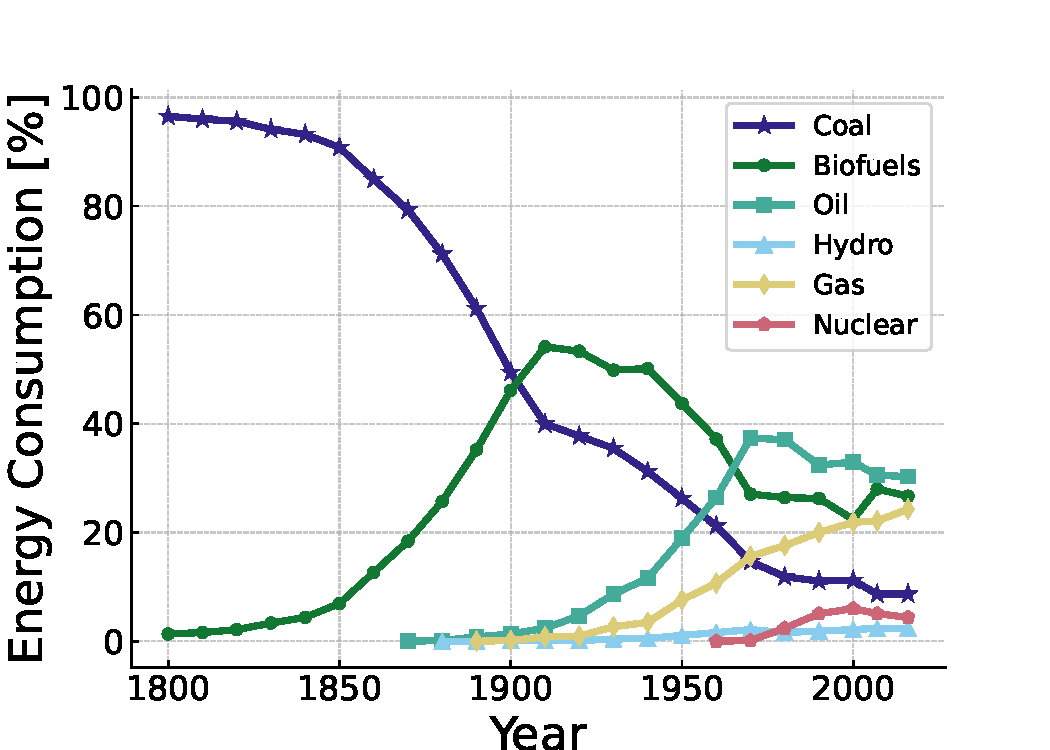
\includegraphics[width=0.499\textwidth]{images/leg_frame/proportional_fuel_use.pdf}
 }
  \hfill
  \subfloat[Total Energy Use.\label{fig:total}]{%
    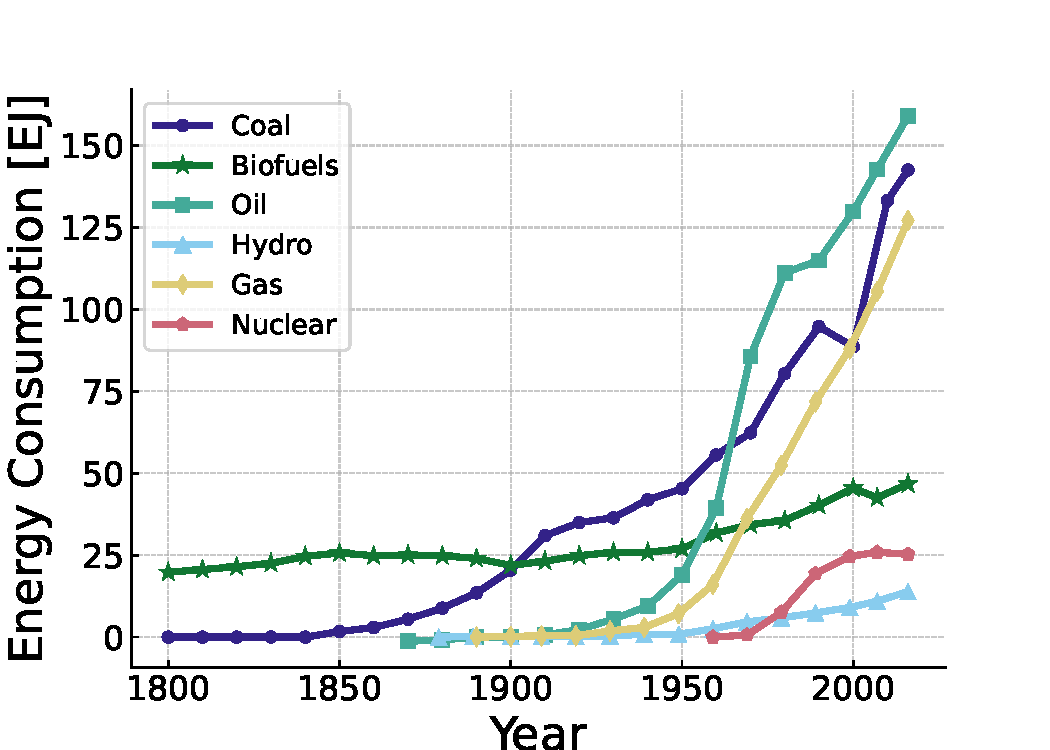
\includegraphics[width=0.499\textwidth]{images/leg_frame/total_fuel_use.pdf}
 }
  \caption{
    Global energy consumption (exajoules) by source. 1800--2017
    \cite{york_energy_2019}.}
  \label{fig:percent_total_energy}
\end{figure}

Similarly, what looks in Figure \ref{fig:percent} like a transition away from
coal in the early 1900s, with the introduction of alternatives like oil and
hydroelectricity, belies the continued increase in coal consumption into the
early 2000s. If what we have axiomatically understood as a transition is not
happening, we arrive at the kernel of several grand challenges to our society
and our elected officials. The semantic difference between a transition and a
displacement is not the core concern, instead we must focus on realistically
presenting the increasing energy needs of our society.

The policy inertia behind the monetary valuation of our energy system is
something that future generations could overcome, upending the incentives
policymakers might implement to drive an actual transition instead of a
displacement as we have discussed. If decision-makers focus on what a policy
will do only for the term of their service, they drastically undervalue the
impact that daily climate actions will have hundreds of years down the line. We
see this dichotomy in the 2020 grid failings in Texas during the unseasonably
cold front they experienced. From the outside, we can see how an extreme
weather event would create a great demand. This case is a microcosm of a
drastic change in the values a society had in an energy grid. In the span of a
couple of weeks a state that had proudly touted its achievement of a sustained
grid \cite{texas_ercot_nodate} experienced massive failures only for its
service to resume.

Since 2020, the \gls{ercot} has been working to update its grid to be more
resilient to such events, the Grid Deployment Office of \gls{doe} published a
report in 2024 outlining the more than \$270 billion of savings from increasing
connections to the Texas Interconnection
\cite{doe_transmission_planning_study_2024}. Concurrent with this announcement,
the \gls{doe} announced \$1.5 billion transmission investment that would go to
four projects in Texas, New Mexico, Louisiana, Mississippi, Maine, Oklahoma,
and Arizona \cite{doe_tran_announce_2024}. These projects are expected to be
completed by 2026 and will increase the capacity of the grid by 1.5 GW. This is
a step in the right direction, but it is not enough to ensure that the grid
will be resilient to future extreme weather events.

We can legislate for such changes by developing policy frameworks that bring in
the community and address our changing values for energy systems. Elisa Papadis and George Tsatsaronis set out to update the vision for a well-designed policy package in their 2020 paper, surmising that producing policy "with measures such as carefully introduced targeted investment subsidies, performance standards and mandates, communication and education campaigns and a CO$_2$ tax for global aviation and shipping" constitutes achieving this legislative framework \cite{papadis_challenges_2020}. This approach will require geographically bespoke solutions that draw in stakeholders, and focus on serving the needs of the future stakeholders as well as the current ones. They go on to advocate for expansion and investment in the massively complex \gls{usa} power grid due to the requirements of more flexibly generated capacity.

Flexibility is a seemingly ubiquitous goal of decarbonized industries, like
chemical producers, which highlight big emitters that are large volume/
low-profit goods (disincentivizing development)
\cite{mallapragada_decarbonization_2023} or farm researchers who highlight the
growing importance of human intervention as climate change impacts their crop
in a negative feedback cycle \cite{farokhi_soofi_farm_2022}. The start is
focusing our efforts where investment can have the largest impact in the
shortest time, and to consult the changing valuation of stakeholders in how we
deploy electrification and updates to the grid.

\section{Energy System Modeling}
\label{sec:esm}

Countries like the \gls{usa} and \gls{uk} often centralized their electrical
infrastructure as it developed, which resulted from an attitude that Dieter
Helm from the University of Oxford describes as being prevailing until the end
of the 1970s \cite{helm_energy_2002}. Due to the heavy state involvement,
energy planning is a concept that has existed for many decades. Evidence of
this contemporary category of planning can be found as far back as 1967 in
nationalized industry reports from the \gls{uk}
\cite{treasury_nationalised_1967}, and was a top-of-mind consideration in the
\gls{usa} and other countries as well.

In 1973 Michael Posner from the University of Cambridge published his book
\textit{Fuel Policy A Study In Applied Economics} \cite{posner_fuel_1973},
which set out to describe methods that large institutions could use to make
energy decisions. This book, in connection with the 1973 oil crisis, served as
a wake-up call for many countries to enhance their predictive capabilities for
energy markets. The crisis led to the development of energy planning models
that could be used to evaluate the impact of different policies on energy
systems as disruptions tend to do \cite{plazas_disrupt_2022}. The \gls{iiasa},
founded in 1972, and the \gls{iea}, founded in 1974, are two organizations that
have since served international communities with \gls{esm} tools since the oil
crisis. The resulting models were used to develop long-term energy plans to
help countries increase their energy security, facilitate economic development,
and better legislate with increasingly complex energy systems.

Today, utilities, countries, and other organizations use \glspl{esm} to model
the behavior of energy systems in different economic contexts, such as the cost
of energy, the price of carbon, and the availability of financing. These
contexts can focus on developing favorable conditions for new technologies,
understanding the relationship between actors, predicting future trends, and
the impact of different policies on energy systems. Decision-makers compare the
behavior of energy systems in various scenarios to a baseline, such as
business-as-usual scenarios compared with low-carbon or high-renewable
scenarios. These are effective across regulated, competitive, and hybrid
markets. As \glspl{esm} have evolved, they have become more sophisticated. Now
they can model the behavior of energy systems in different social contexts,
such as the adoption of energy efficiency measures, the acceptance of energy
technologies, and the resistance to new energy projects. The Osier tool
\cite{Dotson_osier}, for example, is a
framework for multi-objective optimization over traditional cost constraints
that incorporates public preferences and user-defined parameters.

Pfenninger et al. \cite{pfenninger_energy_2014} describe four
paradigms of energy system modeling: optimization, simulation, econometric, and
hybrid models. In the optimization paradigm, the modeler seeks a normative
solution to a problem by minimizing or maximizing an objective function subject
to constraints. In the simulation paradigm, the modeler aims to predict the
behavior of the energy system by simulating the interactions between different
system components. In the econometric, or market, paradigm, the modeler seeks
to understand the relationship between different operational variables in the
energy system by estimating the parameters of a statistical model. The hybrid
paradigm is a catch-all for narrative scenarios that combine the paradigms to
develop a more comprehensive understanding of the energy system.

Although there are myriad paradigms of \gls{esm}, two philosophies (top-down
and bottom-up) to their construction dictate the restrictions your model will
place on the type of questions you can answer. In the top-down approach, the
modeler starts with a high-level view of the energy system and then drills into
the details. This approach aids in understanding the overall behavior of the
energy system and the impact of different policies on the system
\cite{laha_energy_2017}. In the bottom-up approach, the modeler starts with the
details of the energy system and then builds up to a high-level view. This
approach is useful for understanding the behavior of individual components of
the energy system and the impact of different technologies on the system
\cite{ipcc_ch2_2000,laha_energy_2017}.



In the US, we keep each of these facilities separate in the front-end of
the fuel cycle in a "collect and wait" pathway \cite{cycle_risks}. In
lieu of a long or interim solution for the \gls{uf}, the back end of the
\gls{nfc} is collocated with the reactors that burn the fuel (with the
minor exception of the consolidated storage facility in Morris Illinois).

Nuclear fuel has the capacity to be
reprocessed and recycled into a different fuel type that can produce
usable power for several cycles, called a "closed" fuel cycle.





 \begin{figure}[h]
    \centering
    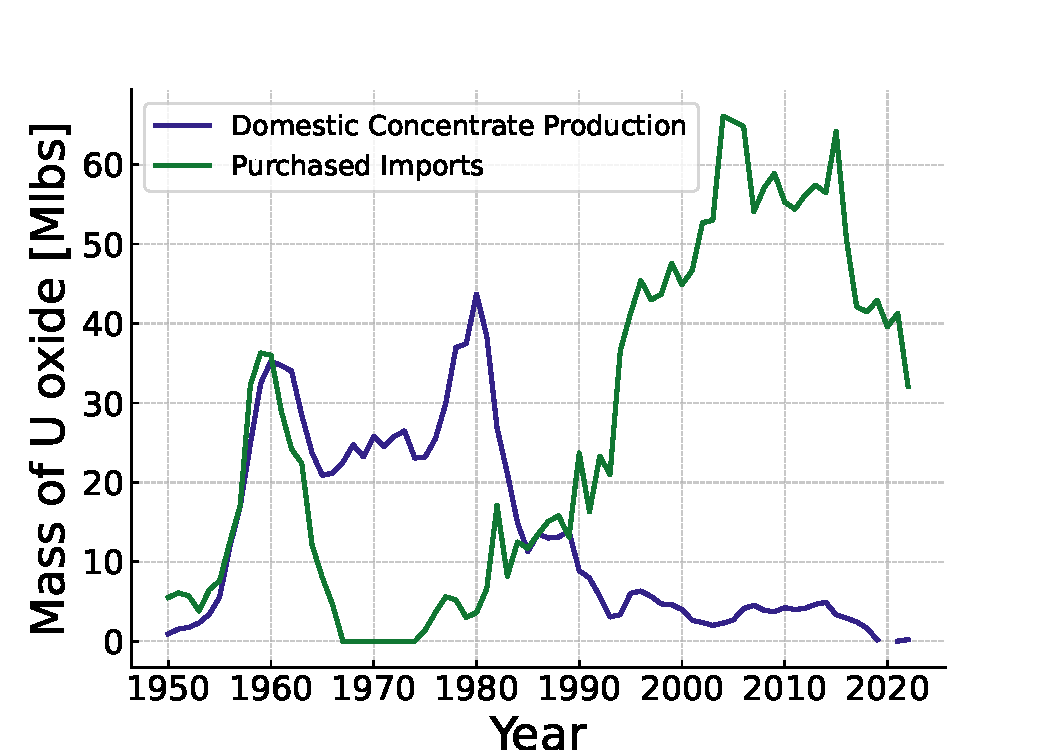
\includegraphics[scale=0.8]{images/intro/uranium_production_imports.pdf}
    \caption{Foregin and domestic uranium purchases over time \cite{eia_monthly_energy_review_2024}.}
    \label{fig:foregin_u3o8}
 \end{figure}

\section{\cyclus}
\label{sec:cyclus}
% fix that, too informal and introduces archetypes without context.
\cyclus is an agent-based \gls{nfc} simulator that is versatile, open source, and modular. The software achieves this versatility through a series of generic archetypes that are primarily transaction based. Over the years, the user community and developers have created a litany of nuclear specific archetypes for everything from proliferation assessment to fuel burnup. Many standard fuel cycle facilities have been implemented in the \cycamore repository on GitHub, which holds technology-agnostic archetypes for material sources, material sinks, enrichment services, separations capabilities, and a generic reactor.

% discuss recipes
As \cyclus is a transactions code and not necessarily a physics code,
the reactors incorporate reactor physics through pre-defined "recipes,"
where the user specifies the isotopic concentration of the fresh and
used fuel.

Users approximate the burnup of each fuel element with the
same input recipe as the same; however, in this work we incorporate a
cascading enrichment from \gls{leu+} to \gls{haleu}.
% find a citation or source that companies are actually going to do that
% (best case scenario is find it for each reactor you do it for)

% discuss EVER and CLOVER?
Novel in this work is our use of a low fidelity archetype based on the
\cycamore reactor %\cite{the summer poster}. \gls{ever}

\gls{ever} allows the user to specify multiple recipes for the fuel and
change between them at specific times.


% discuss DRE
As we have discussed, \cyclus's primary function is to keep track of
material transactions between agents. This is accomplished through the
\gls{dre}, which functions like a market where each agent brings a bid
for what and how much material they need and suppliers are matched with
buyers % cite something here.


\subsection{Archetypes and Time Management}
\label{sec:archetypes_and_time_management}

Throughout the \cyclus ecosystem, archetypes interact with the \gls{dre} and each other in a fixed, user defined, time step, forcing the entire simulation to operate on the smallest universal time step. For example, if a fabrication facility can produce material every 2 months but the enrichment facility can only provide material every 3 months, then we would need to use a 1 month time step to capture both. When the time step is smaller than the minimum for a given facility, that facility still participates in the \gls{dre} with a 0 bid. These zero bids, across hundreds of facilities, add complexity and inefficiencies to solving the transaction problem at each time step.

Examining the \cyclus ecosystem, we identified an archetype called $Pattern_Sink$ wherein the user can alter the frequency that the material sink, often called the repository, can accept material. We have created an example of this archetype in action with a simple A-B-C scenario, shown in Figure \ref{fig:a-b-c}. In this scenario, material is received from a source (A) to a reactor (B) with a final (C) sink that can only accept material at a certain frequency.

\begin{figure}
    \centering
    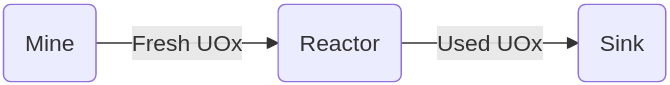
\includegraphics[scale=0.4]{images/cyclus/a-b-c.png}
    \caption{Simple A-B-C Scenario}
    \label{fig:a-b-c}
\end{figure}

If we track the material being received by the sink it becomes clear that this frequency simply alters how frequently the archetype updates its internal understanding of time. As a consequence, it appears in Figure \ref{fig:pattern_freq_50} as though multiple groups of material are received in one time step despite this archetype not having an idea of individual shipments. The way this archetype accomplishes the artificial restriction on accepting material is by simply not updating the time step that the archetype is at until the next universal time step is met. Regardless of function, this is the only example of flexibility of timestep we found in the ecosystem.

\begin{figure}
    \centering
    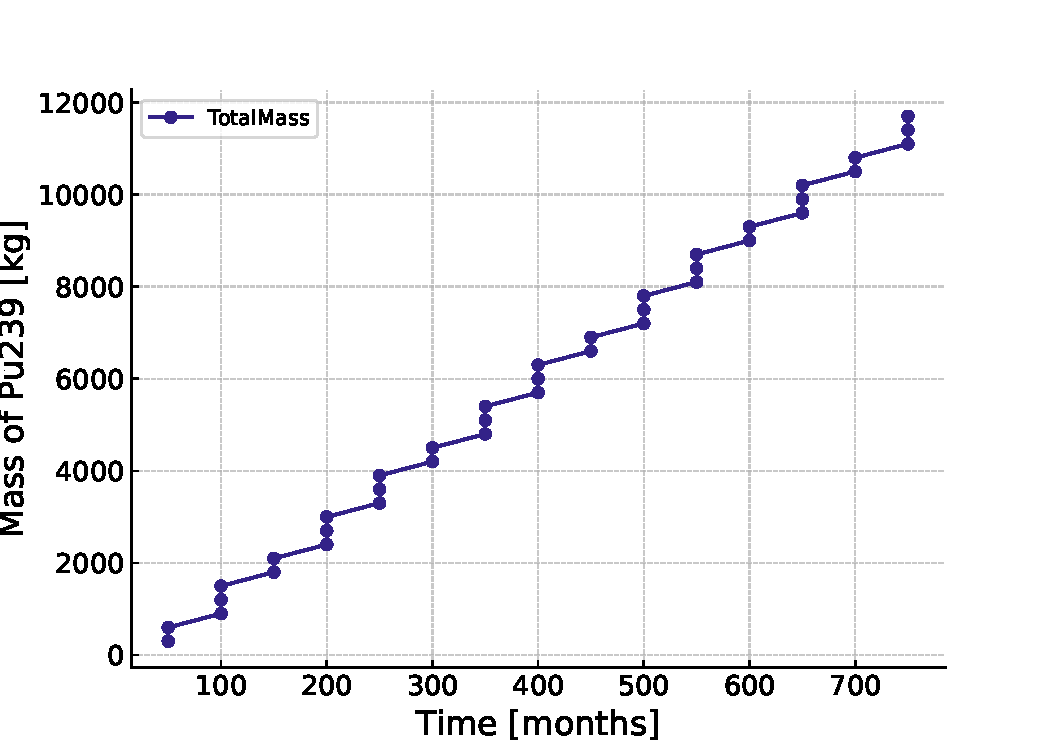
\includegraphics[scale=0.4]{images/cyclus/pattern_sink_fuel_transactions.pdf}
    \caption{Production of $^{239}$Pu with a frequency of 50 months}
    \label{fig:pattern_freq_50}
\end{figure}

In this work we implement a fundamental toolkit capability that any archetype in the Cyclus ecosystem can take advantage of with one implementation.


\section{Fuel Enrichment}
\label{sec:leup}

In 2020, a \gls{haleu} workshop report led by Monica Regalbuto \cite{regalbuto_high_assay_2020} highlighted the unique regulatory challenges of establishing a \gls{haleu} fuel cycle in the \gls{usa}. It noted that part of enriching \gls{haleu} is first to produce \gls{leup}, defined as between 5\% and 10\% $^{235}U$ enrichment. The report notes that \gls{leup} facilities would fall under a similar category of regulations as the existing \gls{leu} fuel cycle, allowing existing enrichment servicers to leverage their experience and infrastructure before taking on the increased regulatory burden of producing \gls{haleu}. If a reactor could be redesigned to accommodate it, using \gls{leup} could delay the demand for \gls{haleu}. Table \ref{tab:enrichment_levels} shows the various levels of enrichment for uranium fuel in the \gls{usa}

\begin{table}[H]
   \centering
   \caption{Enrichment levels and their ranges.}
   \label{tab:enrichment_levels}
   \begin{tabular}{l l}
      \hline
      \textbf{Enrichment Level} & \textbf{Range [\%  $^{235}$U]} \\
      \hline
      Natural & < 0.711 \\
      \gls{leu} & 0.711-5 \\
      \gls{leup} & 5-10 \\
      \gls{haleu} & 10-20 \\
      \gls{heu} & $\geq$ 20  \\
      \hline
   \end{tabular}
\end{table}

One of the primary advantages of a fuel cycle containing \gls{leup} is that the facility to produce it would fall under the same licensing category as \gls{leu} fuel. The \gls{nrc} defines a \textit{special nuclear material of low strategic significance} as meeting one of three criteria, the most notable of which for the purposes of this thesis is "(3) 10,000 grams or more of uranium-235 (contained in uranium enriched above natural but less than 10 percent in the U–235 isotope)," \cite{nrc_catiii}. This facility definition is where the upper limit of the \gls{leup} range arises.

Facilities like Centrus in Piketon, Ohio enrich \gls{haleu} fuels compliant with regulations for \textit{special nuclear material of moderate strategic significance} (Category II), but the commercial facilities in the \gls{usa} do not have contemporary experience enriching \gls{haleu} fuels and this demonstration will need to be expanded to support a fleet of higher enriched reactors. Additionally, Category II facilities come with increased construction and operation costs that would increase the barriers to establishing these facilities before a consistent demand has been established. Thus, \gls{leup} is an attractive intermediary step for servicers wishing to minimize the size of a Category II facility (thereby reducing costs) as it is the same category as historically licensed enrichment facilities for \gls{leu}.

Traditional \glspl{lwr} could receive benefits from using \gls{leup} fuel; as outlined by L\'{o}pez-Luna et al. \cite{24_month_cycle_bwr}, incorporating such fuel rods would allow for a 24-month cycle in the \gls{bwr} design they studied and would reduce the levelized cost of the nuclear fuel cycle they simulated. In October 2024, Framatome announced that their 6 wt$\%$ $^{235}$U GAIA fuel assemblies completed their third 18-month fuel cycle at the Vogtle plant in Georgia \cite{framatome_press_2024}, with the eventual goal of this process being commercialization of new accident-tolerant fuels that can potentially support \gls{leup}.

Increased prevalence of higher enrichment fuels will require modifications to the existing supply chain, particularly to ensure the continued safety of workers and the public. A 2022 report from Shaw and Clarity out of \gls{ornl} highlighted that existing nuclear fuel vault configurations at \glspl{bwr} and \glspl{pwr} did not have sufficient margins to satisfy regulatory requirements when fully flooded \cite{leup_atf_storage_impacts}. Their report only studied the impacts of 6.5 wt$\%$ and 8 wt$\%$ fuel, but they concluded that \gls{haleu} fuel would similarly require significant changes to existing fuel storage infrastructure.

\section{TRISO Fuel}
\label{sec:triso_fuel}

In this work, we adapt the approach of Bachmann et al.
\cite{bachmann_enrichment_2021} to focus on \gls{triso} fueled reactor designs
alongside traditional fuel forms at various enrichments. \gls{triso} is not a
classification of enrichment; several reactor designs use different fuel
enrichments that are all \gls{triso}. Here we will distinguish the
production of \gls{triso} from the traditional metallic fuels used in
\glspl{lwr} outlined in Section \ref{sec:nfc}.

Coating the fuel particles is a critical step in the fabrication of \gls{triso}
fuel, and the idea has existed in nuclear fuel design spaces since the 1950s
\cite{price_dragon_2012} with the Dragon project. In 1957, the Harwell facility
began coating spherical fuel particles, and in 1961, researchers modified the
particle coating to include a silicon carbide layer to trap cesium, strontium,
and barium--which diffused through the single pyrolytic carbon layer.
Concurrently, in 1958, a report to the \gls{aec} introduced the concept of a
pebble bed pile (first proposed by Daniels
\cite{f_b_daniels_suggestions_1944}) to the broader nuclear community.
Researchers in Germany, China, and the UK have proposed, built, and operated
similar designs since then, with companies in the \gls{usa} looking to deploy
modern versions of the technology.

In a 2019 paper, authors Demkowicz, Liu, and Hunn \cite{particle_review_2019}
authors describe the fuel as a particle encapsulated in layers of pyrolytic
carbon and silicon carbide; a \gls{fbcvd} applies each of these layers. As
shown in Figure \ref{fig:triso_layers}, the layers are frequently ordered with
a fuel kernel at the center, followed by layers of porous carbon buffer, inner
pyrolytic carbon, silicon carbide, and outer pyrolytic carbon. The fuel kernel
is typically composed of uranium dioxide, and it is surrounded by a porous
carbon buffer using acetylene in the \gls{fbcvd} as it has a relatively low
density. The silicon carbide layer encapsulates the pyrolytic carbon layers and
provides a barrier to fission products. A mix of methyltrichlorosilane and
hydrogen is sufficient for SiC deposition without argon. The inner and outer
pyrolytic carbon layers isolate the silicon carbide layer and provide a barrier
to the coolant; the \gls{fbcvd} applies these layers using a mix of propylene,
acetylene, and argon.

\begin{figure}[H]
    \centering
    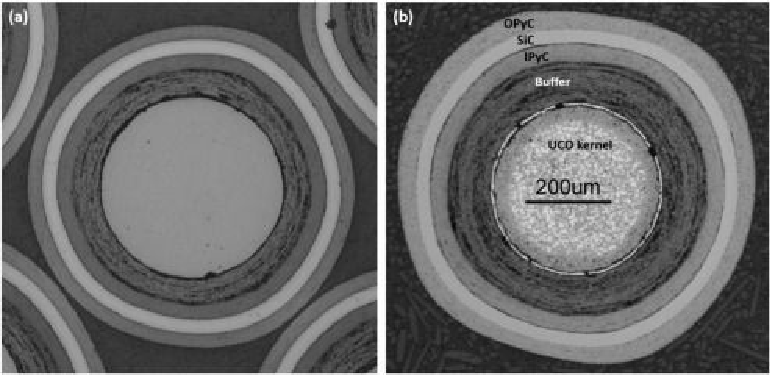
\includegraphics[scale=0.98]{images/triso_review/triso_layers.pdf}
    \caption{TRISO Fuel Particle Layers \cite{particle_review_2019}}
    \label{fig:triso_layers}
\end{figure}

Through a heat and pressure setting process, fabricators create a fuel matrix
that accepts the coated particles. These matrices hold the \gls{triso}
particles in graphite and carbonized resin and are set under heat and pressure,
often overcoated to prevent particle-particle interactions. The resulting fuel
type is incredibly robust and can reduce proliferation concerns due to the
difficulty separating the particles from the matrix and the fuel from the
particles. The fuel can withstand high temperatures and burnups, which can be
advantageous in reactor designs that require high temperatures for efficient
operation.

\section{Reactor Models}
\label{sec:reactor_models}

This thesis explores various transition scenarios for the deployment in the \gls{usa} of the: 1) \gls{xe} \gls{htgr}; 2) \gls{usnc} \gls{mmr} \gls{htgr}; and 3) and Westinghouse AP1000 \gls{pwr}. To accommodate the assumption that the \gls{haleu}-fueled \gls{triso} reactors will first accept \gls{leup} fuel, this thesis adapts Bachmann's \gls{mmr}-like Serpent model \cite{bachmann_mmr_like_2023} and Richter's \gls{xe}-like Serpent model \cite{richter_xe100_like} to accept \gls{leup} fuel. These reactor models are constructed from publicly available data to approximate their aggregate behavior.

Table \ref{tab:ar_defs} shows the design specifications for the advanced reactors in this thesis. The \gls{mmr} and \gls{xe} reactors are \gls{htgr}s that use \gls{triso} fuel, while the AP1000 is a \gls{pwr} that uses UO$_2$ fuel. The enrichment distinguishes the versions of the \gls{mmr} and \gls{xe} as the only distinguishing variable between the two versions of the reactors. The cycle length, discharge burnup, and reactor lifetime are the same for both versions of the reactors. The AP1000 is assumed to use \gls{leu} fuel throughout the simulation. The \gls{mmr} is the smallest power output reactor in this thesis, and can serve as a representative of mix of small, \gls{triso}-fueled reactors. The \gls{xe} reactor is an order of magnitude larger in power output, and can be considered a representative of larger, \gls{triso}-fueled reactors. The AP1000 is the largest reactor in this thesis and is a representative of gigawatt-scale reactors.


\begin{table}[H]
   \centering
   \caption{Advanced reactor design specifications.}
   \label{tab:ar_defs}
   \begin{tabular}{l l l l}
      \hline
      \textbf{Design Criterion} & \textbf{MMR-Like} \cite{usnc_design_2021} & \textbf{\gls{xe}-Like} \cite{nuscale_chapter_2018} & \textbf{AP1000} \\
      \hline
      Reactor type & \gls{htgr} & \gls{htgr} & \gls{pwr} \\
      Power Output [MWe] & 15 & 100 & 1000 \\
      Fuel Type & \gls{triso} & \gls{triso} & UO$_2$ \\
      Enrichment [\% $^{235}$U] & 9.95, 19.75 & 9.95, 15.5 & 5 \\
      Cycle Length & 20 [yrs] & Online Refuel & 18 [months] \\
      Discharge Burnup [GWd/MTU] & 82 & 168 & 65 \\
      Reactor Lifetime [yrs] & 20 & 60 & 60 \\
      \hline
   \end{tabular}
\end{table}

The following subsections discuss the reactors in greater detail. These models  approximate that the \gls{leup}-fueled reactors achieve the same burnup, power level, and core lifetime as the \gls{haleu}-fueled version. These assumptions are sufficient for the metrics outlined in Section \ref{sec:metrics} as this thesis does not perform \gls{uf} isotopic analysis, but could stretch the \gls{uf} temporal profile.



\subsection{MMR-like Reactor}
\label{sec:mmr}

In 2021, \gls{uiuc} submitted a notice of intent to the \gls{nrc} detailing their plans to apply for a construction permit of the \gls{mmr} reactor from \gls{usnc} \cite{uiuc_notice_nrc_2021}. Activities have continued as \gls{uiuc} continues the project, they reached the pre-licensing phase with the \gls{nrc} and were planning on commencing operation of an on-campus reactor in the 2030s. This \gls{mmr} is an \gls{htgr} that uses \gls{triso} fuel, has an electrical output of 15 MW$_e$, and a cycle length of 20 years. The fuel is enriched to 9.95\% $^{235}$U for \gls{leup} and 19.75\% for \gls{haleu}. As modeled, both have a discharge burnup of 82 GWd/MTU, which coincides with the 20-year lifetime of the reactor. In this thesis, the \gls{mmr} is based on the model developed by Bachmann et al. \cite{bachmann_mmr_like_2023} and is implemented here as-is for the \gls{haleu} version of the reactor, while the \gls{leup} version updates the fuel composition from the \gls{haleu} version.

Figure \ref{fig:mmr_design} shows a rendering of the \gls{mmr} core and reactor vessel. As indicated by the figure, the design is intended to be underground, with an estimated total reactor footprint less than 5 acres. The primary coolant is helium gas, which heats up in the core and deposits its heat in a heat exchanger to generate electricity to the side of the reactor \cite{usnc_chalk_river}. Helium is transparent to many nuclear interactions and is inert, making it an attractive choice for a coolant.

\begin{figure}[H]
    \centering
    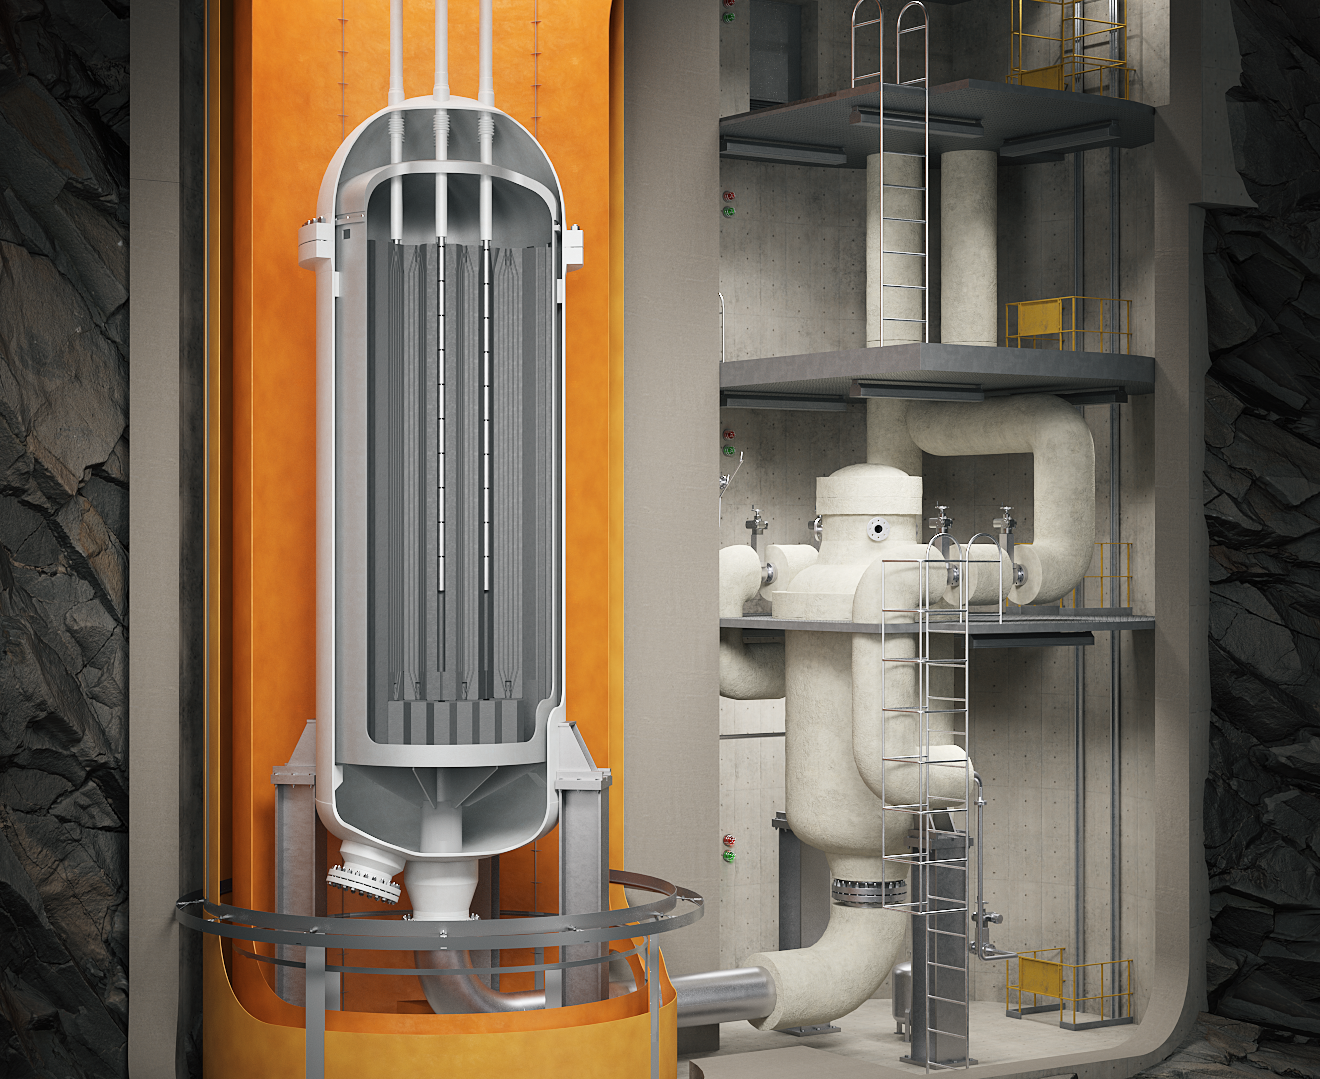
\includegraphics[scale=0.19]{images/reactor_design/wide-02.png}
    \caption{USNC MMR design \cite{usnc_design_2021}.}
    \label{fig:mmr_design}
\end{figure}

The proposed deployment of this reactor concept includes an operational \textit{\gls{mmr} Energy System} consisting of two plants: the \textit{Nuclear Plant} and the \textit{Adjacent Plant}. The \textit{Nuclear Plant} contains multiple \gls{mmr} units, including all the equipment required to transport the heat to the \textit{Adjacent Plant}. The \textit{Adjacent Plant} consists of the equipment that converts heat to electricity or process heat as needed. The \textit{\gls{mmr} Energy System} will theoretically store up to 10 hours of power plant thermal output and can be supplemented with hydrogen burners. Auxiliary molten salt thermal storage allows for a flexible electricity and process heat supply.

Electricity and heat would be delivered on demand from the power plant while the \gls{mmr} unit operates at constant power. The \gls{mmr}'s high-temperature heat has many uses beyond the generation of electricity. District heating, desalination, and chemical or industrial heat highlight the broader point of how \gls{geniv} nuclear reactors are not solely intended for electricity generation as with the current domestic fleet. An \gls{mmr} could deliver steam temperatures of 660 °C, and they estimate that temperatures up to 950 °C could be possible in future \gls{mmr} variants \cite{usnc_design_2021}.

The fuel for this reactor is inspired by the \gls{triso} fuel developed in the 1960s and 1970s. A small sphere of uranium fuel is coated in carbon and silicon carbide layers. As shown in Figure \ref{fig:usnc_fuel}, the fuel is composed of kernels arranged into a larger fuel pellet. They call their fuel form \gls{fcm} fuel. They additively manufacture each element, allowing for a high packing fraction of fuel, which means their fuel could be adapted to other reactor designs.

\begin{figure}[H]
    \subfloat[Fuel element layers.\label{fig:elemenet_layers}]{%
      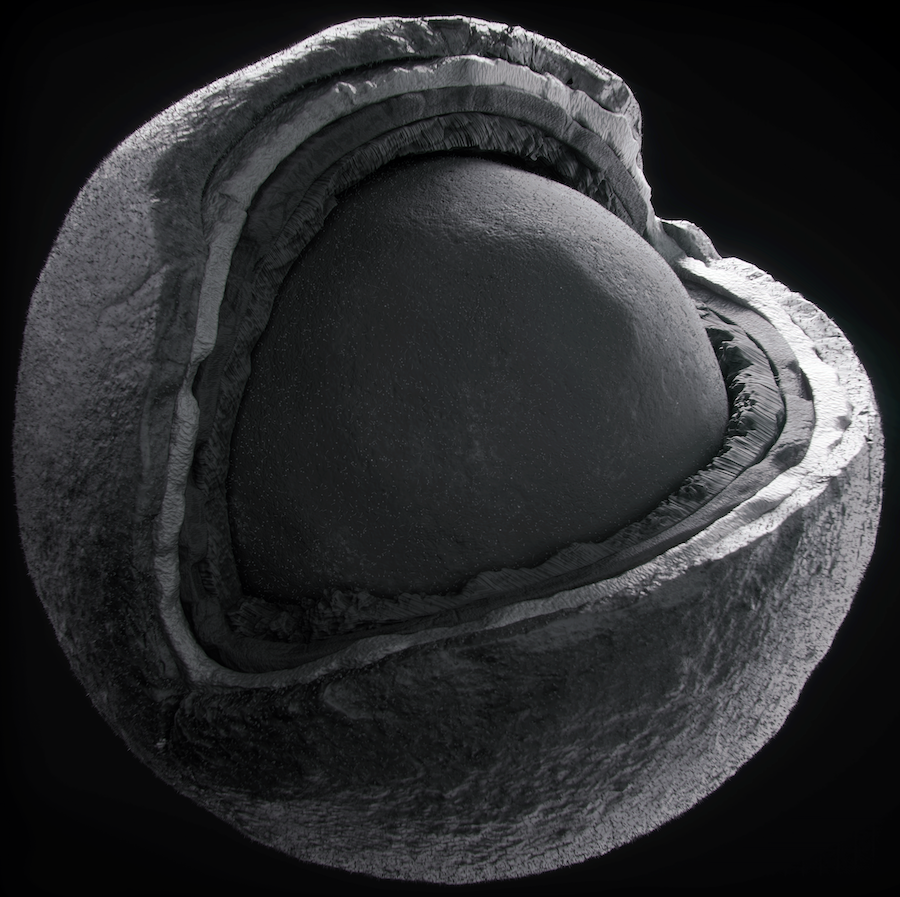
\includegraphics[width=0.49\textwidth]{images/reactor_design/usnc_triso.png}
   }
    \hfill
    \subfloat[Fuel pellet profile.\label{fig:pellet_profile}]{%
      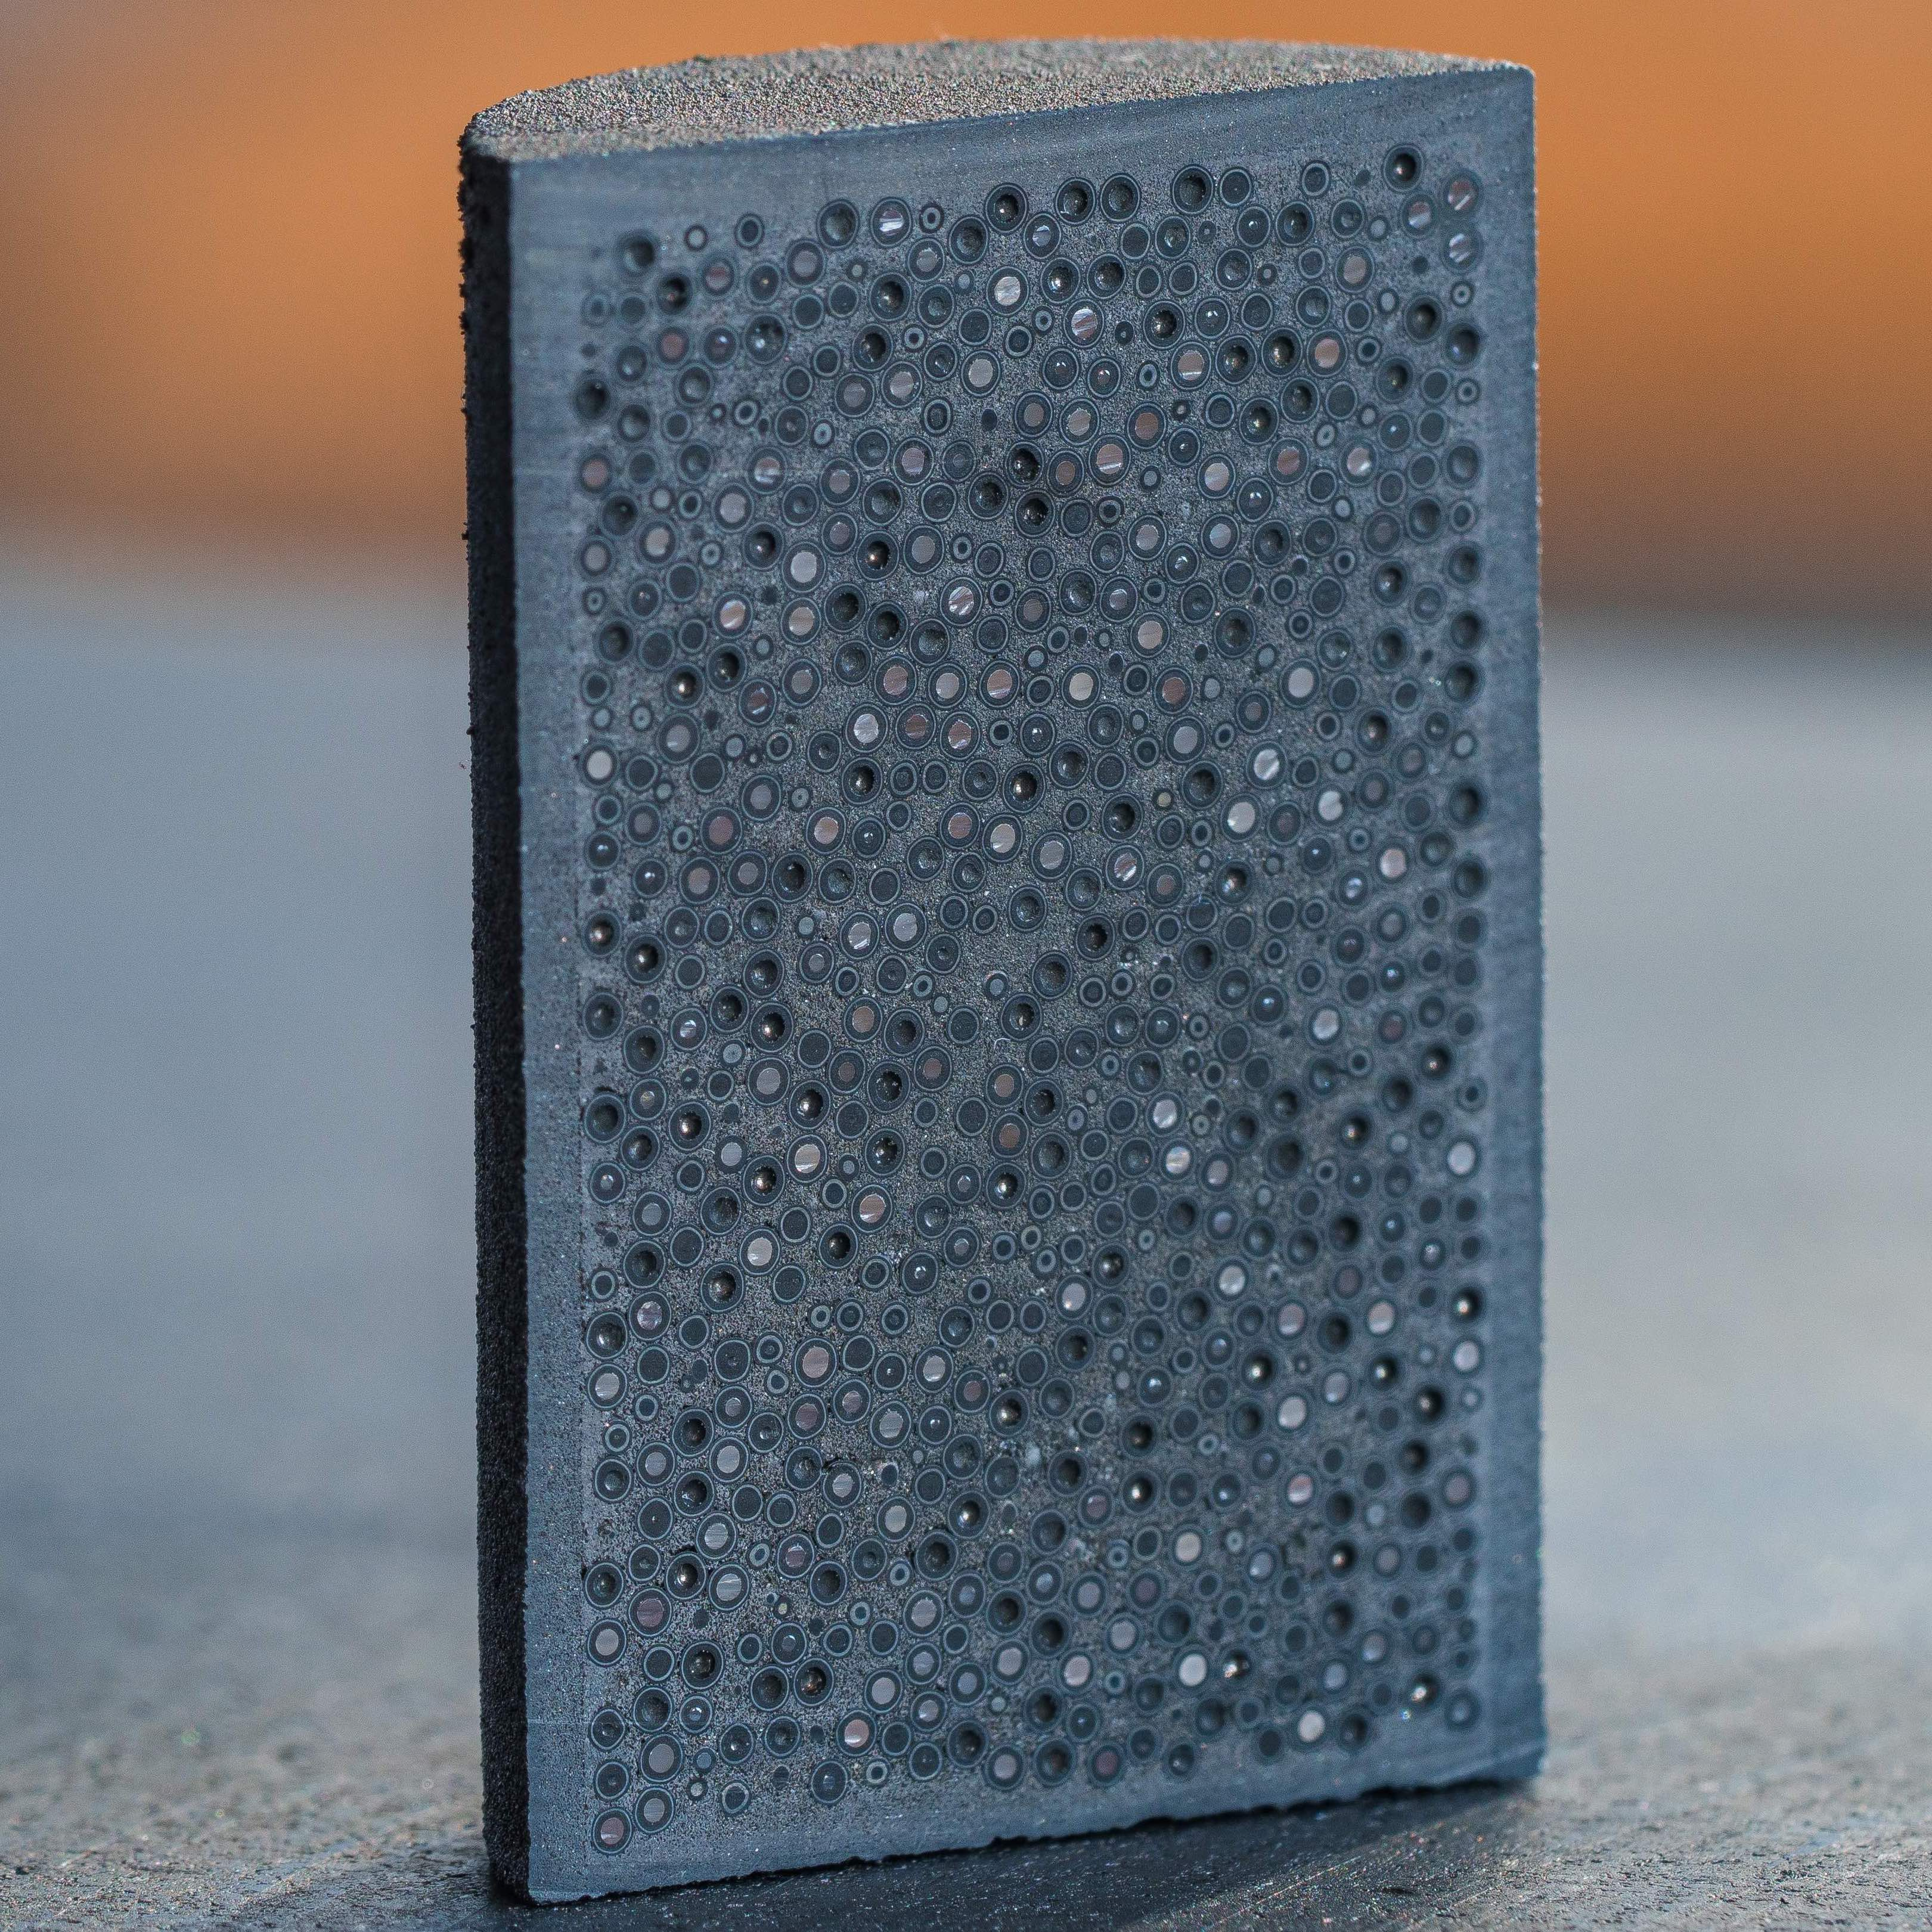
\includegraphics[width=0.49\textwidth]{images/reactor_design/usnc_fuel_side.jpeg}
   }
    \caption{
    USNC \gls{mmr} fuel renderings
      \cite{usnc_media_kit}.}
    \label{fig:usnc_fuel}
\end{figure}

Figure \ref{fig:mmr_core} shows a top-down and side view of the \gls{mmr} Serpent model \cite{bachmann_mmr_like_2023}, modified in fuel composition alone. As Bachmann describes \cite{bachmann_thesis_2023}, the radius of the fuel channel is based on the publicly available size of the \gls{fcm} pellets (1.15 cm), and the coolant channel has an arbitrarily chosen radius of 3 cm. The entire core is assumed to be in an isothermal state at 800 K. There is a 20 cm thick graphite reflector above and below the stacks of graphite and a 10 cm thick beryllium-oxide reflector on the outside of the graphite blocks of the core, illustrated by the green material in Figure \ref{fig:mmr_core}. The model does not contain control rods or burnable poisons, so the control rod tubes are filled with helium. Five layers of graphite fuel blocks are stacked to form the entire core to approximate the number of fuel blocks described in the publicly available data \cite{usnc_design_2021}. The fuel does not move through the core, as the model is designed to use the same fuel for the entire reactor lifetime.


\begin{figure}[H]
    \subfloat[Top-down core view.\label{fig:mmr_td}]{%
      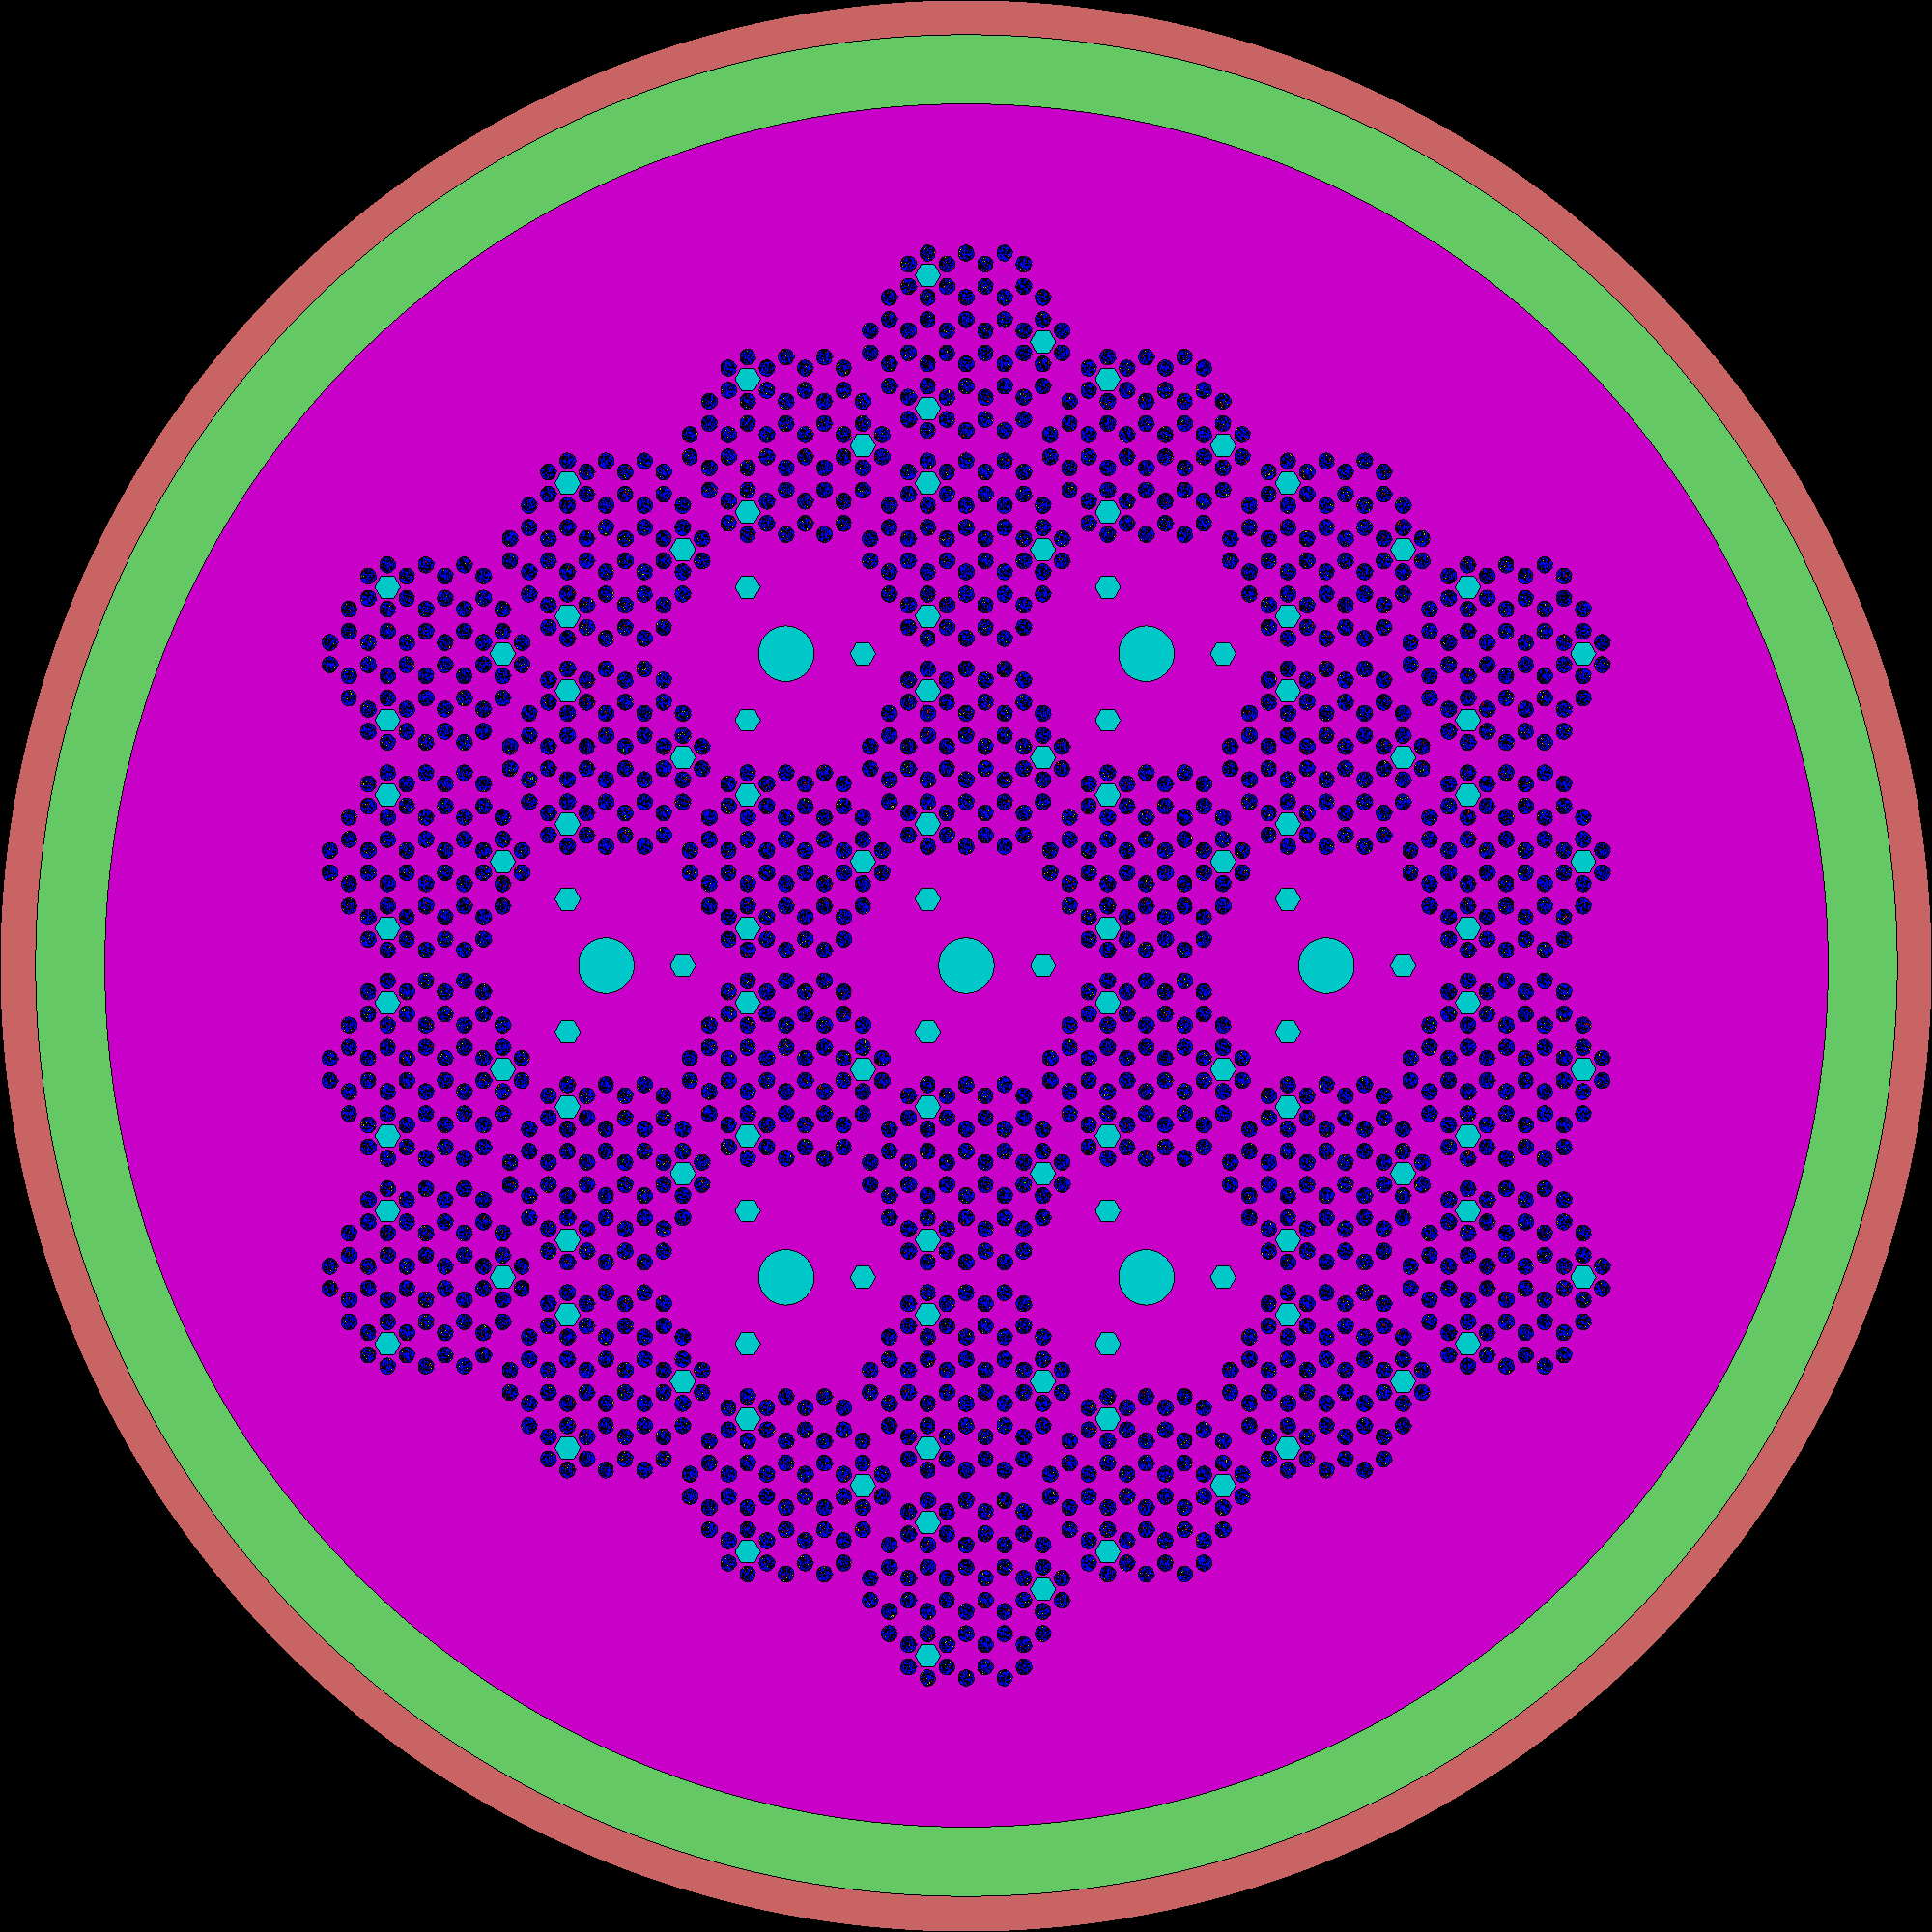
\includegraphics[width=0.49\textwidth]{images/reactor_design/haleu_mmr_2blocks.inp_geom1.png}
   }
    \hfill
    \subfloat[Full core side profile.\label{fig:mmr_slice}]{%
      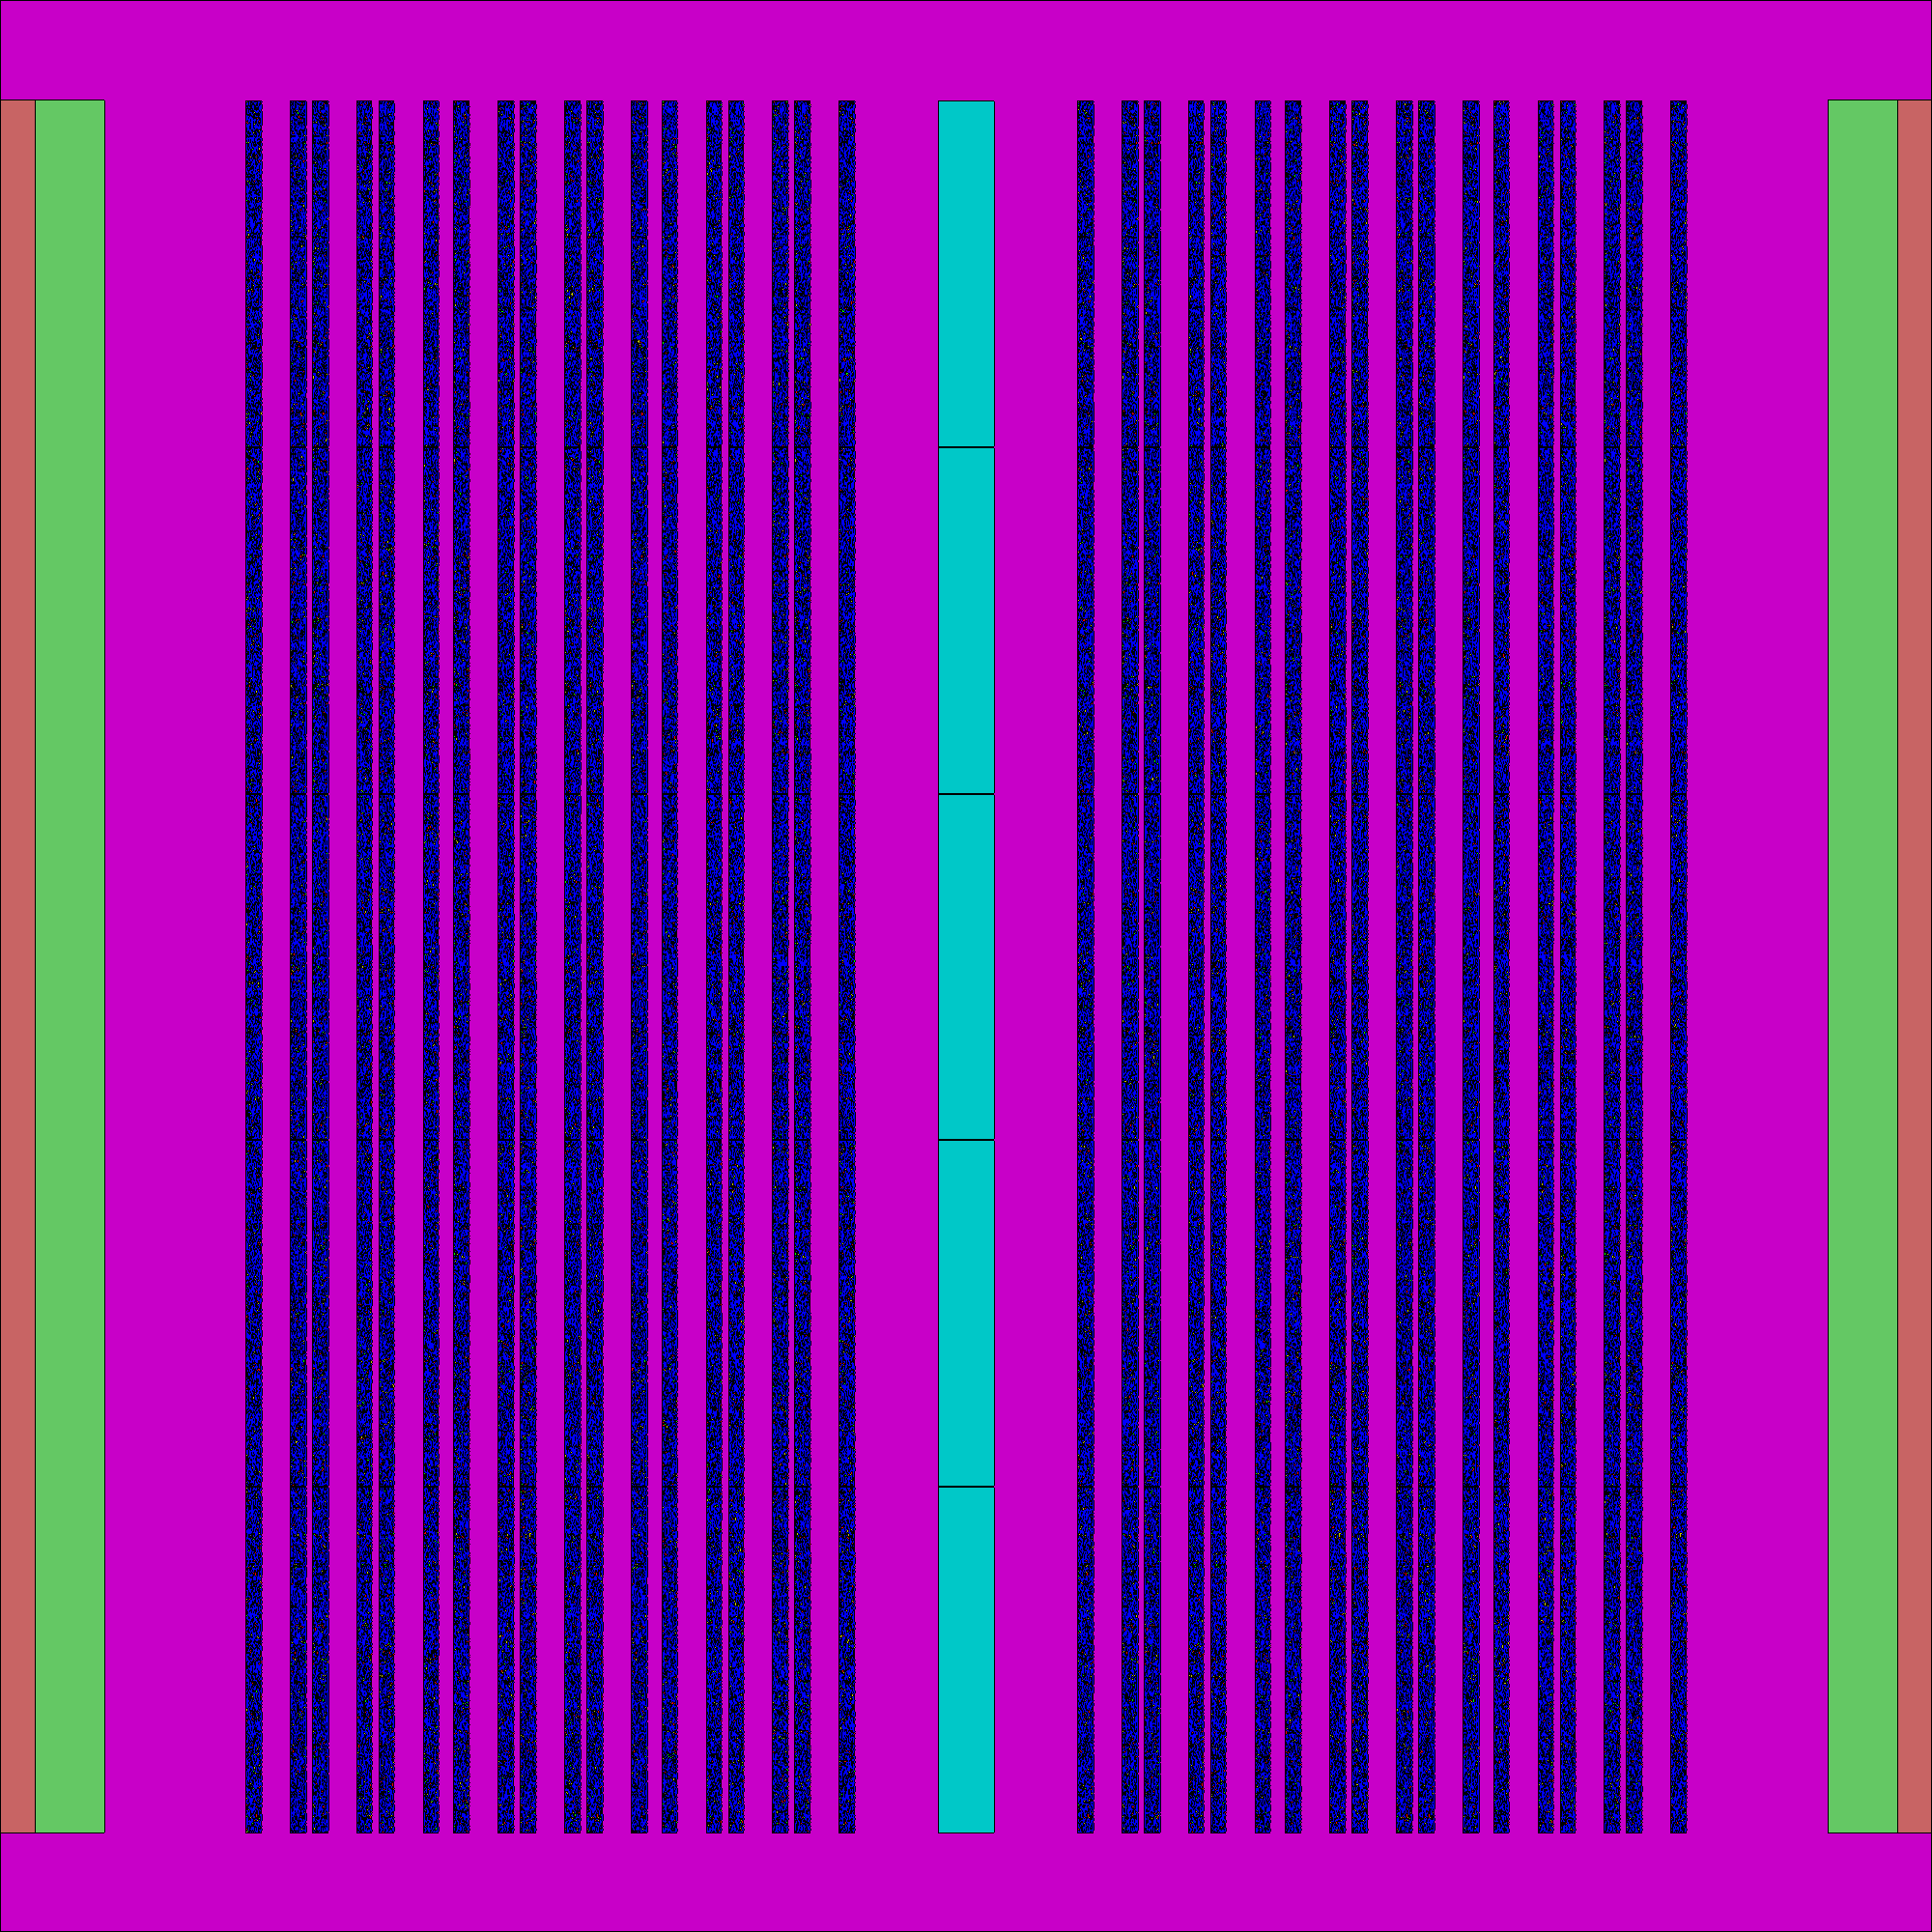
\includegraphics[width=0.49\textwidth]{images/reactor_design/haleu_mmr_2blocks.inp_geom3.png}
   }
    \caption{Serpent model of the USNC MMR core.}
    \label{fig:mmr_core}
\end{figure}



\subsection{Xe-100-like Reactor}
\label{sec:xe}

X-Energy has entered into a cooperative agreement with \gls{doe} to deploy their \gls{xe}, is in the pre-licensing phase with the \gls{nrc} for projects in Texas and Washington, and is expected to be operational in the 2030s. There are similar projects in the early stages in Canada and the \gls{uk}. The X-Energy \gls{xe} is an \gls{htgr} that uses \gls{triso} fuel and is expected to operate for 60 years. The reactor has an electical output of 100 MW and uses online refueling. The fuel is enriched to 9.95\% $^{235}$U for \gls{leup} and 15.5\% $^{235}$U for \gls{haleu} and a discharge burnup of 168 GWd/MTU. The reactor in this thesis is an approximation based on publicly available data and is not based on confidential or proprietary information. The model was developed by Richter et al. \cite{richter_xe100_like} and is implemented herein as-is for the \gls{haleu}-fueled reactor, while the \gls{leup} version has a modified fuel composition.

Figure \ref{fig:xe_design} shows a rendering of the \gls{xe} core and reactor vessel. The \gls{xe} reactor is designed to be a small modular reactor that can be deployed in various locations and will be gas-cooled. This design differs from the \gls{mmr} as the reactor features online refueling.

\begin{figure}[H]
    \centering
    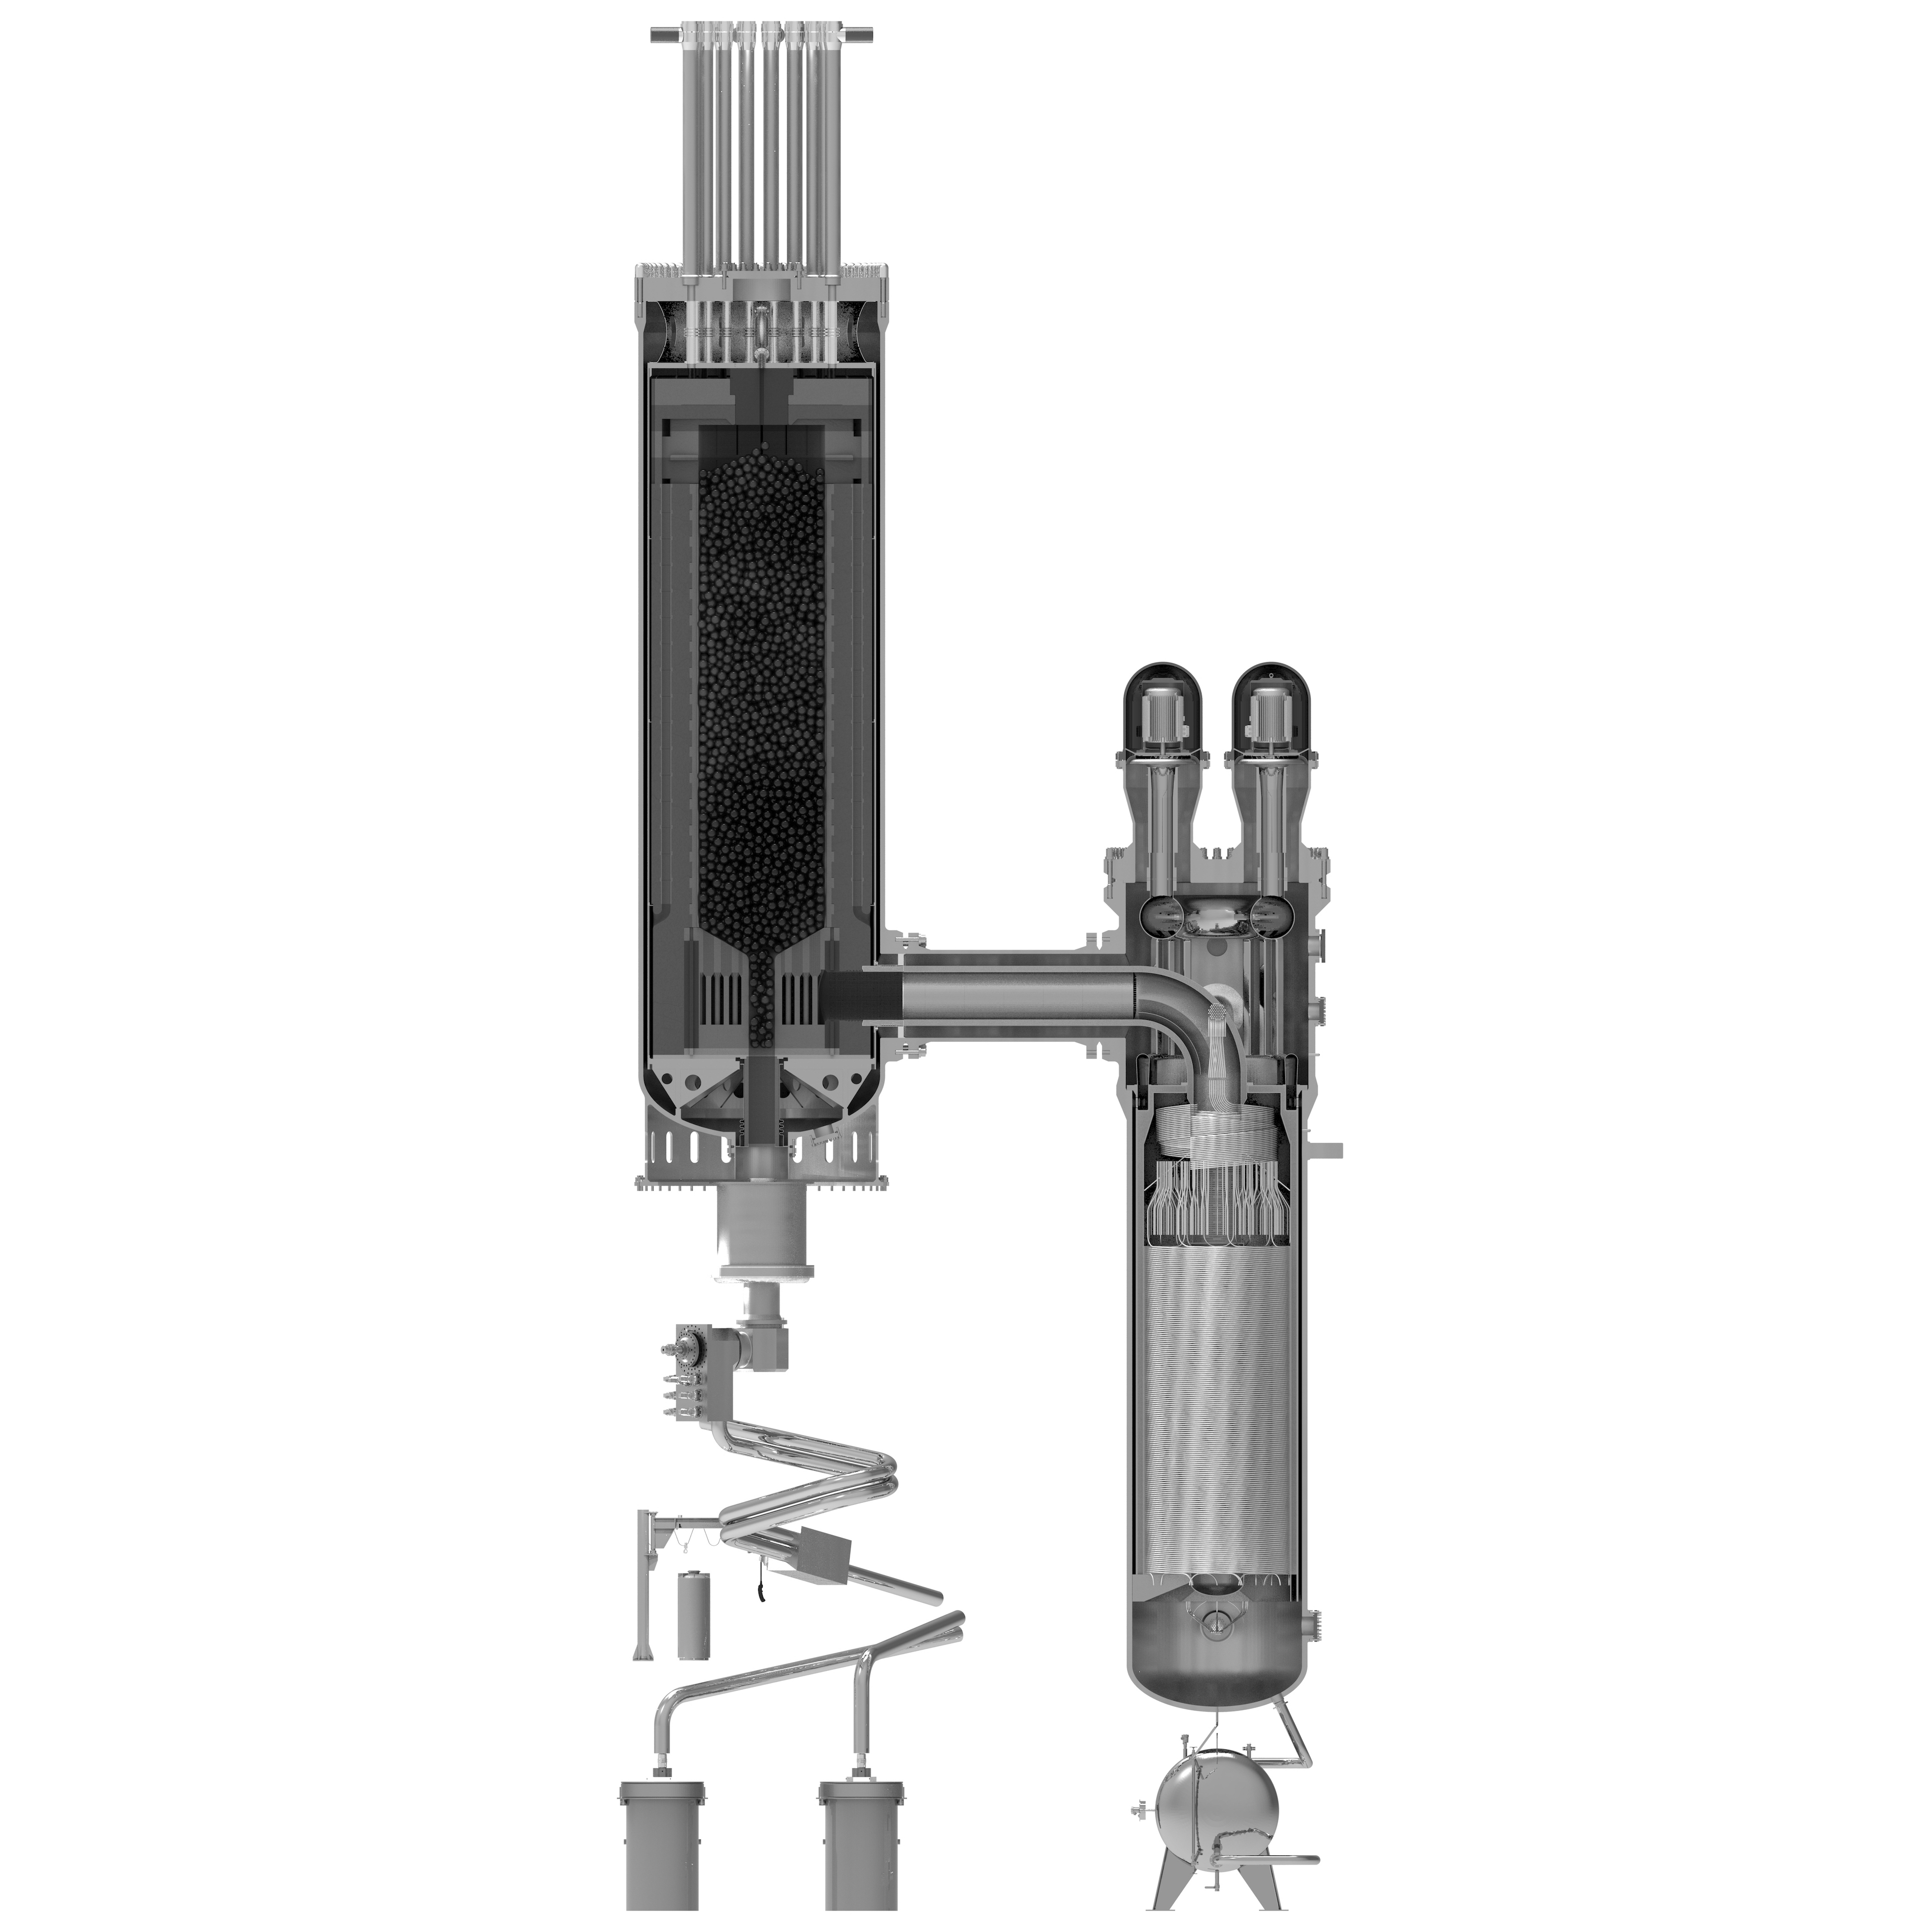
\includegraphics[scale=0.09]{images/reactor_design/xe-100-reactor-slice.jpg}
    \caption{X-Energy Xe-100 rendition \cite{xe_reactor}.}
    \label{fig:xe_design}
\end{figure}

Unlike the \gls{mmr}'s annular fuel elements, the \gls{xe} pebbles are composed of a spherical graphite matrix that contains the \gls{triso} fuel particles. These \gls{triso} particles are similar to those in the \gls{mmr}, as shown in Figure \ref{fig:xe_fuel}.

\begin{figure}[H]
    \centering
    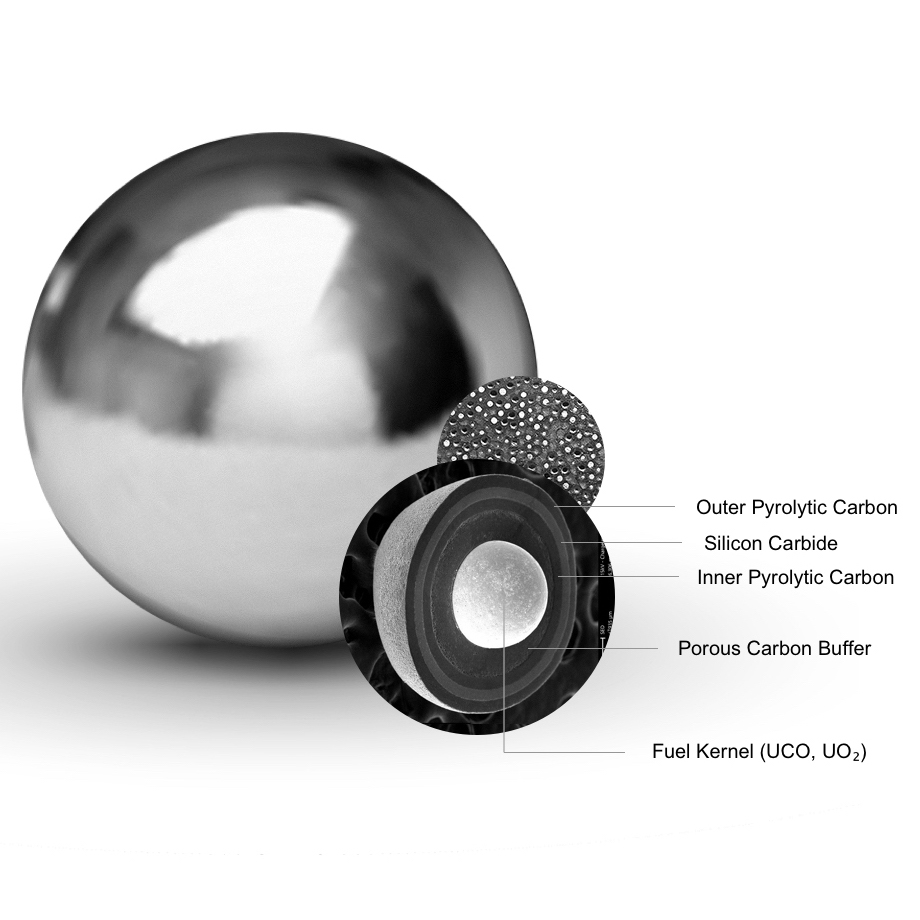
\includegraphics[scale=0.28]{images/reactor_design/graphic-triso-x-pebble.jpg}
    \caption{X-Energy Xe-100 fuel pebble \cite{xe_fuel}.}
    \label{fig:xe_fuel}
\end{figure}


This thesis modifies the fuel composition of Richter's \gls{xe}-like reactor model to accept \gls{leup} fuel. The \gls{leup} fuel is assumed to have the same burnup and power level as the \gls{haleu} fuel. This assumption, as with the \gls{mmr}-like reactor, would impact the \gls{uf} isotopic calculations. I will explore the implications in future work. Figure \ref{fig:xe_core} shows the top-down view of the \gls{leup} \gls{xe} core as the \gls{haleu} version has been established by Richter \cite{richter_thesis_2022}.

\begin{figure}[H]
    \subfloat[Initial core. \label{fig:xe_init_core}]{%
      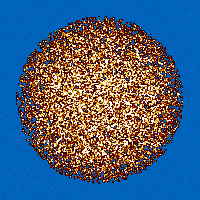
\includegraphics[width=0.49\textwidth]{images/reactor_design/htgr-mr-burn-200.inp_mesh1_bstep0.png}
   }
    \hfill
    \subfloat[Final core. \label{fig:xe_final_core}]{%
      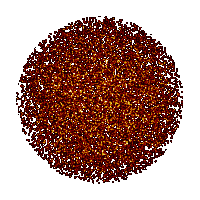
\includegraphics[width=0.49\textwidth]{images/reactor_design/htgr-mr-burn-200.inp_mesh1_bstep6.png}
   }
    \caption{Top-down view of the \gls{leup} X-Energy Xe-100 core model where darker shading corresponds to higher burnup, and lighter shading corresponds to lower burnup.}
    \label{fig:xe_core}
  \end{figure}

Figures \ref{fig:xe_init_core} and \ref{fig:xe_final_core} are shaded based on the burnup of the fuel, with darker pebbles indicating higher burnup. The pebbles are inserted into the core at the top, and gravity pulls them down through the core. After a brief holding time outside the core, the pebbles are reinserted at the top of the core. In \cyclus, we approximate the core as containing 6 batches in the core and one batch is removed when they reach the end of their life. This process is repeated until the pebbles reach their targeted number of passes, at which point they are removed from the core and stored.

\subsection{AP1000 Reactor}
\label{sec:ap}

AP1000s are operational in the \gls{usa} and China, and the \gls{uk} and India plan to deploy more. The Westinghouse AP1000 is a \gls{pwr} that uses UO$_2$ fuel. The reactor has an electrical output of 1000 MW, a cycle length such that every 18 months 80 fuel assemblies are replaced, and an expected lifetime of 60 years. The fuel is enriched to approximately 5\% $^{235}$U and has a discharge burnup of 65 GWd/MTU. The reactor in this thesis is an approximation based on publicly available data about the units currently operating at the Vogtle Plant in Georgia, and is not based on confidential or proprietary information. As this thesis does not anticipate \gls{leup} being used in the AP1000, there is no such neutronics model of the reactor herein, and this work adapts the generic \cycamore reactor archetype to represent the AP1000 in number of fuel assemblies, power output, core mass, and cycle length.



\chapter{Deployment Scenarios}
\label{ch:scenarios}
\glsresetall

In this chapter, we will discuss the transition scenarios for the deployment of new nuclear reactors in the \gls{usa} and the reactor models used in this work. We will also discuss the theoretical framework and key concepts that underpin the research, and the results for each deployment scheme.

\section{Transition Scenarios}
\label{sec:transition_scenarios}
% Discuss the theoretical framework and key concepts that underpin the research.

As the energy landscape evolves, compounding
factors will drive the actual deployment of these reactors in ways this work
does not capture. The value of energy system modeling and this type of
transition scenario is to understand the implications of deployment compared
with and measured relative to business-as-usual cases with similar
approximations.

We use this chapter to explore the deployment schemes we have
implemented---outlined in Table \ref{tab:deployment_schemes}---, and the demand
growth scenarios we have considered---outlined in Table
\ref{tab:demand_scenarios}. In Appendix \ref{sec:considered_deployment_schemes}
we will discuss two additional deployment schemes that we implemented, but
have not incorporated as they are more useful for problems not considered herein.

\begin{table}[H]
    \centering
    \caption{Deployment Schemes}
    \label{tab:deployment_schemes}
    \begin{tabular}{p{0.15\linewidth} p{0.27\linewidth} p{0.50\linewidth}}
        \hline
        \textbf{Status} & \textbf{Scheme} & \textbf{Description} \\
        \hline
        \multirow{4}{*}{Incorporated} & Greedy Deployment & Deploy the largest
        reactor first at each time step, fill in the remaining capacity with
        the next smallest, and so on. \\
        & Random Deployment & Uses a date and hour as seed to sample the
        reactors list randomly. \\
        & Initially Random, Greedy Deployment & Randomly deploys reactors until
        a reactor bigger than the remaining capacity is proposed for each time step,
        then fills the remaining capacity with the greedy algorithm. \\
        % & Single Reactor & A single reactor model is deployed as the existing fleet is decommissioned.\\
        \hline
        \multirow{2}{*}{Not Incorporated} & Capped Deployment & There is a
        single-number capacity for one or more of the reactor models. \\
        & Pre-Determined Distribution Deployment & One or more reactors have a
        preset distribution, and a smaller capacity model fills in the gaps. \\
        \hline
    \end{tabular}
\end{table}

We apply these deployment schemes to demand growth scenarios based on two
predictions of future energy demand. The \gls{eia} publishes demand expansion
projections for the totality of \gls{usa} \cite{eia_aeo_2023}. The
administration has refrained from publishing AEO 2024 in light of recent
accelerations in demand growth. Our assumptions for the low-growth scenarios
are that the relative percentage of nuclear power remains constant and that the
relative performance of the various fuel cycle metrics we simulate will remain
constant. Our high-growth scenarios come from the \gls{doe} Liftoff Report
\cite{julie_liftoff_pathways_2024}, which does not reflect this constant
percentage assumption for nuclear power in their demand scenarios. Their growth
projections are specific to nuclear deployment increases and the number is
agnostic to the total increase.

\begin{table}[H]
    \centering
    \caption{Demand Growth Scenarios}
    \label{tab:demand_scenarios}
    \begin{tabular}{c c c}
        \hline
        \textbf{Demand Growth} & \textbf{Year-to-Year Increase} & \textbf{Source}\\
        \hline
        No growth & 0\% & na\\
        Low growth & 0.17\%, 0.5\%, 1\%, & \cite{eia_aeo_2023}\\
        High growth & 3.5\%, 5.6\% & \cite{julie_liftoff_pathways_2024}\\
        \hline
    \end{tabular}
\end{table}

Each growth scenario is deployed under two regimes: 1) the reactors are never
fueled with \gls{leup}; 2) the \gls{mmr} and \gls{xe} reactors are fueled with
\gls{leup} until 2040, when they move to \gls{haleu}. \glspl{mmr} deployed
before this fuel transition will continue to use \gls{leup} fuel until the end
of their lifetime as they do not refuel; however, the \gls{xe} reactors will
refuel with \gls{leup} until 2040, when they will refuel with \gls{haleu}. The
AP1000 reactors will continue to use \gls{leu} fuel throughout the simulation.

Under each regime, each growth scenario is met by deploying reactors using the
schemes outlined in Table \ref{tab:deployment_schemes}. We will discuss the
results of these deployment schemes in the following sections. We will also
discuss the limitations of this work and propose future work. Regardless of the
regime, each deployment scheme will attempt to deploy reactors to meet the
capacity outlined in Figure \ref{fig:dep_goals}.

\begin{figure}[H]
    \centering
    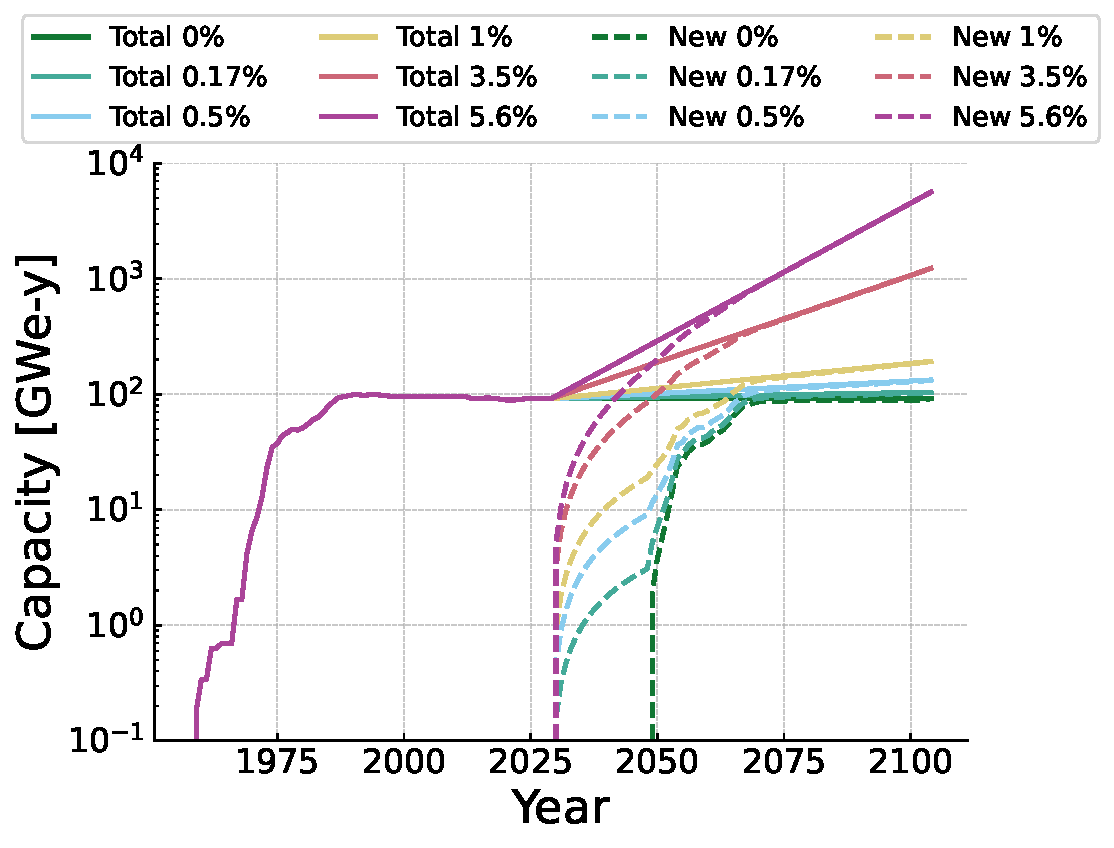
\includegraphics[scale=0.7]{images/results/deployment_calcs/total_new_capacity_scenarios.pdf}
    \caption{Total and new nuclear capacity deployed in each scenario}
    \label{fig:dep_goals}
\end{figure}

As shown, advanced reactors (for the purposes of this work the designs are the:
\gls{mmr}, \gls{xe}, and AP1000) begin deployment in 2030. While this is an
aggressive deployment schedule, \cite{bachmann_thesis_2023} established that
the precise deployment start did not significantly impact the total results for
this type of analysis and could reasonably serve as an upper bound of
deployment. The business-as-usual or, as we will refer to it, no growth
scenario does not require the deployment of a new nuclear reactor until just
before 2050, whereas the other scenarios understandably commence deployment in
2030. As we have presented the capacity on a logarithmic plot, the linear
appearance of the data belies the compounding effect that the year-to-year
percentage growth requires.

We will focus on the results of the no growth and $3.5\%$ (corresponding to a doubling of nuclear by 2050) scenarios, and the results for the other scenarios are available in Appendix \ref{ch:additional_results}.

\section{Metrics}
\label{sec:metrics}

% discuss the metrics you are using
In this work, we will develop a model of nuclear energy in the \gls{usa} using concepts from \glspl{esm} on scenarios that compare the transition from our current fleet to incorporate advanced reactor technologies not currently deployed. To compare these scenarios, we have chosen to focus on a few key metrics: \gls{swu}, energy output, mass of fuel, and reactor deployment.

\subsection{Separative Work Units}
\label{sec:swu}
% justify what swu is and why it is a valuable metric
The process of enriching uranium is a critical step in the nuclear fuel cycle, and, as we have highlighted, is expected to be a bottle neck in the deployment of advanced reactors. \gls{swu}, or a Separative Work Unit, is a ubiquitous measure of effort that goes into producing nuclear fuel. It is simplified as:
\begin{align}
    SWU&= (P \times V(x_p) + T \times V(x_t) - F \times V(x_f))\times t\nonumber
    V(x_i)&= (2 * x_i - 1) \times \ln\left(\frac{x_i}{1 - x_i}\right)\nonumber
    \intertext{Where:}
    SWU&= \mbox{Separative Work Units [kgSWU]}\nonumber\\
    P&= \mbox{Product mass flow rate [kg/d]}\nonumber\\
    F&= \mbox{Feed mass flow rate [kg/d]}\nonumber\\
    T&= \mbox{Tails mass flow rate [kg/d]}\nonumber\\
    V&= \mbox{Separation Potential [-]}\nonumber\\
    x_i&= \mbox{Weight fraction of $^{235}U$ in the i stream [-]}\nonumber\\
    x_p&= \mbox{Weight fraction of $^{235}U$ in the product stream [-]}\nonumber\\
    x_f&= \mbox{Weight fraction of $^{235}U$ in the feed stream [-]}\nonumber\\
    x_t&= \mbox{Weight fraction of $^{235}U$ in the tails stream [-]}\nonumber\\
    t&= \mbox{Time [d]}\nonumber
\end{align}

In this work, we will compare the \gls{swu} required for each scenario to understand the relative effort required to deploy the reactors and provide a stable precursor to economic calculations. As we mention in Section \ref{sec:leup}, the definition used in the literature for \gls{leup} can be tied to the upper limit on enrichment for a Category III facility. The \gls{leup} fuel, as shown in Table \ref{tab:ar_defs}, is enriched to 9.95\% $^{235}$U, which would fall under the Category III limit. The \gls{haleu} fuel would require Category II facilities to achieve the 19.75\% $^{235}$U and 15.5\% $^{235}$U enrichment for the \gls{mmr} and \gls{xe} \gls{haleu}respectively. The \gls{swu} required for each scenario will be compared to understand the relative effort required to deploy the reactors and provide a stable precursor to economic calculations.

In Table

\begin{table}
    \centering
    \caption{SWU calculation values for each fuel type}
    \label{tab:swu_vals}
    \begin{tabular}{c c}
        \hline
        \textbf{Variable} & \textbf{Value}\\
        \hline
        \gls{mmr} \gls{leup} $x_p$ & 0.0995\\
        \gls{mmr} \gls{haleu} $x_p$ & 0.1975\\
        \gls{xe} \gls{leup} $x_p$ & 0.0995\\
        \gls{xe} \gls{haleu} $x_p$ & 0.155\\
        \gls{leu} $x_p$ & 0.045\\
        $x_f$ & 0.00711\\
        $x_t$ & 0.002\\
        \hline
    \end{tabular}
\end{table}

\subsection{Energy Output}
\label{sec:energy_output}

The deployment of reactors in this work is based on energy demand, which
approximates the complicated relationship that generators and utilities
have with power expansions. The reactors simulated herein have a static peak energy output, so the nuance in the fleet's ability to meet the demand comes from the deployment scheme and limitations in the fuel supply chain. We will devote time to discussing the realistic features of each scheme. \cyclus tracks the energy output of each reactor, and we will compare that with the demand scenarios to understand the relative performance of each deployment scheme.


\subsection{Mass of Fuel}
\label{sec:mass_of_fuel}

\cyclus tracks the mass of material in each transaction, in this work we will characterize the deployment challenge ahead of us using the fresh and used fuel accumulation to show the relative mass of fuel required to deploy the reactors in each scenario. From the mass of fuel, and knowledge of the fuel design, these results can be converted into cost metrics, transportation modeling, and hypothetical repository space considerations.

\section{Greedy Deployment}
\label{sec:greedy_deployment}

In this scheme, we deploy the largest reactor first until another
deployment of that reactor exceeds the demand---as outlined in
\ref{fig:greedy_diagram}. Then we move to the next largest reactor until the
next deployment of the smallest capacity reactor exceeds the
demand. This scheme is not a proxy for strategic decisions by individual
actors it merely meets the demand in a roughly efficient manner.

Previous work from Bachmann et al. \cite{bachmann_enrichment_2021}
employed a similar scheme to explore the deployment of advanced
reactors in the \gls{usa}. This scheme is computationally efficient and allows
for the exploration of the deployment of advanced reactors in a way that is not
overly complex. This scheme is most useful for scenarios where the user is
interested in comparing metrics relative to the number of specific reactors
deployed outside of the context of the problem.

\begin{figure}[H]
    \centering
    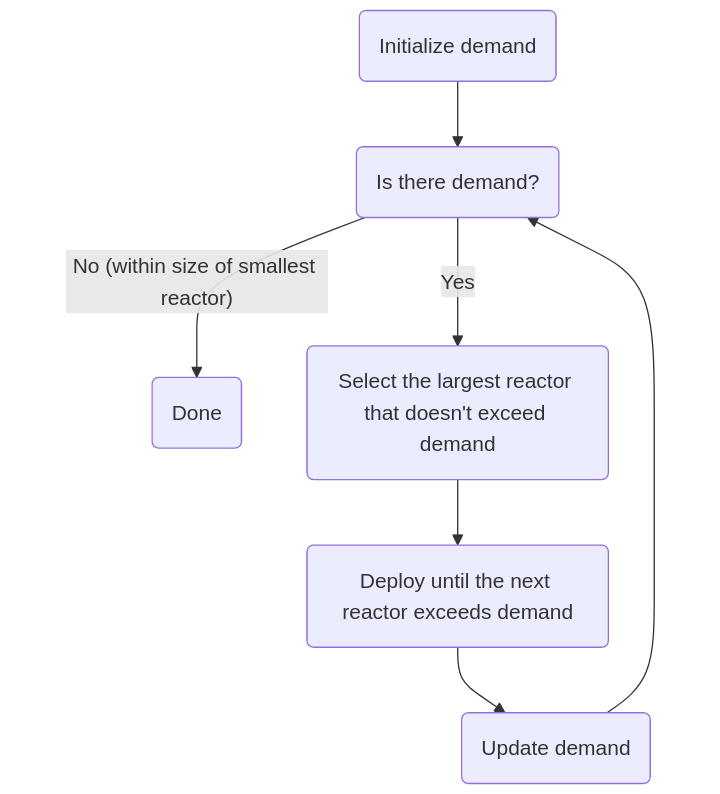
\includegraphics[scale=0.3]{images/schemes/greedy_diagram.png}
    \caption{Greedy deployment diagram.}
    \label{fig:greedy_diagram}
\end{figure}

Through the greedy deployment, we are not attempting to capture the complexity
of the deployment problem but rather to explore the implications of deploying a
certain number of reactors. As such, we limit the discussion of realism to the
extent that the scheme meets the demand and could mirror large actors in a
market. The scheme will deploy reactors until the demand is met within the
amount of the smallest capacity reactor. In these results, we will show the results for the no growth scenario and the double nuclear by 2050 scenario.

\subsection{Number of Reactors}
\label{sec:greedy_reactors}

As we have noted, one of the most notable differences between the no growth scenario and the doubling scenario is that the transition for the no growth scenario will begin closer to 2050 instead of 2030. This trend is reflected in Figures \ref{fig:greedy_mf_reactors} and \ref{fig:greedy_of_reactors}, where the \glspl{mmr}, \glspl{xe}, and AP1000s start as the existing \gls{lwr} fleet are retired. Comparing across fuel regimes, we see that Figures \ref{fig:greedy_mf_ng_reactors} and \ref{fig:greedy_of_ng_reactors} are identical, which typifies the impact of the delayed transition in the no growth scenario.

% Show total number of reactors multi fuel

\begin{figure}[H]
    \subfloat[No Growth. \label{fig:greedy_mf_ng_reactors}]{%
      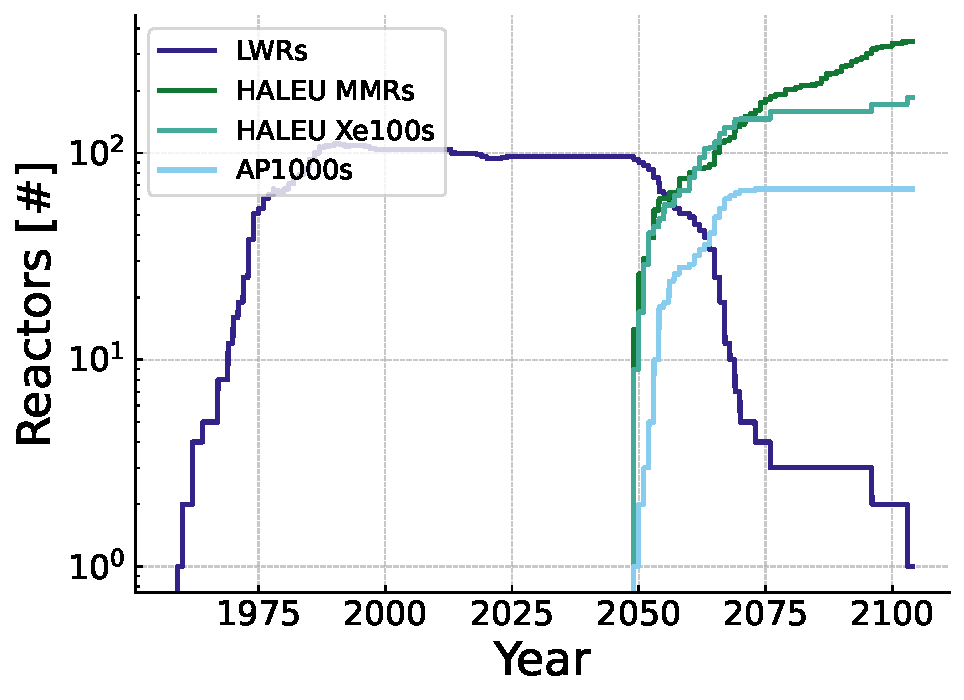
\includegraphics[width=0.495\textwidth]{images/results/reactors/multi_dgng_reactors.pdf}
   }
    \hfill
    \subfloat[Double. \label{fig:greedy_mf_d2_reactors}]{%
      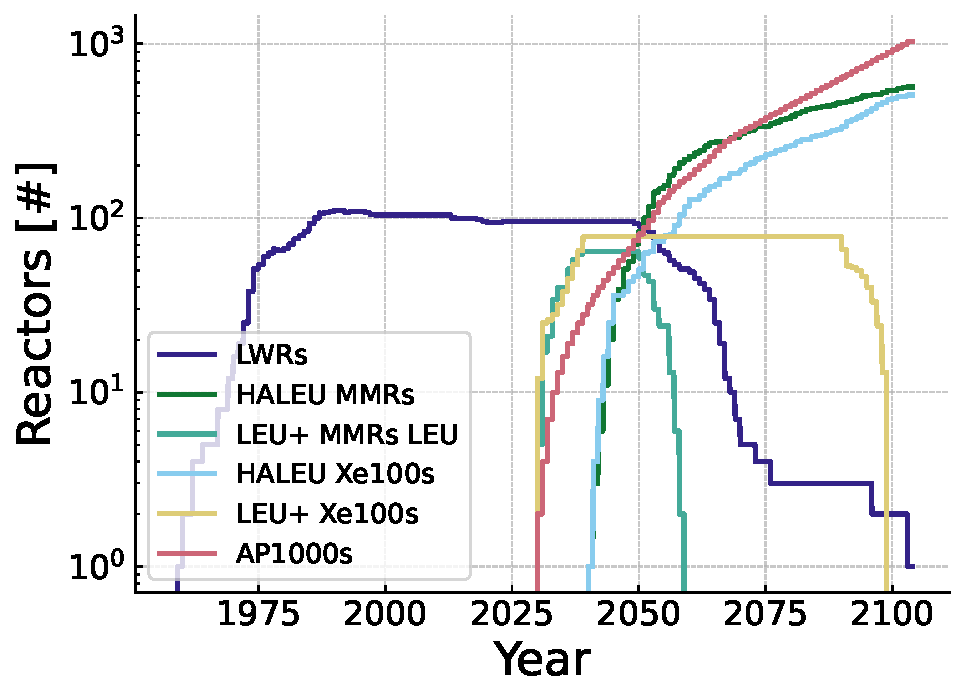
\includegraphics[width=0.495\textwidth]{images/results/reactors/multi_dg2_reactors.pdf}
   }
    \caption{Greedy multi fuel reactor deployment.}
    \label{fig:greedy_mf_reactors}
\end{figure}

% talk about the rate of deployment
A direct consequence of the greedy deployment scheme is that, in the doubling scenario, the AP1000 is deployed the most over time, where as the no growth scenario shows the opposite. Another consequence of the deployment scheme is that the rate of deployment for the single fuel regime compared with the multi fuel regime is identical, and future work could investigate further implications of transitioning from one fuel type to another in regard to operation. Simply meeting energy demand is not how utilities make decisions, and is not the intended use case of the broad generation of new nuclear reactors, so we are able to identify an upper bounding case for the energy demand met by designs like the \gls{mmr} or \gls{xe}.


\begin{figure}[H]
  \subfloat[No Growth. \label{fig:greedy_of_ng_reactors}]{%
    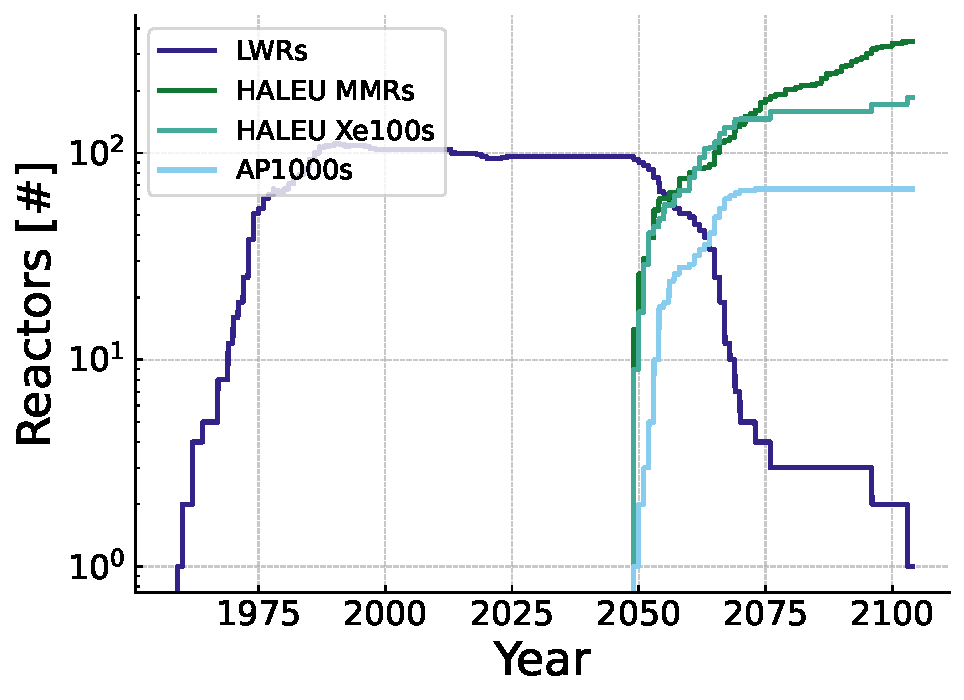
\includegraphics[width=0.495\textwidth]{images/results/reactors/one_dgng_reactors.pdf}
 }
  \hfill
  \subfloat[Double. \label{fig:greedy_of_d2_reactors}]{%
    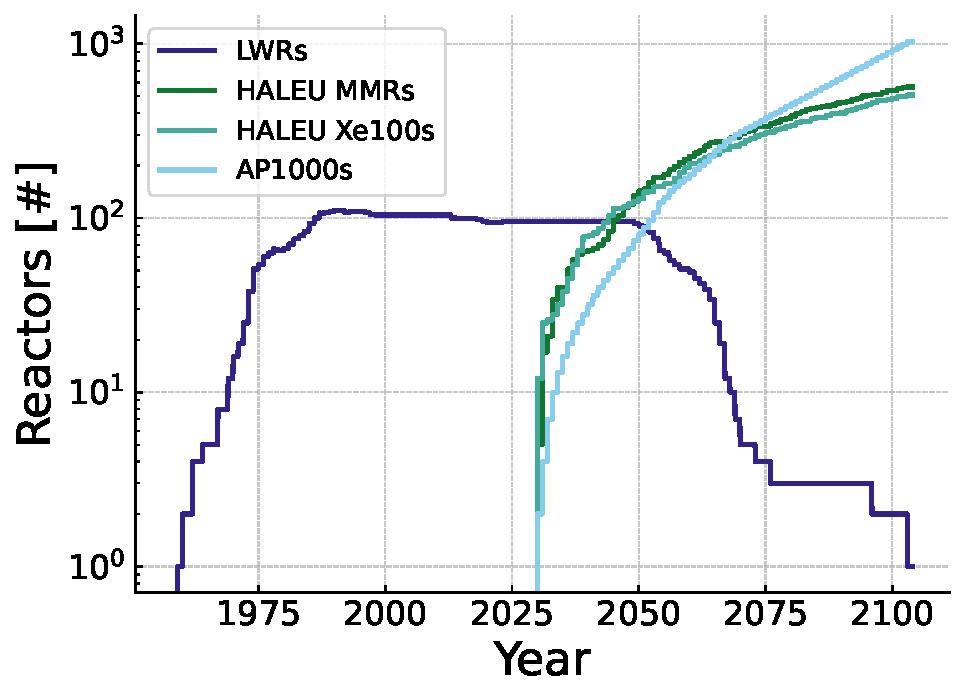
\includegraphics[width=0.495\textwidth]{images/results/reactors/one_dg2_reactors.pdf}
 }
  \caption{Greedy single fuel reactor deployment.}
  \label{fig:greedy_of_reactors}
\end{figure}

In Table \ref{tab:greedy_reac_avg} we can see how the average number of reactors by design is not influenced by the interstitial as we have modeled it in this work. Compared to the no growth scenario, the double by 2050 scenario shows a significant increase in the average number of each design operating across the 2030-2104 timeline. Consequently, the average number of the AP1000s increases by 757\% between the two growth scenarios, which is the largest increase of any design. The \gls{xe} reactors show the second largest increase at 163\%, followed by the \gls{mmr} at 109\%.

\begin{table}[H]
  \centering
  \caption{Average greedy total operating reactors by design.}
  \label{tab:greedy_reac_avg}
  \begin{tabular}{c c c c c}
     \hline
     Scenario & No Growth, Single & No Growth, Multiple & Double, Single & Double, Multiple  \\
     \hline
     \gls{haleu} fueled MMRs      & 131.613 & 131.613 & 274.493 & 257.427 \\
     \gls{leup} fueled MMRs       & --      & --      & --      & 17.067 \\
     \gls{haleu} fueled \gls{xe}s & 94.04   & 94.04   & 246.88  & 184.48 \\
     \gls{leup} fueled \gls{xe}s  & --      & --      & --      & 62.4 \\
     \gls{leu} fueled AP1000      & 38.667  & 38.667  & 331.387 & 331.387 \\
     \hline
  \end{tabular}
\end{table}




\subsection{SWU Results}
\label{sec:greedy_swu}

% talk about the types of category facility
In Figure \ref{fig:swu_yearly_greedy} we can see the yearly \gls{swu} demand
periodically spike as the demand for enrichment services grows to meet the fuel
demand for the fleet. When reactors begin operation in the depicted no growth
scenario around 2050, the \gls{swu} demand for the AP1000 peaks above the other
two reactors while the demand from \glspl{xe} exceeds the demand from
\glspl{mmr}. This trend is exacerbated in the double by 2050 scenarios shown in
Figures \ref{fig:greedy_mf_d2_swu} and \ref{fig:greedy_of_d2_swu} where the
\gls{swu} for AP1000 \gls{leu} fuel rises quickly and eventually exceeds the
total \gls{swu} for the existing fleet.

% talk about the SWU capacity

% show the total SWU capacity

\begin{figure}[H]
    \centering
    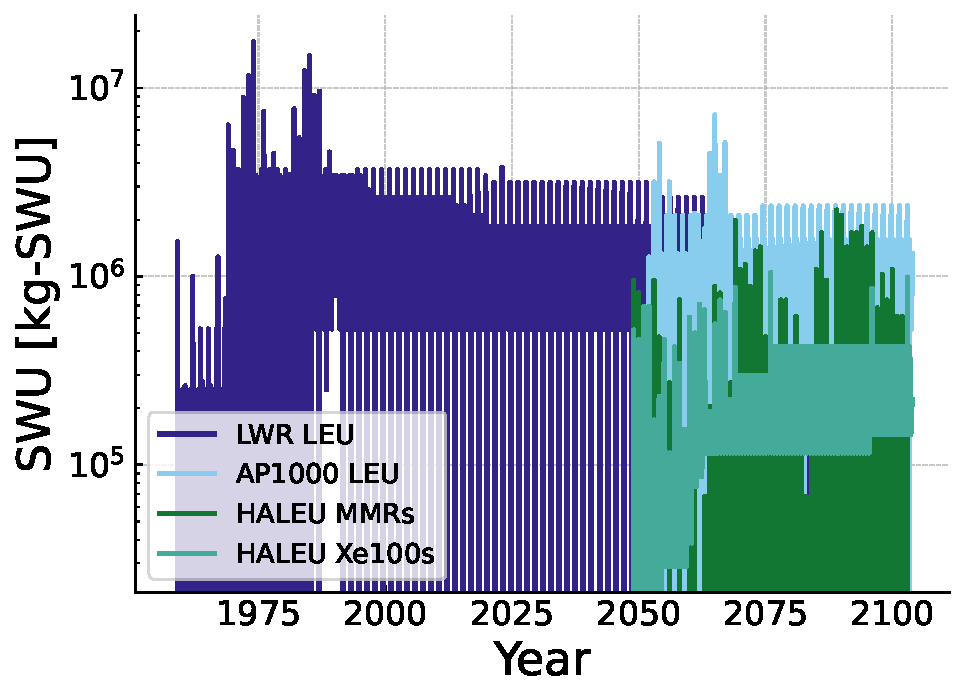
\includegraphics[scale=0.7]{images/results/swu/multi_dgng_swu_by_fuel.pdf}
    \caption{Greedy yearly SWU capacity multi fuel, no growth scenario.}
    \label{fig:swu_yearly_greedy}
\end{figure}

As the features of the yearly data are regular and dictated by the cycles of the reactors, we will visualize the total \gls{swu} demand in the cumulative plots in Figures \ref{fig:greedy_mf_swu} and \ref{fig:greedy_of_swu}.

\begin{figure}[H]
  \subfloat[No Growth. \label{fig:greedy_mf_ng_swu}]{%
    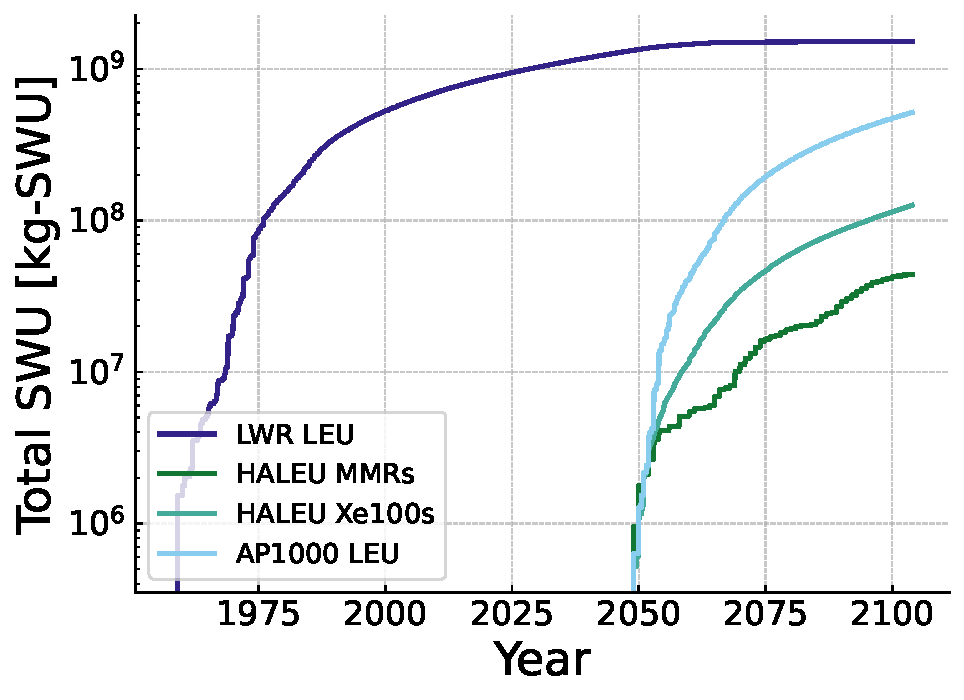
\includegraphics[width=0.495\textwidth]{images/results/swu/multi_dgng_swu_cumulative_by_fuel.pdf}
 }
  \hfill
  \subfloat[Double. \label{fig:greedy_mf_d2_swu}]{%
    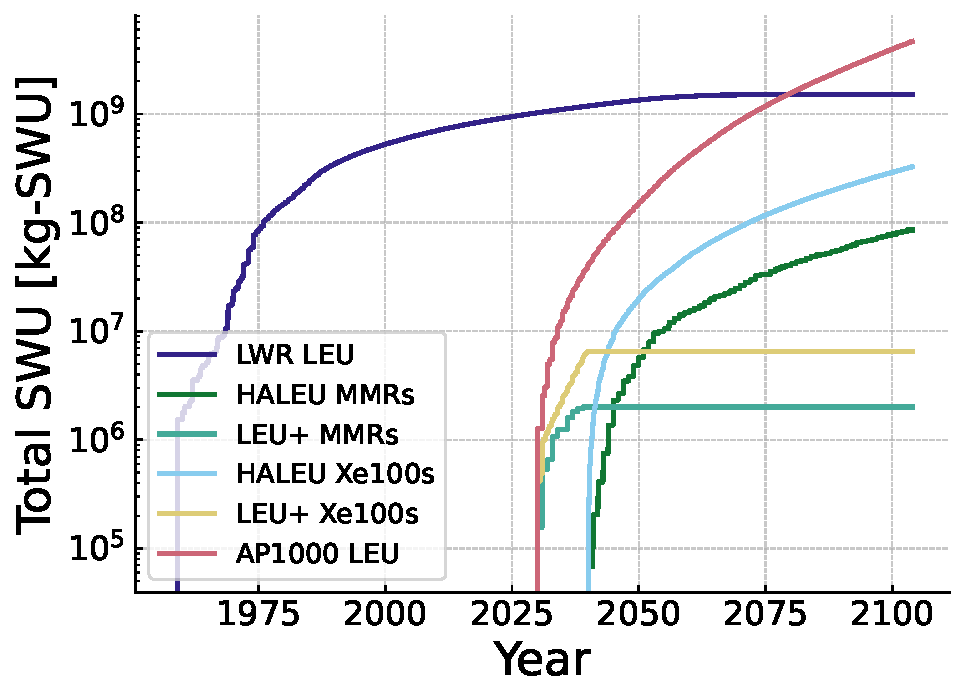
\includegraphics[width=0.495\textwidth]{images/results/swu/multi_dg2_swu_cumulative_by_fuel.pdf}
 }
  \caption{Greedy multi fuel SWU.}
  \label{fig:greedy_mf_swu}
\end{figure}


% talk about international trade

\begin{figure}[H]
  \subfloat[No Growth. \label{fig:greedy_of_ng_swu}]{%
    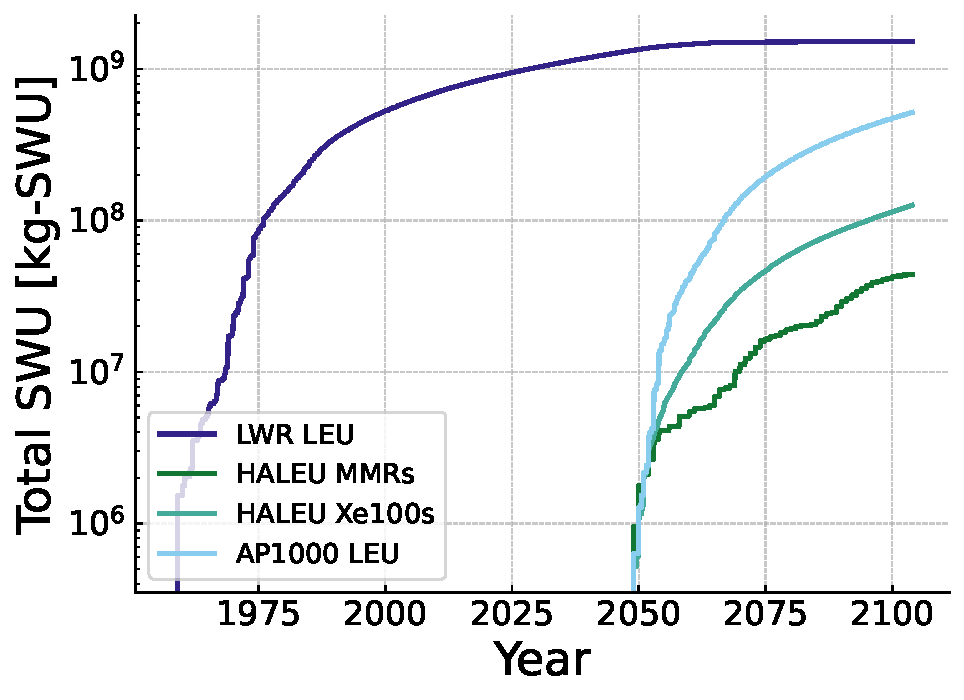
\includegraphics[width=0.495\textwidth]{images/results/swu/one_dgng_swu_cumulative_by_fuel.pdf}
 }
  \hfill
  \subfloat[Double. \label{fig:greedy_of_d2_swu}]{%
    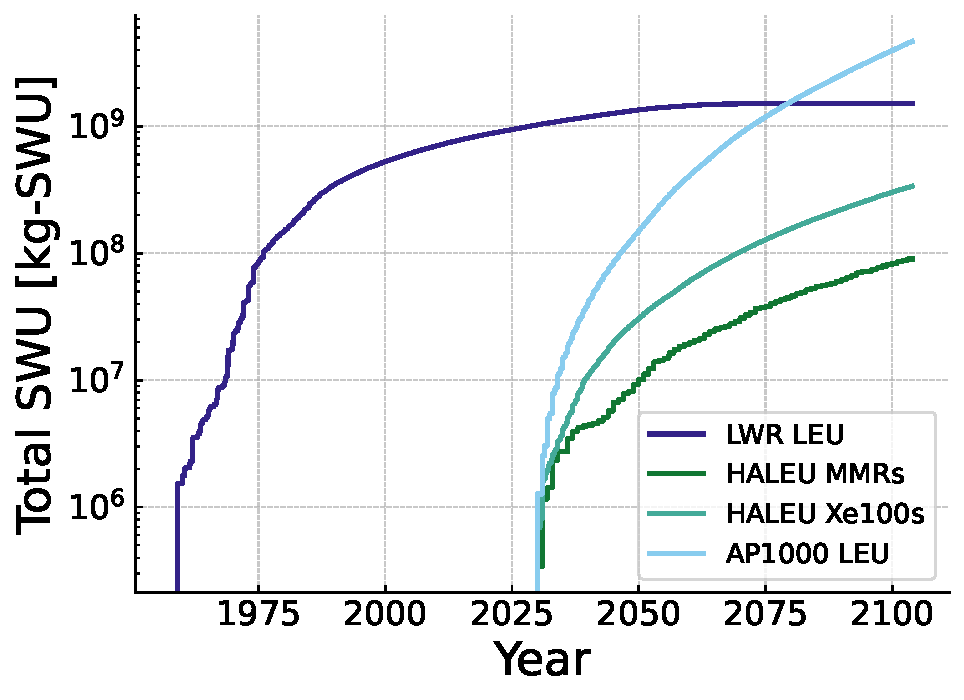
\includegraphics[width=0.495\textwidth]{images/results/swu/one_dg2_swu_cumulative_by_fuel.pdf}
 }
  \caption{Greedy single fuel SWU.}
  \label{fig:greedy_of_swu}
\end{figure}

In Table \ref{tab:greedy_swu_avg} we can see the average \gls{swu} demand by design in the no growth and double by 2050 scenarios. The \gls{swu} demand for the \gls{mmr} and \gls{xe} reactors is the same in the single and multi fuel regimes for the no growth scenarios, which is consistent with the reactor deployment trends we have seen in the Section \ref{sec:greedy_reactors}. The \gls{swu} demand for the AP1000s increases by 800\% from the no growth scenario to the double scenario, which is consistent with the reactor deployment trends we have seen in the previous section. The \gls{swu} demand for \gls{xe} \gls{haleu} increases 167\%, while the \gls{swu} demand for \gls{mmr} \gls{haleu} increases 105\% from the no growth scenario to the double scenario.

\begin{table}[H]
  \centering
  \caption{Average greedy yearly SWU by design in k\gls{swu}.}
  \label{tab:greedy_swu_avg}
  \begin{tabular}{c c c c c}
     \hline
     Scenario & No Growth, Single & No Growth, Multiple & Double, Single & Double, Multiple  \\
     \hline
     \gls{mmr} \gls{haleu}   & 48.699  & 48.699  & 99.974   & 95.127   \\
     \gls{mmr} \gls{leup}    & --      & --      & --       & 2.228    \\
     \gls{xe} \gls{haleu}    & 139.926 & 139.926 & 374.323  & 362.312  \\
     \gls{xe} \gls{leup}     & --      & --      & --       & 7.227    \\
     AP1000 \gls{leu}        & 573.989 & 573.989 & 5167.815 & 5167.815 \\
     \hline
  \end{tabular}
\end{table}



\subsection{Fresh Fuel Results}
\label{sec:greedy_fresh}

% talk about the types of fuel
In Figures \ref{fig:greedy_mf_fresh} and \ref{fig:greedy_of_fresh} we can see the fresh fuel demand for the reactors in the no growth and double by 2050 scenarios. The fresh fuel curves in each scenario follow the same pattern as the reactor deployment curves, as \cyclus supplies fuel to each of the reactors as it is deployed.

% show total fresh fuel

\begin{figure}[H]
  \subfloat[No Growth. \label{fig:greedy_mf_ng_fresh}]{%
    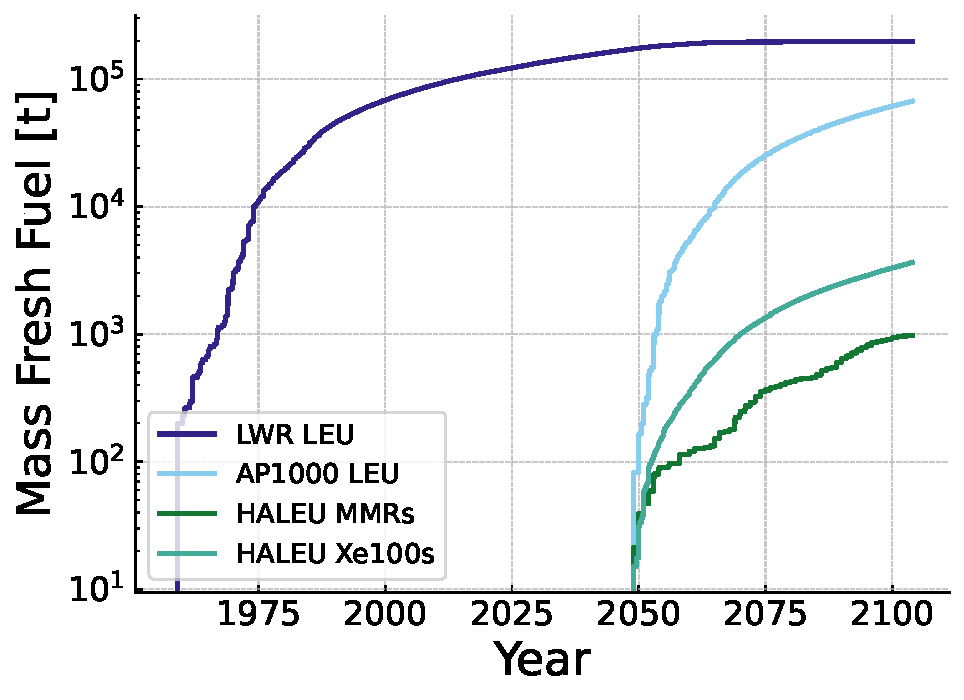
\includegraphics[width=0.495\textwidth]{images/results/fresh/multi_dgng_fresh_fuel_cumulative_by_fuel.pdf}
 }
  \hfill
  \subfloat[Double. \label{fig:greedy_mf_d2_fresh}]{%
    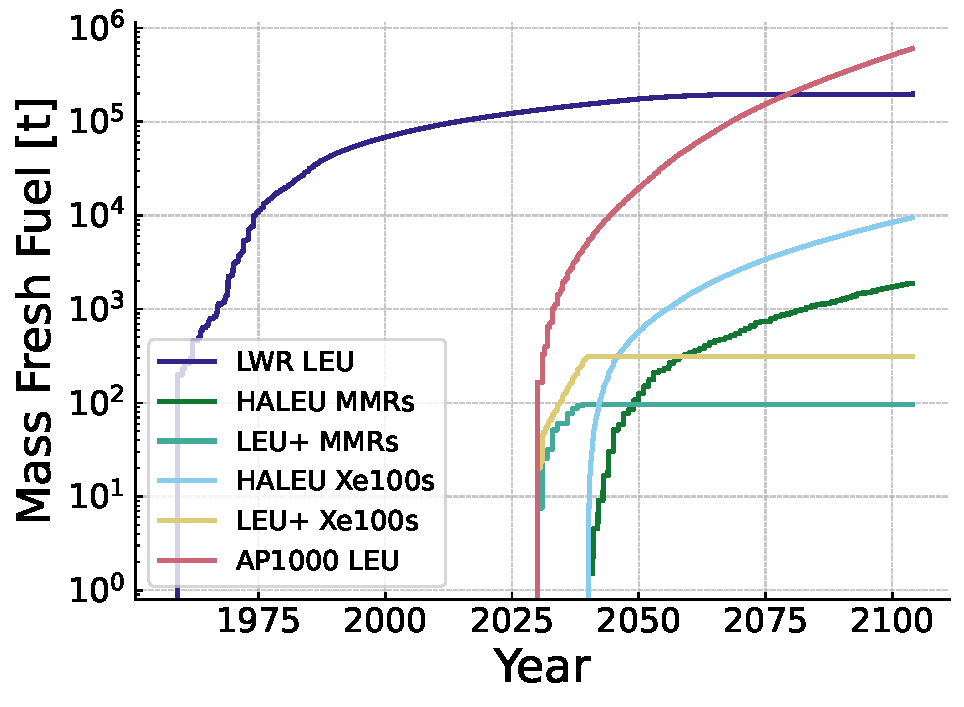
\includegraphics[width=0.495\textwidth]{images/results/fresh/multi_dg2_fresh_fuel_cumulative_by_fuel.pdf}
 }
  \caption{Greedy multi fresh fuel demanded.}
  \label{fig:greedy_mf_fresh}
\end{figure}

% talk about transportation of fuel


\begin{figure}[H]
  \subfloat[No Growth. \label{fig:greedy_of_ng_fresh}]{%
    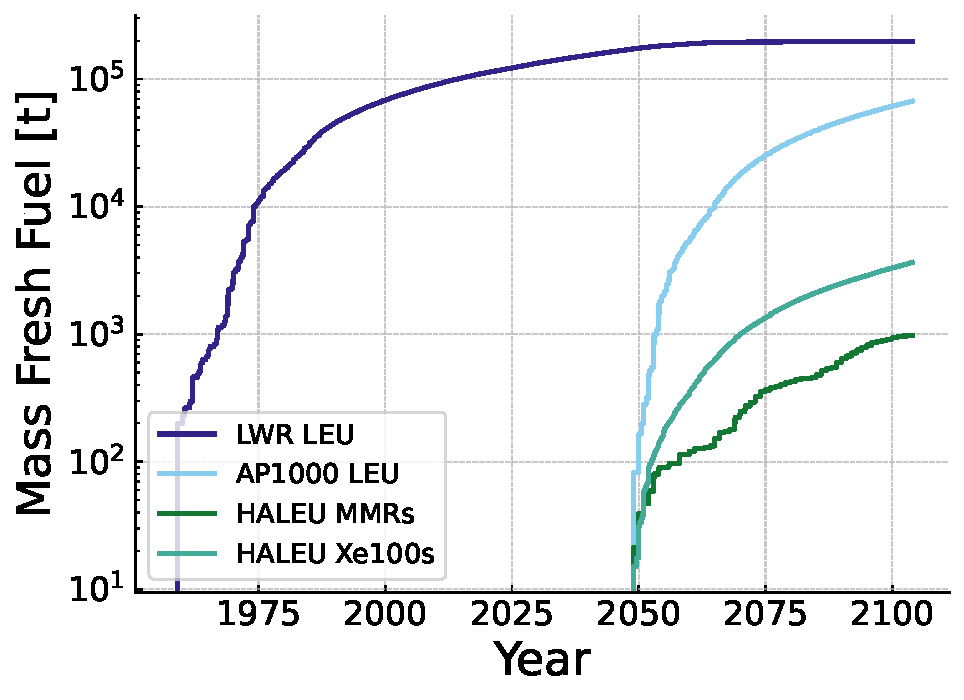
\includegraphics[width=0.495\textwidth]{images/results/fresh/one_dgng_fresh_fuel_cumulative_by_fuel.pdf}
 }
  \hfill
  \subfloat[Double. \label{fig:greedy_of_d2_fresh}]{%
    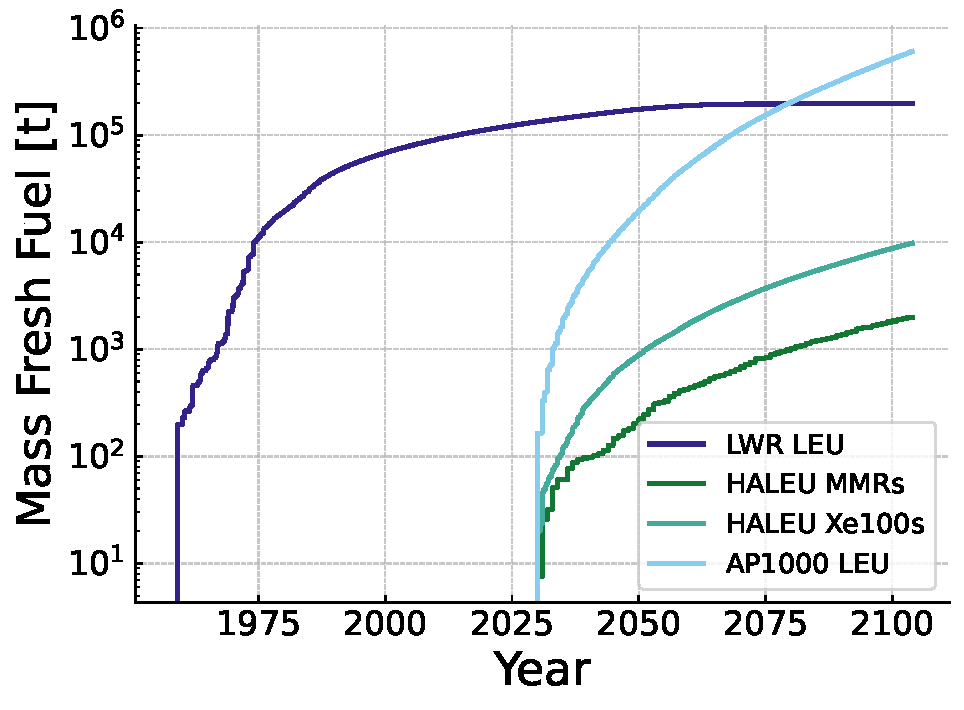
\includegraphics[width=0.495\textwidth]{images/results/fresh/one_dg2_fresh_fuel_cumulative_by_fuel.pdf}
 }
  \caption{Greedy single fresh fuel demanded.}
  \label{fig:greedy_of_fresh}
\end{figure}

In Table \ref{tab:greedy_fresh_avg} we can see the average yearly fresh fuel demand by design in the no growth and double by 2050 scenarios. The AP1000 \gls{leu} shows the largest increase in fresh fuel demand from the no growth scenario to the double scenario at 800\%, followed by the \gls{xe} \gls{haleu} at 159\%. The \gls{mmr} \gls{haleu} reactors show the smallest increase in fresh fuel demand at 105\%.


\begin{table}[H]
  \centering
  \caption{Average greedy yearly fresh fuel by design in tonnes.}
  \label{tab:greedy_fresh_avg}
  \begin{tabular}{c c c c c}
     \hline
     Scenario & No Growth, Single & No Growth, Multiple & Double, Single & Double, Multiple  \\
     \hline
     \gls{mmr} \gls{haleu}   & 1.079    & 1.079   & 2.216    & 2.108    \\
     \gls{mmr} \gls{leup}    & --       & --      & --       & 0.107    \\
     \gls{xe} \gls{haleu}    & 4.059    & 4.059   & 10.859   & 10.511   \\
     \gls{xe} \gls{leup}     & --       & --      & --       & 0.348    \\
     AP1000 \gls{leu}        & 74.636   & 74.636  & 671.976  & 671.976  \\
     \hline
  \end{tabular}
\end{table}



\subsection{Used Fuel Results}
\label{sec:greedy_used}

In Figures \ref{fig:greedy_mf_used} and \ref{fig:greedy_of_used} we can see the used fuel demand for the reactors in the no growth and double by 2050 scenarios. The used fuel curves in each scenario lag the reactor deployment curves, as \cyclus removes the used fuel after the appropriate number of cycles from  each of the operating, and eventually decommissioning, reactors.

% show total used fuel
\begin{figure}[H]
  \subfloat[No Growth. \label{fig:greedy_mf_ng_used}]{%
    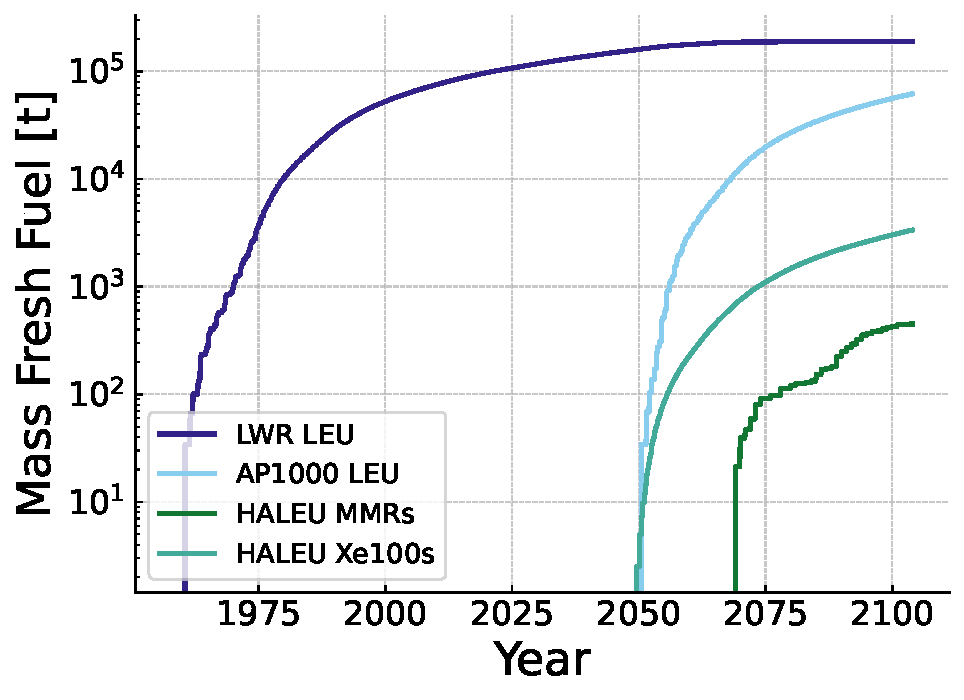
\includegraphics[width=0.495\textwidth]{images/results/used/multi_dgng_used_fuel_cumulative_by_fuel.pdf}
 }
  \hfill
  \subfloat[Double. \label{fig:greedy_mf_d2_used}]{%
    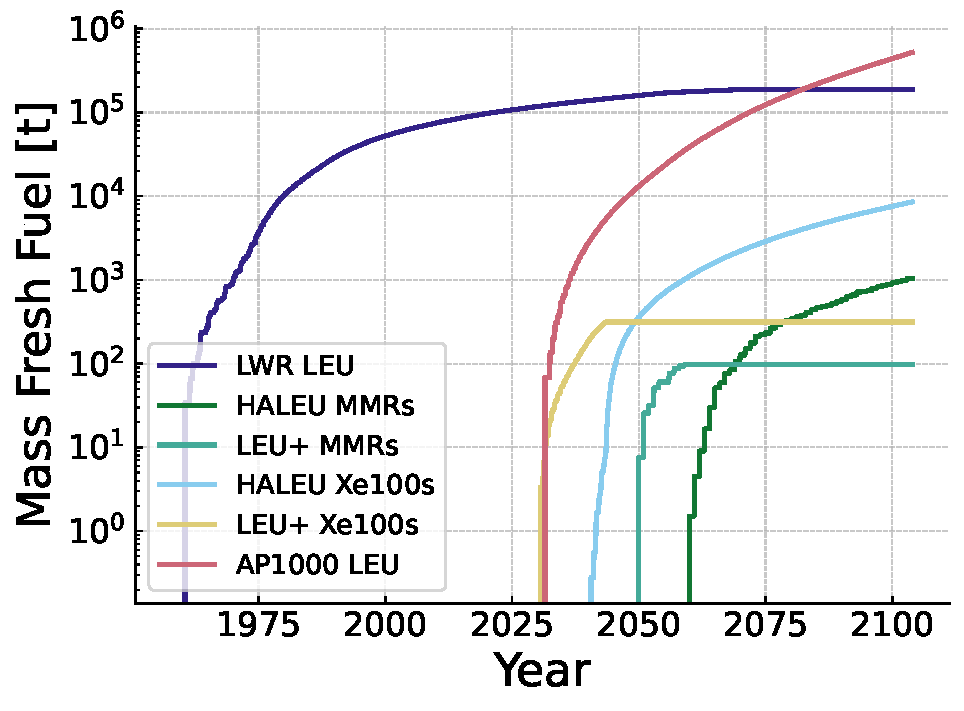
\includegraphics[width=0.495\textwidth]{images/results/used/multi_dg2_used_fuel_cumulative_by_fuel.pdf}
 }
  \caption{Greedy multi used fuel accumulation.}
  \label{fig:greedy_mf_used}
\end{figure}


\begin{figure}[H]
  \subfloat[No Growth. \label{fig:greedy_of_ng_used}]{%
    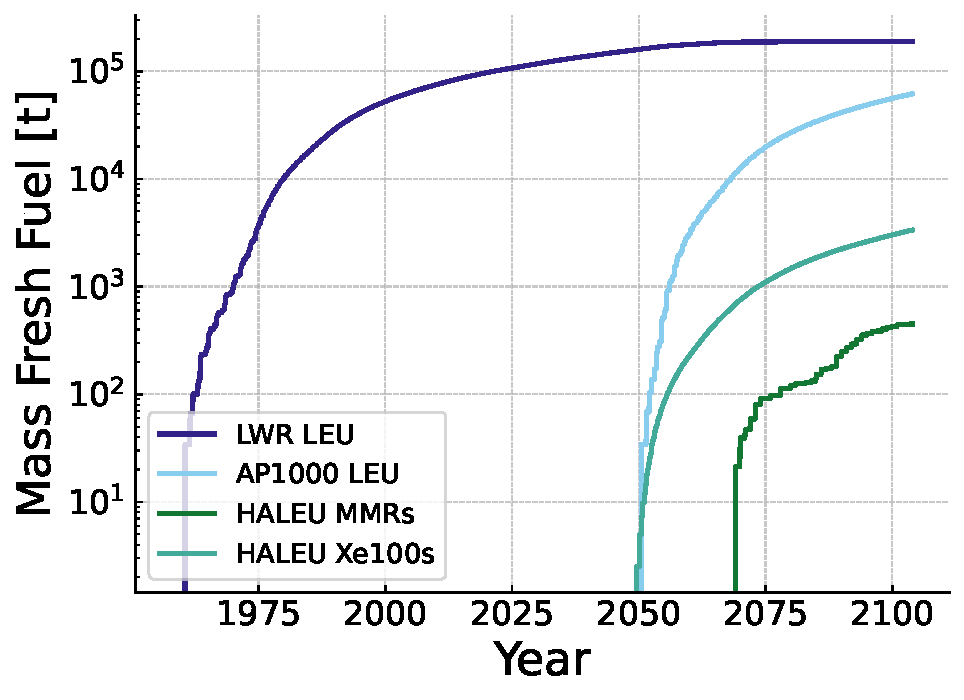
\includegraphics[width=0.495\textwidth]{images/results/used/one_dgng_used_fuel_cumulative_by_fuel.pdf}
 }
  \hfill
  \subfloat[Double. \label{fig:greedy_of_d2_used}]{%
    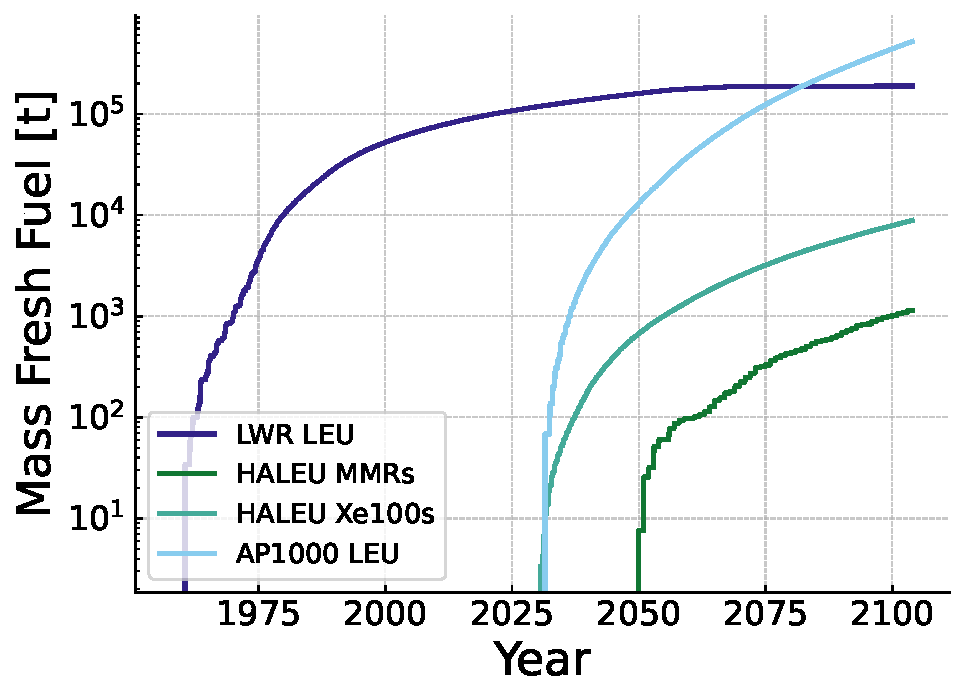
\includegraphics[width=0.495\textwidth]{images/results/used/one_dg2_used_fuel_cumulative_by_fuel.pdf}
 }
  \caption{Greedy single used fuel accumulation.}
  \label{fig:greedy_of_used}
\end{figure}

In Table \ref{tab:greedy_used_avg} we can see the average yearly used fuel by design in the no growth and double by 2050 scenarios. The AP1000 \gls{leu} shows the largest increase in used fuel demand from the no growth scenario to the double scenario at 743\%, followed by the \gls{xe} \gls{haleu} at 164\%. The \gls{mmr} \gls{haleu} reactors show the smallest increase in used fuel demand at 154\%.


\begin{table}[H]
  \centering
  \caption{Average greedy yearly used fuel by design in tonnes.}
  \label{tab:greedy_used_avg}
  \begin{tabular}{c c c c c}
     \hline
     Scenario & No Growth, Single & No Growth, Multiple & Double, Single & Double, Multiple  \\
     \hline
     \gls{mmr} \gls{haleu}   & 0.499    & 0.499   & 1.267    & 1.160    \\
     \gls{mmr} \gls{leup}    & --       & --      & --       & 0.107    \\
     \gls{xe} \gls{haleu}    & 3.714    & 3.715   & 9.826    & 9.477    \\
     \gls{xe} \gls{leup}     & --       & --      & --       & 0.348    \\
     AP1000 \gls{leu}        & 68.496   & 68.496  & 577.484  & 577.484  \\
     \hline
  \end{tabular}
\end{table}


% talk about repositories

\section{Random Deployment}
\label{sec:random_deployment}

Advanced reactor concepts, like the ones outlined in this work, are often
designed for use cases ranging from industrial steam production to microgrid
integration. Our deployment of these reactors is
a complex problem that requires a nuanced understanding of the energy market,
the regulatory environment, the intended use of the technology, and the
technical capabilities of the reactor.

This random deployment is a proxy for the complexity of the real-world
deployment problem but does not include the nuance of how individual
deployments meet an end user's needs, which will drive the strategic decisions
that utilities and ratepayers behind the meter make in their reactor choices
The random deployment scheme has the potential to capture some of the
complexities in overall market development, but the extent we capture these
details is not explored in this work.

The random deployment scheme is implemented by randomly selecting reactors from
the list of deployable reactors until the demand is covered. We illustrate this
scheme in Figure \ref{fig:random_diagram}, which shows the single loop in the
logic from the top down. There is an irreducible demand that cannot be met
because the power capacity is assumed to be constant. As such the random
deployment scheme, at its best, will meet the demand, but has the potential to
fall short of the demand by one of the smallest capacity reactors. To reduce
the computational cost of this scheme, we have implemented a rough random case
that deploys until the randomly selected reactor exceeds the demand. This rough
approximation is what we couple with the greedy deployment scheme in the
initially random, greedy deployment scheme in Section
\ref{sec:initially_random_greedy}.

\begin{figure}[H]
    \centering
    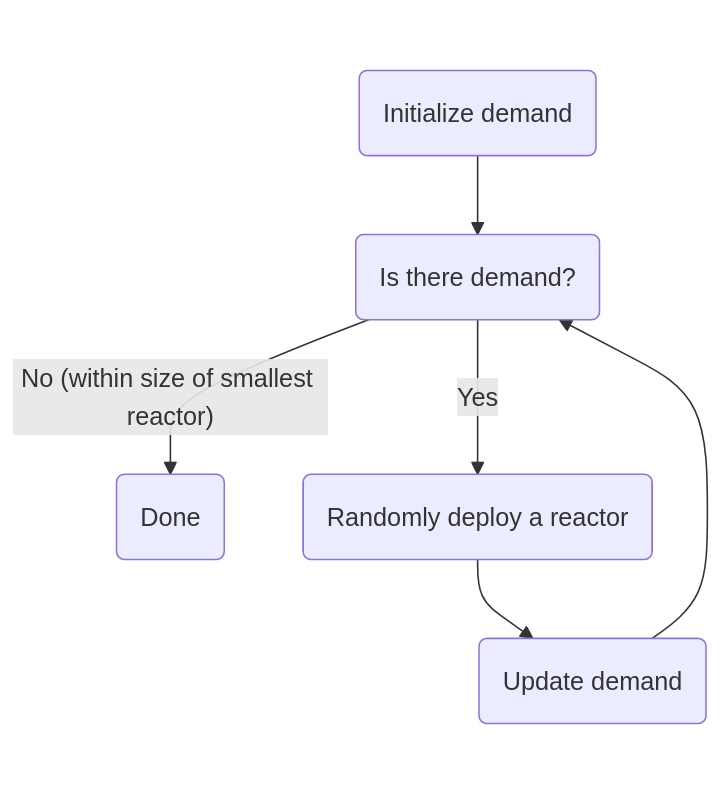
\includegraphics[scale=0.3]{images/schemes/random_diagram.png}
    \caption{Random Deployment Diagram}
    \label{fig:random_diagram}
\end{figure}

The seed, which was set to 20240527121205 for every run for this scheme, for
the random number generator is set by the date and time of the simulation,
which allows for the reproducibility of the results. This scheme is a proxy for
aggregate decisions by actors and would fail to reliably capture individual
actor decisions. This scheme is most useful for scenarios or timescales where
there is a high degree of uncertainty in the deployment of reactors.


\subsection{Number of Reactors}
\label{sec:random_reactors}

As we discussed in Section \ref{sec:greedy_reactors}, the difference between the no growth and double scenarios in Figures \ref{fig:random_mf_reactors} and \ref{fig:random_of_reactors} is that the double scenario requires new reactors to be deployed immediately at the transition. A consequence of the random reactor deployment scheme is that the number of reactors in Figure \ref{fig:random_mf_ng_reactors} and \ref{fig:random_mf_d2_reactors} grow similarly over time as they are sampled for deployment. This scheme has the potential to stochastically capture the complexity of deploying reactors in the real world, but likely represents an extreme where utilities are not narrowing in on a single reactor design to reduce costs of deployment.

% Show total number of reactors multi fuel
\begin{figure}[H]
    \subfloat[No Growth \label{fig:random_mf_ng_reactors}]{%
      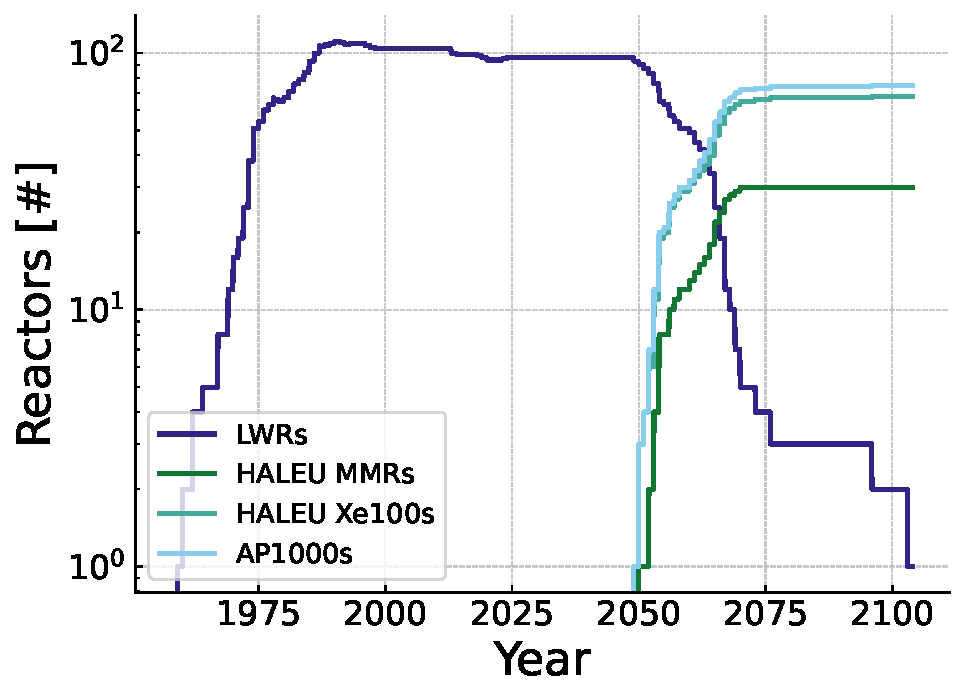
\includegraphics[width=0.495\textwidth]{images/results/reactors/multi_drng_reactors.pdf}
   }
    \hfill
    \subfloat[Double \label{fig:random_mf_d2_reactors}]{%
      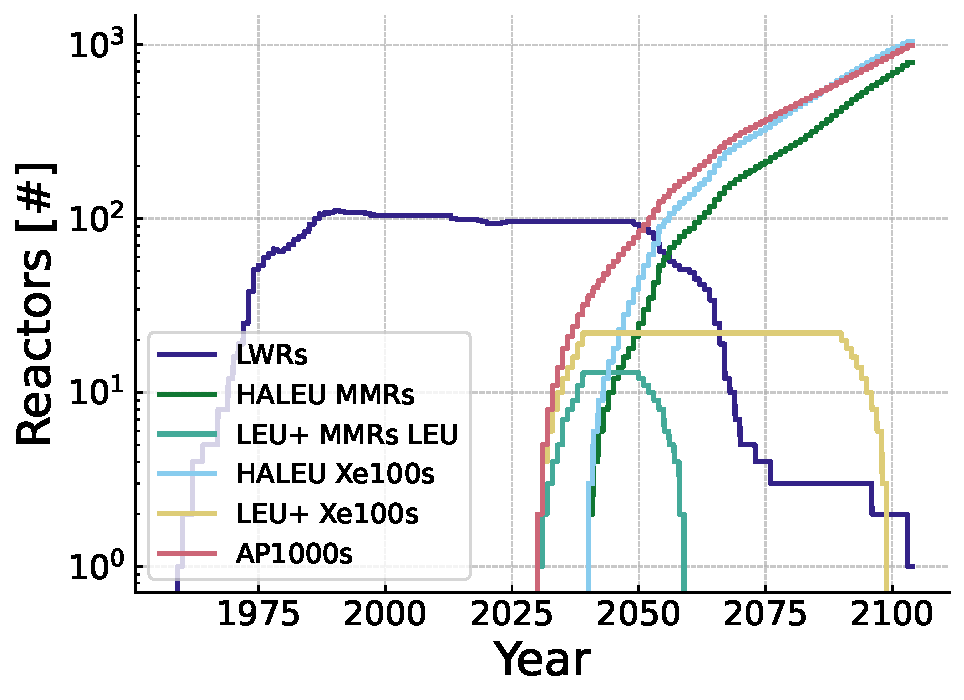
\includegraphics[width=0.495\textwidth]{images/results/reactors/multi_dr2_reactors.pdf}
   }
    \caption{Multiple fuels random reactor deployment.}
    \label{fig:random_mf_reactors}
  \end{figure}

% talk about the rate of deployment

% talk about the context of expanding energy needs

% talk about the workers

\begin{figure}[H]
    \subfloat[No Growth \label{fig:random_of_ng_reactors}]{%
      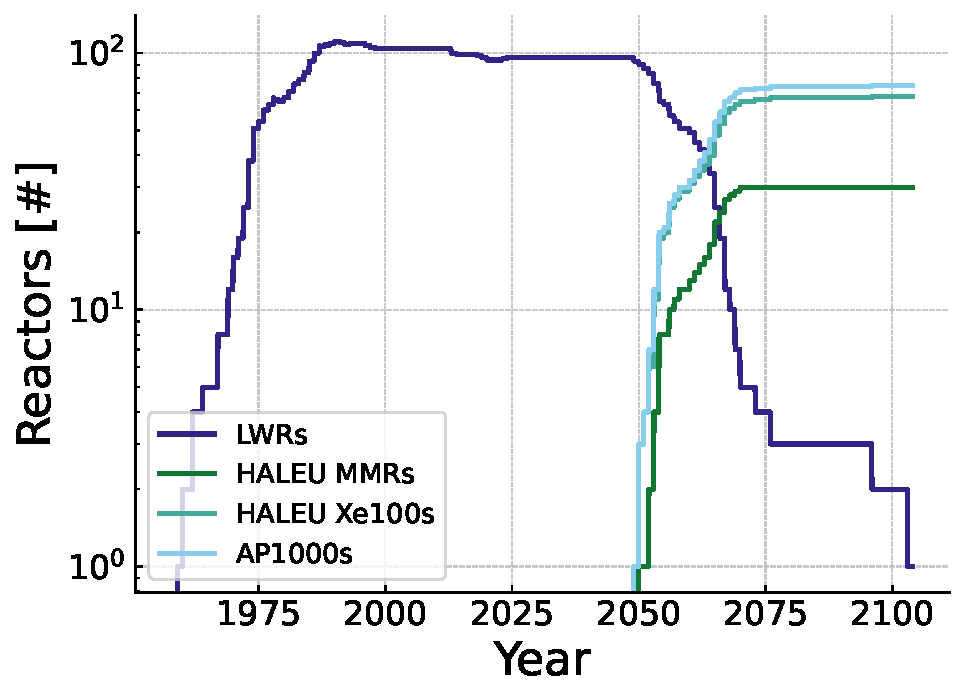
\includegraphics[width=0.495\textwidth]{images/results/reactors/one_drng_reactors.pdf}
   }
    \hfill
    \subfloat[Double \label{fig:random_of_d2_reactors}]{%
      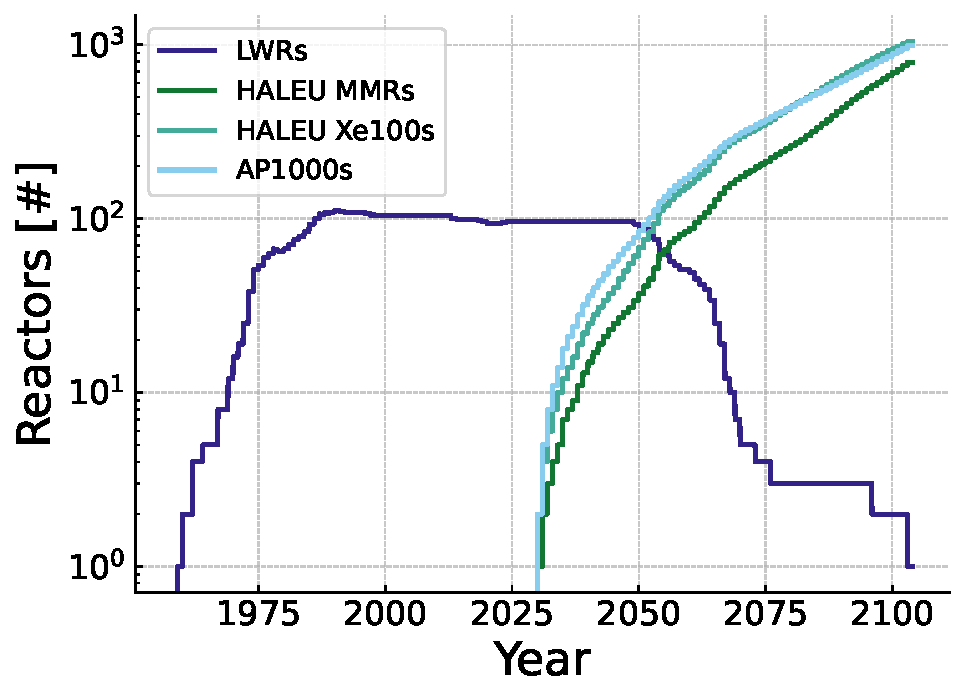
\includegraphics[width=0.495\textwidth]{images/results/reactors/one_dr2_reactors.pdf}
   }
    \caption{Single fuel random reactor deployment.}
    \label{fig:random_of_reactors}
  \end{figure}


In Table \ref{tab:random_reac_avg}, we show the average total number of reactors for the no growth and double scenarios in the single and multi fuel regimes. There is a 740\% increase in the number of AP1000s deployed going from the no growth scenario to the double scenario. The \gls{xe} reactors show a 249\% increase, while the \gls{mmr} reactors show a 62\% increase in the number of reactors deployed going from the no growth scenario to the double scenario in the single fuel regime. Unlike the reactor deployment under the greedy scheme in Section \ref{sec:greedy_reactors} and the initially random then greedy scheme in Section \ref{sec:rand_greed_reactors}, the random deployment scheme results for the single fuel and multi fuel regimes are not the same.

In the multi fuel regime, the AP1000 reactors show a 660\% increase in the number of reactors deployed going from the no growth scenario to the double scenario. The \gls{xe} reactors show a 746\% increase, while the \gls{mmr} reactors show a 1138\% increase in the number of reactors deployed going from the no growth scenario to the double scenario.

\begin{table}[H]
    \centering
    \caption{Average random total operating reactors by design.}
    \label{tab:random_reac_avg}
    \begin{tabular}{c c c c c}
       \hline
       Scenario & No Growth, Single & No Growth, Multiple & Double, Single & Double, Multiple  \\
       \hline
       \gls{haleu} fueled \glspl{mmr} & 131.613 & 17.267  & 213.707 & 210.24  \\
       \gls{leup} fueled \glspl{mmr}  & --      & --      & --      & 3.467   \\
       \gls{haleu} fueled \glspl{xe}  & 94.04   & 38.813  & 328.173 & 310.573 \\
       \gls{leup} fueled \glspl{xe}   & --      & --      & --      & 17.6    \\
       \gls{leu} fueled AP1000s       & 38.667  & 42.72   & 324.68  & 324.68  \\
       \hline
    \end{tabular}
\end{table}




\subsection{SWU Results}
\label{sec:random_swu}

In Figure \ref{fig:swu_yearly_random} we can see the yearly \gls{swu} demand periodically spike as reactors begin operation in the depicted no growth scenario around 2050. The \gls{swu} demand for the AP1000 \gls{leu} rises above the other two reactors while the demand from \glspl{xe} overlaps heavily with the demand from \glspl{mmr}. This trend is exacerbated in the double by 2050 scenarios shown in Figures \ref{fig:greedy_mf_d2_swu} and \ref{fig:greedy_of_d2_swu} where the \gls{swu} for AP1000 \gls{leu} fuel rises quickly and eventually exceeds the total \gls{swu} for the existing fleet.


% talk about the SWU capacity

% show the total SWU capacity
\begin{figure}[H]
    \centering
    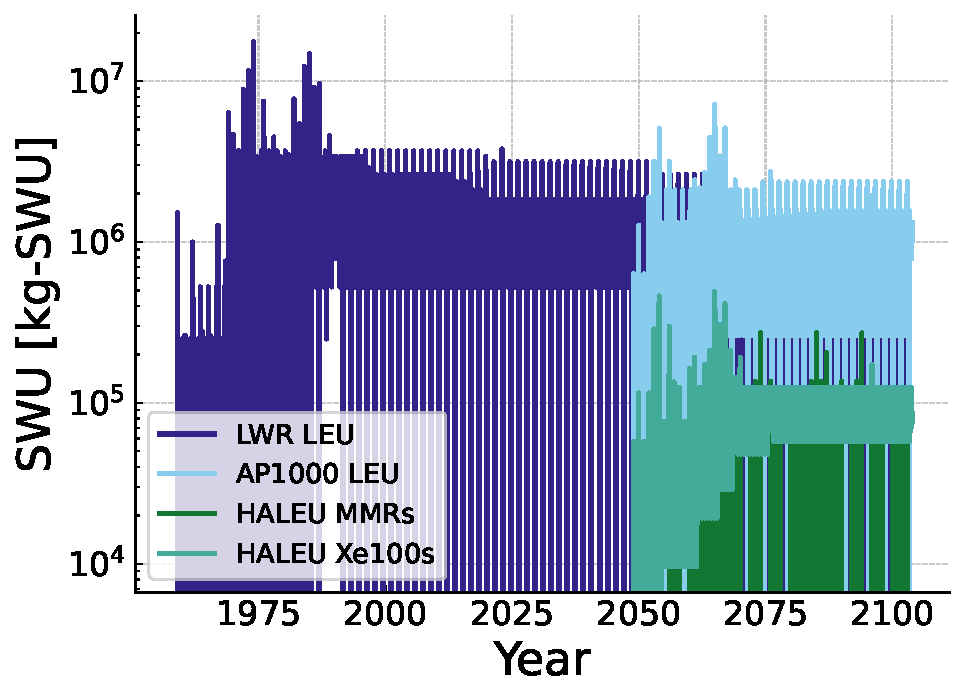
\includegraphics[scale=0.7]{images/results/swu/multi_drng_swu_by_fuel.pdf}
    \caption{Random reactor yearly SWU capacity.}
    \label{fig:swu_yearly_random}
\end{figure}

As the features of the yearly data are regular, dictated by the cycles of the
reactors, and overlapping, we will visualize the total \gls{swu} demand in the
cumulative plots in Figures \ref{fig:random_mf_swu} and \ref{fig:random_of_swu}.


\begin{figure}[H]
  \subfloat[No Growth \label{fig:random_mf_ng_swu}]{%
    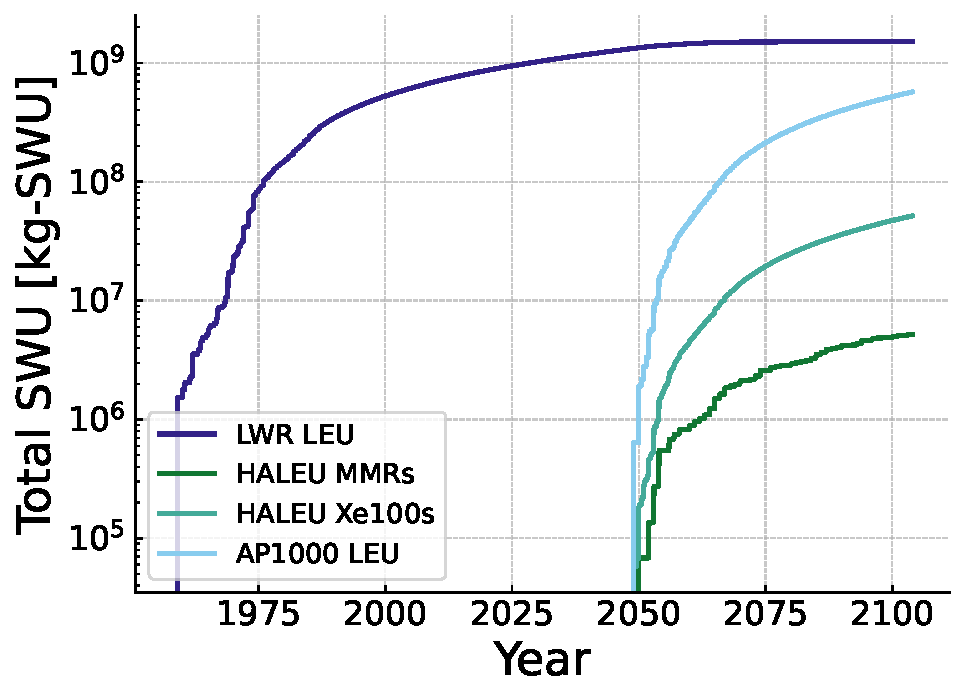
\includegraphics[width=0.495\textwidth]{images/results/swu/multi_drng_swu_cumulative_by_fuel.pdf}
 }
  \hfill
  \subfloat[Double \label{fig:random_mf_d2_swu}]{%
    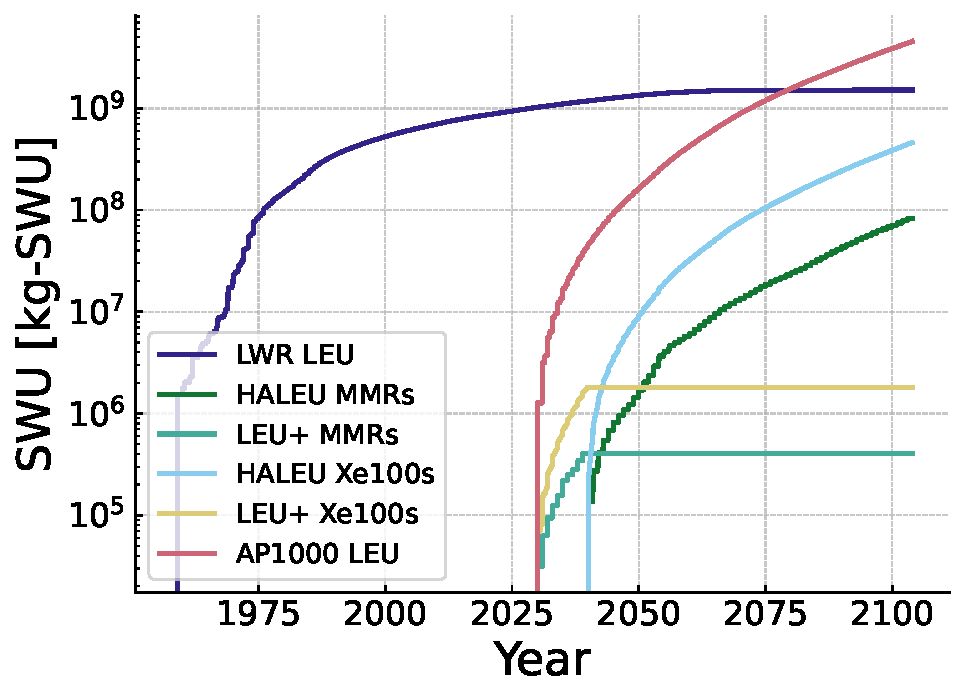
\includegraphics[width=0.495\textwidth]{images/results/swu/multi_dr2_swu_cumulative_by_fuel.pdf}
 }
  \caption{Random reactor multi fuel SWU.}
  \label{fig:random_mf_swu}
\end{figure}

% talk about international trade

\begin{figure}[H]
    \subfloat[No Growth \label{fig:random_of_ng_swu}]{%
      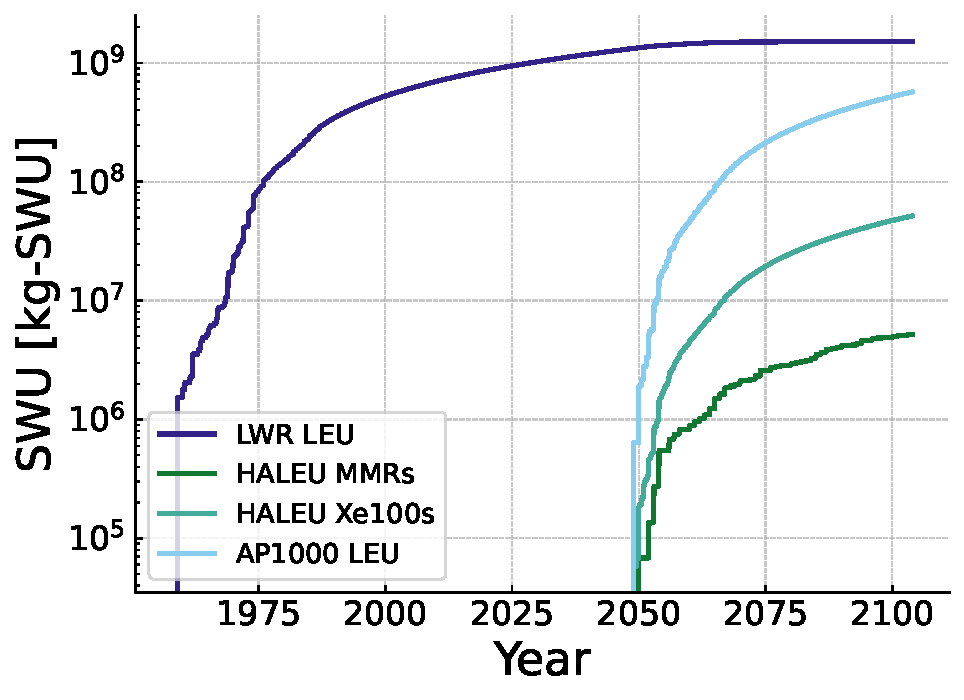
\includegraphics[width=0.495\textwidth]{images/results/swu/one_drng_swu_cumulative_by_fuel.pdf}
   }
    \hfill
    \subfloat[Double \label{fig:random_of_d2_swu}]{%
      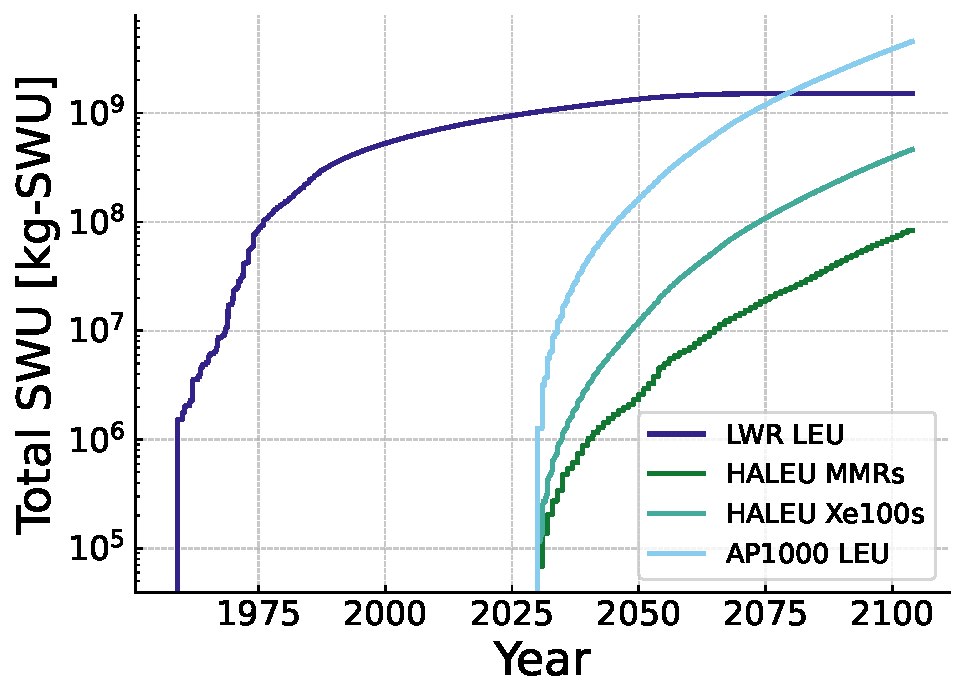
\includegraphics[width=0.495\textwidth]{images/results/swu/one_dr2_swu_cumulative_by_fuel.pdf}
   }
    \caption{Random reactor single fuel SWU.}
    \label{fig:random_of_swu}
\end{figure}


In Table \ref{tab:random_swu_avg}, we show the average total yearly \gls{swu} capacity for the no growth and double scenarios in the single and multi fuel regimes under the random deployment scheme. The \gls{xe} reactors show a 796\% increase in the average total yearly \gls{swu} capacity going from the no growth scenario to the double scenario in the single fuel regime. The \gls{mmr} reactors show a 1511\% increase in the average total yearly \gls{swu} capacity going from the no growth scenario to the double scenario in the single fuel regime. The AP1000 reactors show a 697\% increase in the average total yearly \gls{swu} capacity going from the no growth scenario to the double scenario in the single fuel regime.

\begin{table}[H]
    \centering
    \caption{Average random yearly SWU by design in tonnes of \gls{swu}.}
    \label{tab:random_swu_avg}
    \begin{tabular}{c c c c c}
       \hline
       Scenario & No Growth, Single & No Growth, Multiple & Double, Single & Double, Multiple  \\
       \hline
       \gls{mmr} \gls{haleu}   & 5.756   & 5.756   & 92.703    & 91.719   \\
       \gls{mmr} \gls{leup}    & --      & --      & --       & 0.453    \\
       \gls{xe} \gls{haleu}    & 57.327  & 57.327  & 513.746  & 510.388  \\
       \gls{xe} \gls{leup}     & --      & --      & --       & 2.021    \\
       AP1000 \gls{leu}        & 634.554 & 634.554 & 5050.323 & 5050.323 \\
       \hline
    \end{tabular}
\end{table}





\subsection{Fresh Fuel Results}
\label{sec:random_fresh}

% talk about the types of fuel
In Figures \ref{fig:random_mf_fresh} and \ref{fig:random_of_fresh} we can see the fresh fuel demand for the reactors in the no growth and double by 2050 scenarios. The fresh fuel curves in each scenario follow the same pattern as the reactor deployment curves from Figures \ref{fig:random_mf_reactors} and \ref{fig:random_of_reactors}, as \cyclus supplies fuel to each of the reactors as it they deploy.

% show total fresh fuel

\begin{figure}[H]
    \subfloat[No Growth \label{fig:random_mf_ng_fresh}]{%
      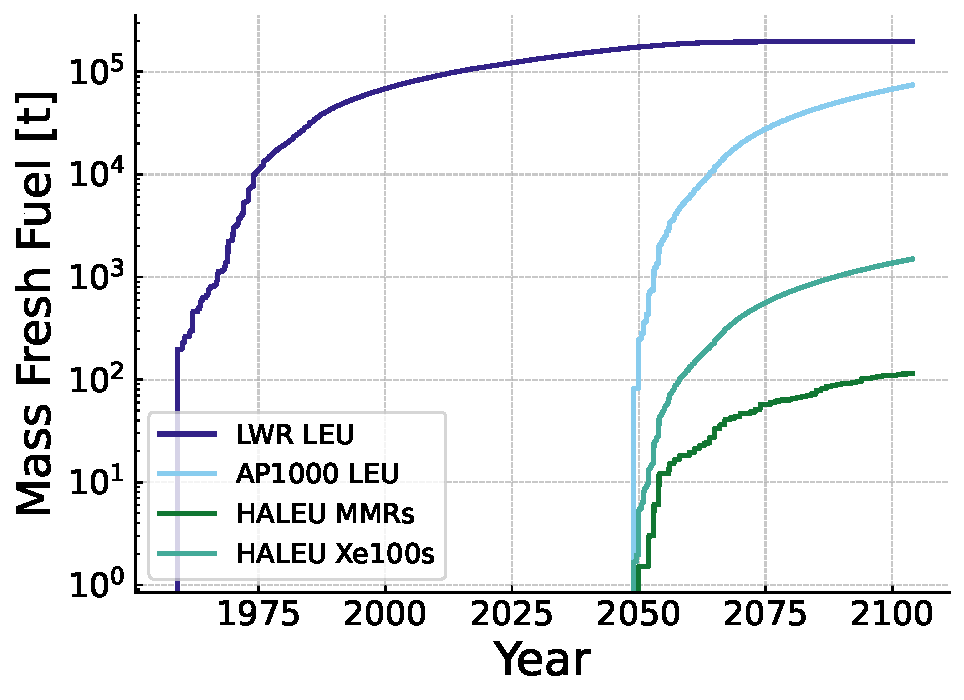
\includegraphics[width=0.495\textwidth]{images/results/fresh/multi_drng_fresh_fuel_cumulative_by_fuel.pdf}
   }
    \hfill
    \subfloat[Double \label{fig:random_mf_d2_fresh}]{%
      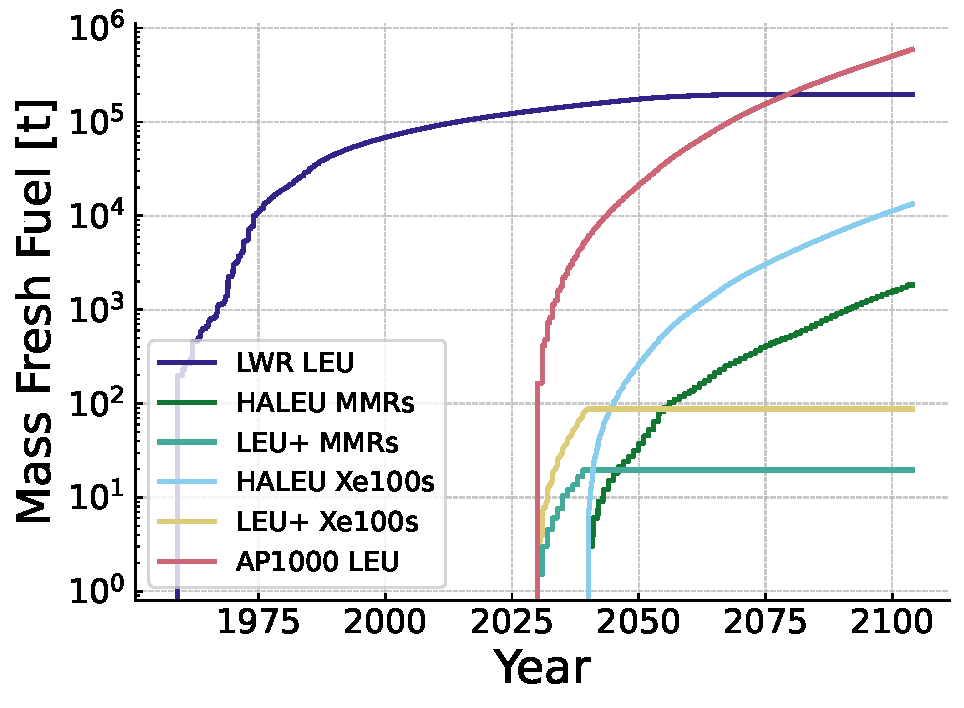
\includegraphics[width=0.495\textwidth]{images/results/fresh/multi_dr2_fresh_fuel_cumulative_by_fuel.pdf}
   }
    \caption{Random multi fresh fuel demanded.}
    \label{fig:random_mf_fresh}
  \end{figure}

% talk about transportation of fuel


\begin{figure}[H]
    \subfloat[No Growth \label{fig:random_of_ng_fresh}]{%
      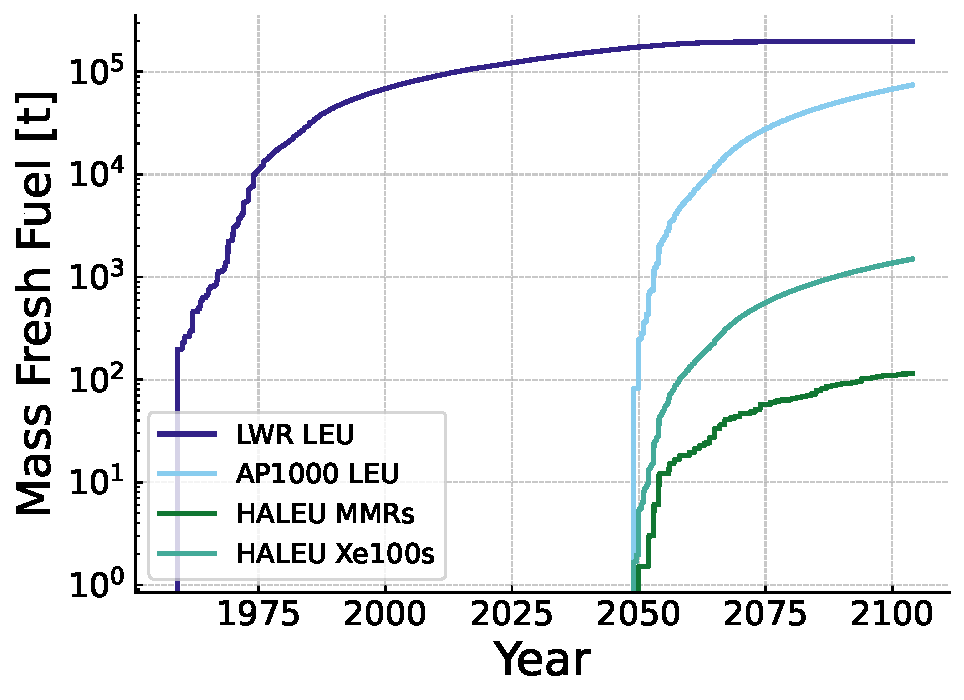
\includegraphics[width=0.495\textwidth]{images/results/fresh/one_drng_fresh_fuel_cumulative_by_fuel.pdf}
   }
    \hfill
    \subfloat[Double \label{fig:random_of_d2_fresh}]{%
      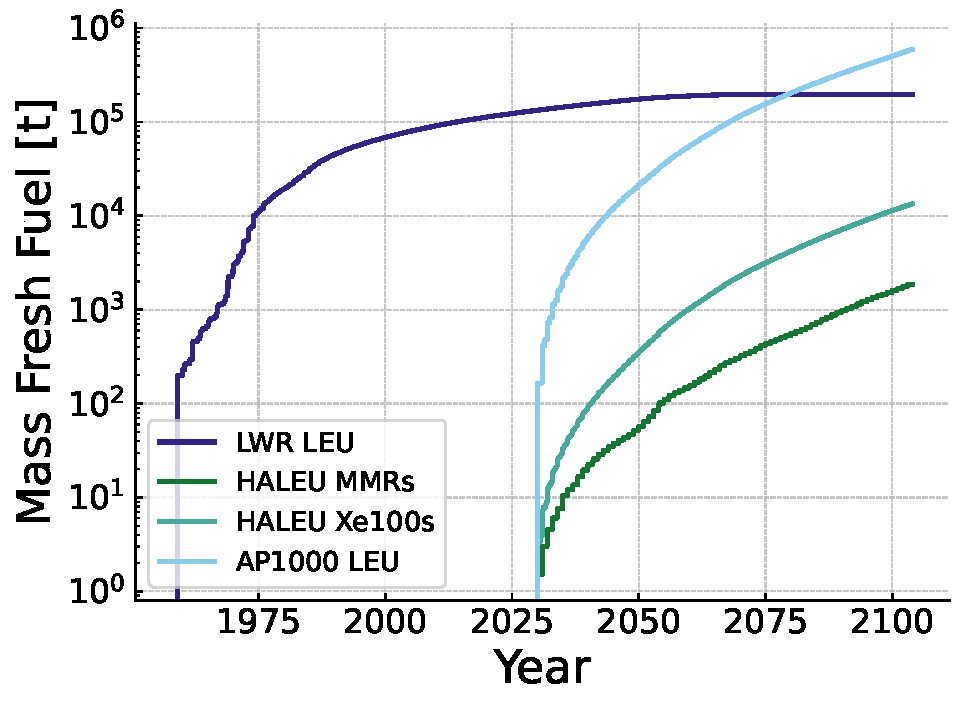
\includegraphics[width=0.495\textwidth]{images/results/fresh/one_dr2_fresh_fuel_cumulative_by_fuel.pdf}
   }
    \caption{Random single fresh fuel demanded.}
    \label{fig:random_of_fresh}
\end{figure}

In Table \ref{tab:random_fresh_avg} we show the average total yearly fresh fuel for the no growth and double scenarios in the single and multi fuel regimes under the random deployment scheme. The \gls{xe} reactors show a 796\% increase in the average total yearly fresh fuel going from the no growth scenario to the double scenario in the single fuel regime. The \gls{mmr} reactors show a 1505\% increase in the average total yearly fresh fuel going from the no growth scenario to the double scenario in the single fuel regime. The AP1000 reactors show a 696\% increase in the average total yearly fresh fuel going from the no growth scenario to the double scenario in the single fuel regime.

\begin{table}[H]
    \centering
    \caption{Average random yearly fresh fuel by design in tonnes.}
    \label{tab:random_fresh_avg}
    \begin{tabular}{c c c c c}
       \hline
       Scenario & No Growth, Single & No Growth, Multiple & Double, Single & Double, Multiple  \\
       \hline
       \gls{mmr} \gls{haleu}   & 0.128    & 0.128   & 2.055    & 2.033    \\
       \gls{mmr} \gls{leup}    & --       & --      & --       & 0.107    \\
       \gls{xe} \gls{haleu}    & 1.663    & 1.663   & 14.904   & 14.806   \\
       \gls{xe} \gls{leup}     & --       & --      & --       & 0.022    \\
       AP1000 \gls{leu}        & 82.512   & 82.512  & 656.698  & 656.698  \\
       \hline
    \end{tabular}
\end{table}





\subsection{Used Fuel Results}
\label{sec:random_used}

In Figures \ref{fig:random_mf_used} and \ref{fig:random_of_used} we can see the used fuel accumulation for the reactors in the no growth and double by 2050 scenarios. The used fuel curves in each scenario follow the reactor deployment curves with a lag corresponding to the cycle length of the reactor from Figures \ref{fig:random_mf_reactors} and \ref{fig:random_of_reactors}, as \cyclus removes fuel from each reactor.


% show total used fuel
\begin{figure}[H]
    \subfloat[No Growth \label{fig:random_mf_ng_used}]{%
      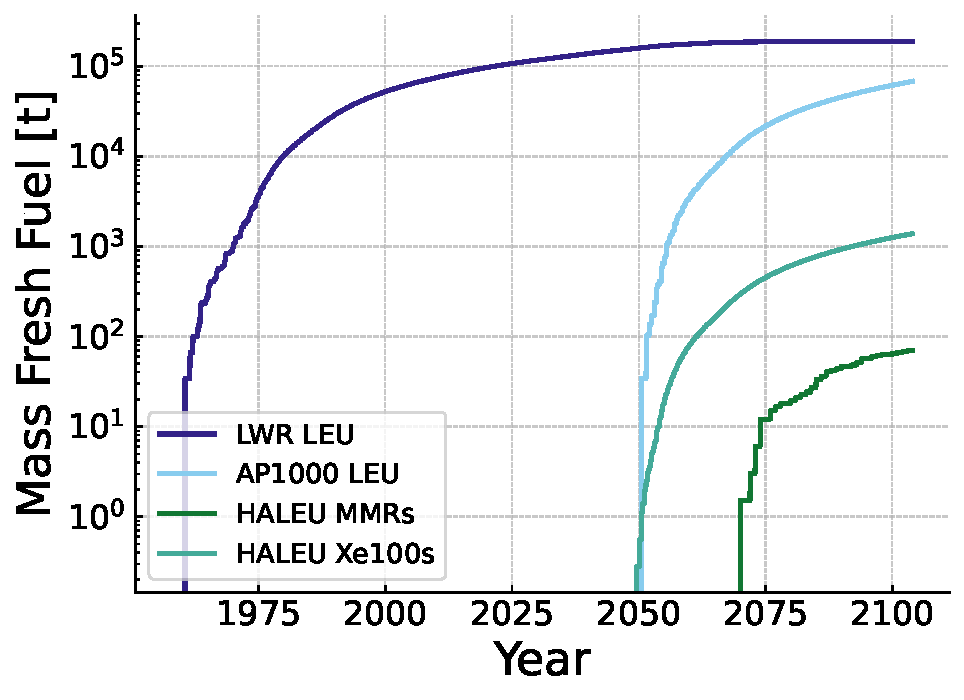
\includegraphics[width=0.495\textwidth]{images/results/used/multi_drng_used_fuel_cumulative_by_fuel.pdf}
   }
    \hfill
    \subfloat[Double \label{fig:random_mf_d2_used}]{%
      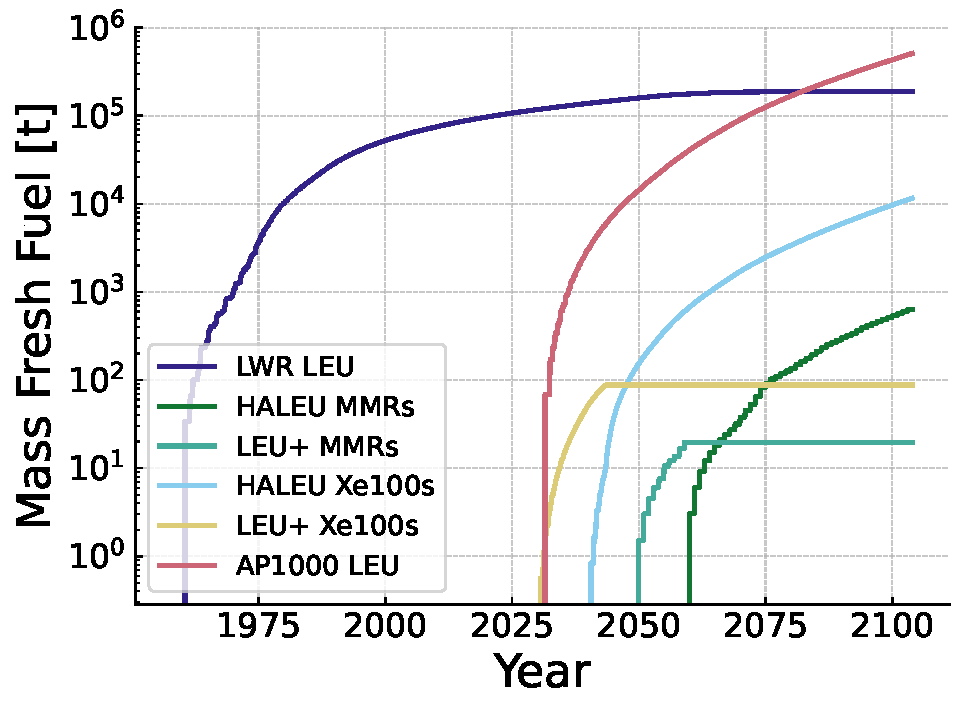
\includegraphics[width=0.495\textwidth]{images/results/used/multi_dr2_used_fuel_cumulative_by_fuel.pdf}
   }
    \caption{Random multi used fuel accumulation.}
    \label{fig:random_mf_used}
  \end{figure}


  \begin{figure}[H]
    \subfloat[No Growth \label{fig:random_of_ng_used}]{%
      \includegraphics[width=0.495\textwidth]{images/results/used/one_drng_used_fuel_cumulative_by_fuel.pdf}
   }
    \hfill
    \subfloat[Double \label{fig:random_of_d2_used}]{%
      \includegraphics[width=0.495\textwidth]{images/results/used/one_dr2_used_fuel_cumulative_by_fuel.pdf}
   }
    \caption{Random single used fuel accumulation.}
    \label{fig:random_of_used}
\end{figure}


In Table \ref{tab:random_used_avg} we show the average total yearly used fuel for the no growth and double scenarios in the single and multi fuel regimes under the random deployment scheme. The \gls{xe} reactors show a 742\% increase in the average total yearly used fuel going from the no growth scenario to the double scenario in the single fuel regime. The \gls{mmr} reactors show a 838\% increase in the average total yearly used fuel going from the no growth scenario to the double scenario in the single fuel regime. The AP1000 reactors show a 649\% increase in the average total yearly used fuel going from the no growth scenario to the double scenario in the single fuel regime.

\begin{table}[H]
    \centering
    \caption{Average random yearly used fuel by design in tonnes.}
    \label{tab:random_used_avg}
    \begin{tabular}{c c c c c}
       \hline
       Scenario & No Growth, Single & No Growth, Multiple & Double, Single & Double, Multiple  \\
       \hline
       \gls{mmr} \gls{haleu}   & 0.077    & 0.077   & 0.722    & 0.700    \\
       \gls{mmr} \gls{leup}    & --       & --      & --       & 0.107    \\
       \gls{xe} \gls{haleu}    & 1.536    & 1.536   & 12.930   & 12.833   \\
       \gls{xe} \gls{leup}     & --       & --      & --       & 0.022    \\
       AP1000 \gls{leu}        & 75.638   & 75.638  & 566.239  & 566.239  \\
       \hline
    \end{tabular}
\end{table}

% talk about repositories

\section{Initially Random, Greedy Deployment}
\label{sec:initially_random_greedy}

Combining the random and greedy deployment schemes allows us to inject uncertainty as to which reactor will be deployed at any given time while ensuring that the demand is met efficiently. This scheme does not give us more insight than the random or greedy deployment; it merely allows us to leverage the strengths of both.

This deployment scheme randomly deploys reactors until a reactor bigger than the remaining capacity is proposed for each year, then it fills the remaining capacity with a greedy algorithm. Figure \ref{fig:init_random_greedy_diagram} outlines, which shows the two loops (first random, then greedy) in the logic from the top down.

\begin{figure}[H]
  \centering
  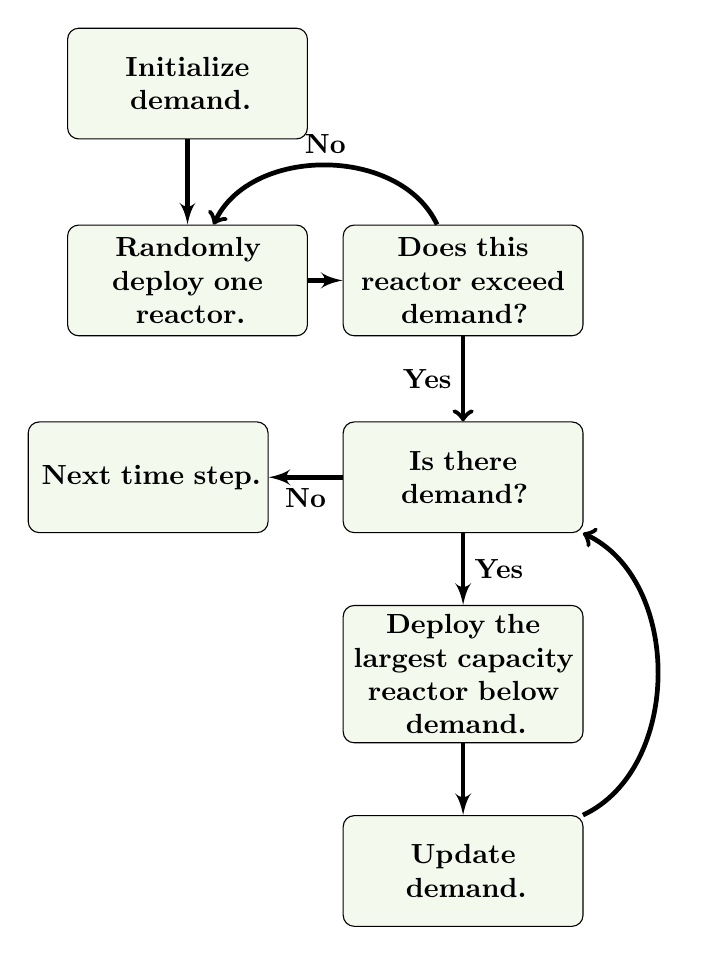
\begin{tikzpicture}[node distance = 2.5cm, auto]
    % Place random nodes
    \node [block] (init) {\textbf{Initialize demand.}};
    \node [block, below of=init, node distance=2.5cm] (evaluate) {\textbf{Randomly deploy one reactor.}};
    \node [block, right of=evaluate, node distance=3.5cm] (update) {\textbf{Does this reactor exceed demand?}};
    % Place greedy nodes
    \node [block, below of=update] (checkg) {\textbf{Is there demand?}};
    \node [block, below of=checkg, node distance=2.5cm] (evaluateg) {\textbf{Deploy the largest capacity reactor below demand.}};
    \node [block, below of=evaluateg, node distance=2.5cm] (updateg) {\textbf{Update demand.}};
    \node [block, left of=checkg, node distance=4cm] (stopg) {\textbf{Next time step.}};
    % Draw edges
    \path [line, line width=0.6mm] (init) -- (evaluate);
    \path [line, line width=0.6mm] (evaluate) -- (update);
    \draw[->, line width=0.6mm] (update) -- node[left]{\textbf{Yes}}(checkg);
    \draw[->, line width=0.6mm] (update) edge[bend right=65] node[above]{\textbf{No}} (evaluate);
    % Draw greedy edges
    \path [line, line width=0.6mm] (checkg) -- node {\textbf{Yes}} (evaluateg);
    \path [line, line width=0.6mm] (evaluateg) -- (updateg);
    \path [line, line width=0.6mm] (checkg) -- node {\textbf{No}}(stopg);
    \draw[->, line width=0.6mm] (updateg) edge[bend right=65] node[right]{} (checkg);
  \end{tikzpicture}
  \caption{The initially random, greedy deployment diagram demonstrates how the random and greedy deployment schemes complement each other for a single time step.}
  \label{fig:init_random_greedy_diagram}
\end{figure}

% \begin{figure}[H]
%     \centering
%     \includegraphics[scale=0.55]{images/schemes/random_greedy_diagram.png}
%     \caption{Initially random, greedy deployment diagram.}
%     \label{fig:init_random_greedy_diagram}
% \end{figure}

Section \ref{sec:random_deployment} highlights how this thesis did not implement the initially random, greedy deployment scheme to capture additional realism in the deployment problem. This scheme combines random and greedy deployment schemes and inherits their realistic and unrealistic elements. The random deployment scheme captures some of the complexity of the deployment problem but does not guarantee the capture of the nuance of future user needs. The greedy deployment scheme captures the efficiency of the deployment problem but does not capture the complexity of the deployment problem. This scheme is a compromise between the two and does not capture the nuance of the deployment problem.

The seed, which was set to 20240527121205 for every run for this scheme, for
the random number generator is set by the date and time of the simulation,
which allows for the reproducibility of the results. The degree to which this
scheme captures features of the random or greedy deployment schemes varies with
the number of reactors deployed in the random phase. Instead of randomly
deploying until the demand is met, this implementation randomly deploys until
the selected reactor exceeds the demand. This means that when the reactors are
different sizes, there is a chance that the random phase will deploy a reactor
larger than the demand, and the greedy phase will make up more of
the deployment.


\subsection{Number of Reactors}
\label{sec:rand_greed_reactors}

As with the random deployment scheme, Figures
\ref{fig:rand_greed_mf_reactors} and \ref{fig:rand_greed_of_reactors} show that the share of reactors by design is much closer than the greedy deployment scheme. The reactors in the \textit{no growth} scenarios (shown in Figures \ref{fig:rand_greed_mf_ng} and \ref{fig:rand_greed_of_ng}) are deployed close to 2050, whereas the advanced reactors in the \textit{double by 2050} scenarios (shown in Figures \ref{fig:rand_greed_mf_d2} and \ref{fig:rand_greed_of_d2}) are deployed close to 2030.

% Show total number of reactors multi-fuel
\begin{figure}[H]
    \subfloat[No Growth. \label{fig:rand_greed_mf_ng_reactors}]{%
      \includegraphics[width=0.495\textwidth]{images/results/reactors/multi_drgng_reactors.pdf}
   }
    \hfill
    \subfloat[Double. \label{fig:rand_greed_mf_d2_reactors}]{%
      \includegraphics[width=0.495\textwidth]{images/results/reactors/multi_drg2_reactors.pdf}
   }
    \caption{Multiple fuels initially random, then greedy reactor deployment.}
    \label{fig:rand_greed_mf_reactors}
  \end{figure}

% talk about the rate of deployment

% talk about the context of expanding energy needs

% talk about the workers

\begin{figure}[H]
    \subfloat[No Growth. \label{fig:rand_greed_of_ng_reactors}]{%
      \includegraphics[width=0.495\textwidth]{images/results/reactors/one_drgng_reactors.pdf}
   }
    \hfill
    \subfloat[Double. \label{fig:rand_greed_of_d2_reactors}]{%
      \includegraphics[width=0.495\textwidth]{images/results/reactors/one_drg2_reactors.pdf}
   }
    \caption{Single-fuel initially random, then greedy reactor deployment.}
    \label{fig:rand_greed_of_reactors}
\end{figure}

Table \ref{tab:rand_greed_reac_avg} shows the average total operating reactors by design for the \textit{no growth} and \textit{double by 2050} scenarios for the multi and single-fuel enrichment deployments. The \gls{haleu} fueled \gls{mmr} and \gls{xe} deployment is unchanged in the single and multi-fuel enrichment deployments for the \textit{no growth} scenarios. The number of AP1000 reactors increases 660\% from the \textit{no growth} to the \textit{double by 2050} scenario in the multi-fuel enrichment deployment. The number of \gls{haleu} fueled \gls{xe} reactors increases 626\%, while the number of \gls{haleu} fueled \gls{mmr} reactors increases 649\%.

\begin{table}[H]
    \centering
    \caption{Average initially random, then greedy total operating reactors by design.}
    \label{tab:rand_greed_reac_avg}
    \begin{tabular}{l c c c c}
       \toprule
       Scenario & \shortstack{No Growth,\\ Single} & \shortstack{No Growth,\\ Multiple} & \shortstack{Double,\\ Single} & \shortstack{Double,\\ Multiple}  \\
       \midrule
       \gls{haleu} fueled MMRs      & \textcolor{white}{0}44.547  & \textcolor{white}{0}44.547  & 333.613 & 325.347 \\
       \gls{leup} fueled MMRs       & --      & --      & --      & \textcolor{white}{00}8.267   \\
       \gls{haleu} fueled \gls{xe}s & \textcolor{white}{0}47.52   & \textcolor{white}{0}47.52   & 344.88  & 317.68  \\
       \gls{leup} fueled \gls{xe}s  & --      & --      & --      & \textcolor{white}{0}27.2    \\
       \gls{leu} fueled AP1000      & \textcolor{white}{0}42.72   & \textcolor{white}{0}42.72   & 324.68  & 324.68  \\
       \bottomrule
    \end{tabular}
\end{table}

\subsection{SWU Results}
\label{sec:rand_greed_swu}

Figure \ref{fig:swu_yearly_rand_greed} shows the yearly \gls{swu} demand periodically spike as reactors begin operation in the depicted \textit{no growth} scenario around 2050. The \gls{swu} demand for the AP1000 \gls{leu} rises above the other two reactors while the demand from \glspl{xe} overlaps heavily with the demand from \glspl{mmr}. This trend is exacerbated in the \textit{double by 2050} scenarios shown in Figures \ref{fig:rand_greed_mf_d2_swu} and \ref{fig:rand_greed_of_d2_swu} where the \gls{swu} for AP1000 \gls{leu} fuel rises quickly and eventually exceeds the total \gls{swu} for the existing fleet.
% talk about the SWU capacity

% show the total SWU capacity
\begin{figure}[H]
    \centering
    \includegraphics[scale=0.7]{images/results/swu/multi_drgng_swu_by_fuel.pdf}
    \caption{Initially random, then greedy yearly SWU demand.}
    \label{fig:swu_yearly_rand_greed}
\end{figure}

As the features of the yearly data are regular, dictated by the cycles of the reactors, and overlapping, Figures \ref{fig:rand_greed_mf_swu} and \ref{fig:rand_greed_of_swu} visualize the total cumulative \gls{swu} demand.


\begin{figure}[H]
  \subfloat[No Growth. \label{fig:rand_greed_mf_ng_swu}]{%
    \includegraphics[width=0.495\textwidth]{images/results/swu/multi_drgng_swu_cumulative_by_fuel.pdf}
 }
  \hfill
  \subfloat[Double. \label{fig:rand_greed_mf_d2_swu}]{%
    \includegraphics[width=0.495\textwidth]{images/results/swu/multi_drg2_swu_cumulative_by_fuel.pdf}
 }
  \caption{Initially random, then greedy multi-fuel SWU.}
  \label{fig:rand_greed_mf_swu}
\end{figure}



\begin{figure}[H]
    \subfloat[No Growth. \label{fig:rand_greed_of_ng_swu}]{%
      \includegraphics[width=0.495\textwidth]{images/results/swu/one_drgng_swu_cumulative_by_fuel.pdf}
   }
    \hfill
    \subfloat[Double. \label{fig:rand_greed_of_d2_swu}]{%
      \includegraphics[width=0.495\textwidth]{images/results/swu/one_drg2_swu_cumulative_by_fuel.pdf}
   }
    \caption{Initially random, then greedy single-fuel SWU.}
    \label{fig:rand_greed_of_swu}
\end{figure}

% talk about international trade

Table \ref{tab:rand_greed_swu_avg} shows the average yearly \gls{swu} for the \textit{no growth} and \textit{double by 2050} scenarios for the multi and single-fuel enrichment deployments. The \gls{swu} demand for the \gls{mmr} and \gls{xe} reactors is the same in the single and multi-fuel enrichment deployments for the \textit{no growth} scenarios, which is consistent with the reactor deployment trends in the Section \ref{sec:rand_greed_reactors}. Across scenarios, the demand for \gls{swu} for AP1000 \gls{leu} fuel increases 696\% from the \textit{no growth} to the \textit{double by 2050} scenario in the single-fuel enrichment deployment. The demand for \gls{swu} for \gls{haleu} fuel in the \gls{mmr} and \gls{xe} reactors increases 775\% and 672\% respectively from the \textit{no growth} to the \textit{double by 2050} scenario in the multi-fuel enrichment deployment.

\begin{table}[H]
    \centering
    \caption{Average initially random, then greedy yearly SWU by design in k\gls{swu}.}
    \label{tab:rand_greed_swu_avg}
    \begin{tabular}{l c c c c}
       \toprule
       Scenario & \shortstack{No Growth,\\ Single} & \shortstack{No Growth,\\ Multiple} & \shortstack{Double,\\ Single} & \shortstack{Double,\\ Multiple}  \\
       \midrule
       \gls{mmr} \gls{haleu}   & \textcolor{white}{00}16.738  & \textcolor{white}{00}16.738  & \textcolor{white}{0}146.477  & \textcolor{white}{0}144.129  \\
       \gls{mmr} \gls{leup}    & --      & --      & --       & \textcolor{white}{000}1.079    \\
       \gls{xe} \gls{haleu}    & \textcolor{white}{00}70.066  & \textcolor{white}{00}70.066  & \textcolor{white}{0}540.613  & \textcolor{white}{0}534.559  \\
       \gls{xe} \gls{leup}     & --      & --      & --       & \textcolor{white}{000}3.624    \\
       AP1000 \gls{leu}        & \textcolor{white}{0}634.553 & \textcolor{white}{0}634.553 & 5050.323 & 5050.323 \\
       \bottomrule
    \end{tabular}
\end{table}



\subsection{Fresh Fuel Results}
\label{sec:rand_greed_fresh}

% talk about the types of fuel
Figures \ref{fig:rand_greed_mf_fresh} and \ref{fig:rand_greed_of_fresh} show the fresh fuel demand for the reactors in the \textit{no growth} and \textit{double by 2050} scenarios. The fresh fuel curves in each scenario follow the same pattern as the reactor deployment curves from Figures \ref{fig:rand_greed_mf_reactors} and \ref{fig:rand_greed_of_reactors}, as \cyclus supplies fuel to each of the reactors as it they deploy.


% show total fresh fuel
\begin{figure}[H]
    \subfloat[No Growth. \label{fig:rand_greed_mf_ng_fresh}]{%
      \includegraphics[width=0.495\textwidth]{images/results/fresh/multi_drgng_fresh_fuel_cumulative_by_fuel.pdf}
   }
    \hfill
    \subfloat[Double. \label{fig:rand_greed_mf_d2_fresh}]{%
      \includegraphics[width=0.495\textwidth]{images/results/fresh/multi_drg2_fresh_fuel_cumulative_by_fuel.pdf}
   }
    \caption{Initially random, then greedy multi fresh fuel demanded.}
    \label{fig:rand_greed_mf_fresh}
  \end{figure}

% talk about transportation of fuel


\begin{figure}[H]
    \subfloat[No Growth. \label{fig:rand_greed_of_ng_fresh}]{%
      \includegraphics[width=0.495\textwidth]{images/results/fresh/one_drgng_fresh_fuel_cumulative_by_fuel.pdf}
   }
    \hfill
    \subfloat[Double. \label{fig:rand_greed_of_d2_fresh}]{%
      \includegraphics[width=0.495\textwidth]{images/results/fresh/one_drg2_fresh_fuel_cumulative_by_fuel.pdf}
   }
    \caption{Initially random, then greedy single fresh fuel demanded.}
    \label{fig:rand_greed_of_fresh}
  \end{figure}

Table \ref{tab:rand_greed_fresh_avg} shows the average yearly fresh fuel by design in tonnes for the \textit{no growth} and \textit{double by 2050} scenarios for the multi and single-fuel enrichment deployments. The fresh fuel demand for the reactors is the same in the single and multi-fuel enrichment deployments for the \textit{no growth} scenarios, which is consistent with the reactor deployment trends in the Section \ref{sec:rand_greed_reactors}. Across scenarios, the demand for fresh fuel for AP1000 \gls{leu} fuel increases 696\% from the \textit{no growth} to the \textit{double by 2050} scenario in the single-fuel enrichment deployment. The demand for fresh fuel for \gls{haleu} fuel in the \gls{mmr} and \gls{xe} reactors increases 775\% and 671\% respectively from the \textit{no growth} to the \textit{double by 2050} scenario in the multi-fuel enrichment deployment.

\begin{table}[H]
    \centering
    \caption{Average initially random, then greedy yearly fresh fuel by design in tonnes.}
    \label{tab:rand_greed_fresh_avg}
    \begin{tabular}{l c c c c}
       \toprule
       Scenario & \shortstack{No Growth,\\ Single} & \shortstack{No Growth,\\ Multiple} & \shortstack{Double,\\ Single} & \shortstack{Double,\\ Multiple}  \\
       \midrule
       \gls{mmr} \gls{haleu}   & \textcolor{white}{00}0.371    & \textcolor{white}{00}0.371   & \textcolor{white}{00}3.247    & \textcolor{white}{00}3.194    \\
       \gls{mmr} \gls{leup}    & --       & --      & --       & \textcolor{white}{00}0.052    \\
       \gls{xe} \gls{haleu}    & \textcolor{white}{00}2.033    & \textcolor{white}{00}2.033   & \textcolor{white}{0}15.683   & \textcolor{white}{0}15.507   \\
       \gls{xe} \gls{leup}     & --       & --      & --       & \textcolor{white}{00}0.176    \\
       AP1000 \gls{leu}        & \textcolor{white}{0}82.512   & \textcolor{white}{0}82.512  & 656.698  & 656.698  \\
       \bottomrule
    \end{tabular}
\end{table}


\subsection{Used Fuel Results}
\label{sec:rand_greed_used}

Figures \ref{fig:rand_greed_mf_used} and \ref{fig:rand_greed_of_used} depict the used fuel accumulation for the reactors in the \textit{no growth} and \textit{double by 2050} scenarios. The used fuel curves in each scenario follow the reactor deployment curves with a lag corresponding to the cycle length of the reactor from Figures \ref{fig:rand_greed_mf_reactors} and \ref{fig:rand_greed_of_reactors}, as \cyclus removes fuel from each reactor.


% show total used fuel
\begin{figure}[H]
    \subfloat[No Growth. \label{fig:rand_greed_mf_ng_used}]{%
      \includegraphics[width=0.495\textwidth]{images/results/used/multi_drgng_used_fuel_cumulative_by_fuel.pdf}
   }
    \hfill
    \subfloat[Double. \label{fig:rand_greed_mf_d2_used}]{%
      \includegraphics[width=0.495\textwidth]{images/results/used/multi_drg2_used_fuel_cumulative_by_fuel.pdf}
   }
    \caption{Initially random, then greedy multi used fuel accumulation.}
    \label{fig:rand_greed_mf_used}
  \end{figure}


  \begin{figure}[H]
    \subfloat[No Growth. \label{fig:rand_greed_of_ng_used}]{%
      \includegraphics[width=0.495\textwidth]{images/results/used/one_drgng_used_fuel_cumulative_by_fuel.pdf}
   }
    \hfill
    \subfloat[Double. \label{fig:rand_greed_of_d2_used}]{%
      \includegraphics[width=0.495\textwidth]{images/results/used/one_drg2_used_fuel_cumulative_by_fuel.pdf}
   }
    \caption{Initially random, then greedy single used fuel accumulation.}
    \label{fig:rand_greed_of_used}
  \end{figure}


Table \ref{tab:rand_greed_used_avg} shows the average yearly used fuel by design in tonnes for the \textit{no growth} and \textit{double by 2050} scenarios for the multi and single-fuel enrichment deployments. The used fuel demand for the reactors is the same in the single and multi-fuel enrichment deployments for the \textit{no growth} scenarios, which is consistent with the reactor deployment trends in the Section \ref{sec:rand_greed_reactors}. Across scenarios, the demand for used fuel for AP1000 \gls{leu} fuel increases 649\% from the \textit{no growth} to the \textit{double by 2050} scenario in the single-fuel enrichment deployment. The demand for used fuel for \gls{haleu} fuel in the \gls{mmr} and \gls{xe} reactors increases 503\% and 620\% respectively from the \textit{no growth} to the \textit{double by 2050} scenario in the multi-fuel enrichment deployment.

  \begin{table}[H]
    \centering
    \caption{Average initially random, then greedy yearly used fuel by design in tonnes.}
    \label{tab:rand_greed_used_avg}
    \begin{tabular}{l c c c c}
       \toprule
       Scenario & \shortstack{No Growth,\\ Single} & \shortstack{No Growth,\\ Multiple} & \shortstack{Double,\\ Single} & \shortstack{Double,\\ Multiple}  \\
       \midrule
       \gls{mmr} \gls{haleu}   & \textcolor{white}{00}0.185    & \textcolor{white}{00}0.185   & \textcolor{white}{00}1.115    & \textcolor{white}{00}1.063    \\
       \gls{mmr} \gls{leup}    & --       & --      & --       & \textcolor{white}{00}0.052    \\
       \gls{xe} \gls{haleu}    & \textcolor{white}{00}1.882    & \textcolor{white}{00}1.882   & \textcolor{white}{0}13.549   & \textcolor{white}{0}13.419   \\
       \gls{xe} \gls{leup}     & --       & --      & --       & \textcolor{white}{00}0.176    \\
       AP1000 \gls{leu}        & \textcolor{white}{0}75.638   & \textcolor{white}{0}75.638  & 566.239  & 566.239  \\
       \bottomrule
    \end{tabular}
  \end{table}

% talk about repositories


\chapter{Reactor Power and Market Interactions}
\label{ch:time}
\glsresetall

This chapter explores how altering the frequency with which the \cycamore reactor interacts with the \gls{dre} in \cyclus impacts the computational efficiency of a simulation and how to make the power output from a reactor more realistic.

\section{Archetypes and Time Management}
\label{sec:archetypes_and_time_management}

Throughout the \cyclus ecosystem, archetypes interact with the \gls{dre} and
each other in a fixed, user-defined time step, forcing the entire simulation
to operate on the smallest universal time step. For example, if a fabrication
facility can produce material every 2 months but the enrichment facility can
only provide material every 3 months, \cyclus would need to use a 1-month time step to capture both. When the time step is smaller than the minimum for a given
facility, that facility still participates in the \gls{dre} with a zero bid.
These zero bids, across hundreds of facilities, add complexity and
inefficiencies to solving the transaction problem at each time step.

In the \cyclus ecosystem there is an archetype called \textit{PatternSink} wherein the user can alter the frequency at which the sink, often called the repository, can accept the material. Figure \ref{fig:a-b-c} outlines an example scenario for this archetype with a simple A-B-C flow path. In this scenario, material is received from a source (A) to a reactor (B) with a final (C) sink that can only accept material at a specific frequency.

\begin{figure}[H]
    \centering
    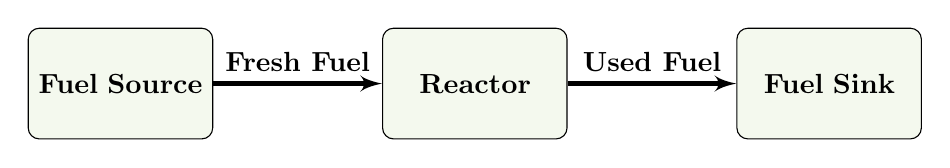
\begin{tikzpicture}
        % Place nodes
        \node [abc] (reactor) {\textbf{Reactor}};
        \node [abc, left of=reactor, node distance=4.5cm] (source) {\textbf{Fuel Source}};
        \node [abc, right of=reactor, node distance=4.5cm] (sink) {\textbf{Fuel Sink}};
        % Draw edges
        \path [line, line width=0.6mm] (source) -- node[above]{\textbf{Fresh Fuel}} (reactor);
        \path [line, line width=0.6mm] (reactor) -- node[above]{\textbf{Used Fuel}} (sink);
    \end{tikzpicture}
    \caption{Simple A-B-C scenario.}
    \label{fig:a-b-c}
\end{figure}

% \begin{figure}[H]
%     \centering
%     \includegraphics[scale=0.4]{images/cyclus/a-b-c.png}
%     \caption{Simple A-B-C scenario.}
%     \label{fig:a-b-c}
% \end{figure}

Examining the material that the sink receives, it becomes clear that this
frequency alters how frequently the archetype updates its internal
understanding of time. It appears in Figure \ref{fig:pattern_freq_50} as though
multiple groups of material are received in one time step despite this
archetype not having an idea of individual shipments. This archetype
accomplishes the artificial restriction on accepting material by simply not
updating the time step that the archetype is at until the next universal time
step is met. Regardless of function, this is the only example of the
timekeeping flexibility found in the ecosystem.

\begin{figure}[H]
    \centering
    \includegraphics[scale=0.7]{images/cyclus/pattern_sink_fuel_transactions.pdf}
    \caption{Acceptance of $^{239}$Pu into the Sink with a frequency of 50 months.}
    \label{fig:pattern_freq_50}
\end{figure}

While archetypes like \textit{PatternSink} introduce new internal capabilities, they all inherit a set of base capabilities from the \cyclus toolkit. The \cyclus toolkit provides a modular and extensible framework for modeling \glspl{nfc}, allowing users to create custom archetypes that simulate various facilities and processes. These base capabilities standardize how archetypes create material buffers, interact with the \gls{dre}, and connect to the internal clock of the simulation, which are essential for coordinating the agents and commodities across their complex interactions within an \gls{nfc}. This thesis examines the fundamental capabilities of the \cyclus ecosystem and identifies time-intensive components of the current \cycamore Reactor. Section \ref{sec:trading_reactor} of this thesis creates an archetype called the \gls{tod} reactor, that interacts with the \gls{dre} only when it is time to refuel.

The toolkit’s modular architecture allows users to integrate new archetypes and models, promoting innovation and collaboration within the \cyclus community. This thesis contributes a reactor archetype called \gls{dpr} to the ecosystem that can adjust the power of the reactor based on user inputs to better capture real fluctuations in reactor operation. Through this archetype, this thesis explores incorporating historical realism and allowing for small timescale simulations to better capture the power output dynamics of the reactor fleet.

\section{Trading On-Demand Reactor}
\label{sec:trading_reactor}
% Review the literature related to the third subtopic. Summarize key findings and highlight important studies.

% Start with Cyclus time, go into pattern sink, and then archetype time toolkit update.
As Section \ref{sec:archetypes_and_time_management} discusses, \cyclus simulations have a universal time step at which every facility operates. The \cycamore reactor, like other archetypes, operates on this universal time step and interacts with the \gls{dre} at every time step. This interaction is necessary for the reactor to receive fuel and to bid on material from other facilities. However, this interaction is not necessary if the reactor does not need to refuel.

% Normal reactor
% 5,202,746,245 (52.57%)  => /home/rhysmac/cyclus/src/exchange_manager.h:cyclus::ExchangeManager<cyclus::Material>::Execute() (24x)
% 1,312,800,228 (13.26%)  => ???:cycamore::Reactor::Tock() (18,000x)
% 461,172,309 ( 4.66%)  => ???:cycamore::Reactor::Tick() (18,000x)
Valgrind's \cite{valgrind} Callgrind \cite{callgrind} tool profiles a source-reactor-sink scenario and establish which parts of the \cycamore reactor code generate the most instructions. 52.27\% of the 9,897,385,005 instructions come from the exchange manager in \cyclus, and the reactor's tock (which appends each time step) is the source of 13.26\% of the instructions. The reactor's tick (which pre-pends each time step) is the source of 4.66\% of the instructions.

The basic structure of each time step is fundamental to aligning the material transactions and bids in the existing \gls{dre}, so a reduction in computational cost could come from checking whether or not it is time to refuel before engaging with the calculations that take place when the reactor needs to refuel. This new archetype is called the \gls{tod} reactor, and the tock was the source of 11.5\% of the 9,519,845,814 instructions, while tick was the source of 2.77\% of the instructions.

% Silent reactor
% 5,083,560,026 (53.40%)  => /home/rhysmac/cyclus/src/exchange_manager.h:cyclus::ExchangeManager<cyclus::Material>::Execute() (24x)
% 1,094,637,634 (11.50%)  => ???:cycamore::SilentReactor::Tock() (18,102x)
% 264,086,388 ( 2.77%)  => ???:cycamore::SilentReactor::Tick() (18,102x)


There are ten duplicates in this thesis of a simple source-reactor-sink scenario to further compare how the \cycamore and \gls{tod} reactors perform and collected statistics with the Linux tool Perf \cite{perf}. In these scenarios, \cyclus deploys 1000 reactors over the first ten time steps, and the reactors operate for three time steps before refueling for two. This scenario demonstrates an intensive deployment to exacerbate the differences between the two reactor archetypes. The mean, maximum, minimum, and standard deviation of the wall clock time, number of instructions, and instructions per cycle are in Table \ref{tab:tod_profile}.

% make a table for the time_context max, min, average, and standard deviation
\begin{table}[H]
    \centering
    \caption{\gls{tod} reactor and \cycamore reactor fleet simulation profiles showing the max, min, mean, and standard deviation of the wall time, number of instructions, and instructions per cycle.}
    \label{tab:tod_profile}
    \begin{tabular}{l l l l l l}
        \hline
        Reactor & Metric & Mean & Max & Min & StDev\\
        \hline
        \cycamore Reactor & wall clock time [sec] & 3.286 & 3.333 & 3.242 & 0.026\\
         & Instructions & $1.209 \times10^{10}$ & $1.211 \times10^{10}$ & $1.207 \times10^{10}$ & $1.328 \times10^{7}$\\
         & Instructions per Cycle & 0.800 & 0.808 & 0.791 & 0.005\\
        \gls{tod} Reactor & wall clock time [sec] & 3.166 & 3.195 & 3.142 & 0.016 \\
        & Instructions & $1.174 \times10^{10}$ & $1.176 \times10^{10}$ & $1.167 \times10^{10}$ & $2.692 \times10^{7}$\\
         & Instructions per Cycle & 0.807 & 0.811 & 0.801 & 0.003\\
        \hline
    \end{tabular}
\end{table}

The results in Table \ref{tab:tod_profile} indicate an average speedup of 1.038, going from the \cycamore reactor to the \gls{tod} reactor. As Figure \ref{fig:time_violin} indicates, these time results are significant outside their combined standard deviations.

\begin{figure}[H]
    \centering
    \includegraphics[width=0.7\linewidth]{images/power_reactor/time_clock_violin.pdf}
    \caption{Wall clock time values for the \gls{tod} and \cycamore reactors.}
    \label{fig:time_violin}
\end{figure}

The wall clock time values can vary by machine, architecture, and other demands during operation; however, the number of instructions issued using these archetypes, shown in Figure \ref{fig:isn_violin}, is distinct between the \gls{tod} and \cycamore reactors and is specific to the code, not the machine. The distributions of instructions per cycle, presented alongside the instructions, overlap but indicate that the average \gls{tod} reactor simulation has a higher utilization than the \cycamore reactor.

\begin{figure}[H]
    \subfloat[Number of instructions for \gls{tod} and the \cycamore Reactor.\label{fig:ins_tod_cyc}]{%
      \includegraphics[width=0.49\textwidth]{images/power_reactor/ins_violin.pdf}
   }
    \hfill
    \subfloat[Number of instructions per cycle for \gls{tod} and the \cycamore Reactor.\label{fig:ins_per_cyc}]{%
      \includegraphics[width=0.49\textwidth]{images/power_reactor/ins_per_cyc.pdf}
   }
    \caption{Comparing the number of instructions and instructions per cycle for the \gls{tod} and \cycamore reactors shows that \gls{tod} has a higher utilization.}
    \label{fig:isn_violin}
\end{figure}

\section{Dynamic Power Reactor}
\label{sec:dpr_method}

The \gls{nrc} publishes a daily Power Reactor Status report for each reactor
under its jurisdiction \cite{nrc_power_2025}. These reports contain, amongst
other things, the percentage of the total power at which the operators
say the reactor operated. In the case of a fuel cycle simulation containing a
small number of reactors or a full-fleet simulation over a short time, the
differences in the power predicted by the \cycamore reactor and reality can
diverge.

Figure \ref{fig:pp_full} examines the single reactor operating at the
\gls{clinton}, with a reference unit power (i.e., net power) of 1062
MWe according to the \gls{iaea} \gls{pris} database \cite{IAEA_PRIS}, and
compare it to the results from the \cycamore reactor modeled over the same time
frame. This figure excludes the startup of the \cycamore reactor to ensure that it was operating on the same schedule as the data from the \gls{nrc} suggest the reactor was operating on from the start of 2021 through the end of 2024.

\begin{figure}[H]
  \centering
  \includegraphics[width=0.7\linewidth]{images/power_reactor/power_percent_clinton_fake.pdf}
  \caption{\gls{clinton} reactor daily capacity factor 2021-2024.}
  \label{fig:pp_full}
\end{figure}

A simple numerical integration reveals that the total energy capacity of both reactors differs by just under 51 GWe with a percent difference of 3.52\%. This difference can be negated by comparing it to a base case, but for the small-scale model, users might be interested in incorporating realistic fluctuations in power and find that the two scenarios in Figure \ref{fig:pp_full} were not equal on 908 days, or 62.2\%, of the 1460-day simulation. This thesis introduces the \gls{dpr} to mirror this variability in power of an operating reactor, as shown in Figure \ref{fig:pp_full}. \gls{dpr} functions the same way as the \cycamore reactor, except the user can input the percentage of the total capacity the reactor is outputting at any given time step.


\begin{figure}[H]
  \centering
  \includegraphics[width=0.7\linewidth]{images/power_reactor/dpr_diff.pdf}
  \caption{Difference in daily capacity factor between \gls{dpr} and \gls{clinton}.}
  \label{fig:dpr_clinton_diff}
\end{figure}


Narrowing the scope of this study to 2024, Figure \ref{fig:dpr_clinton_diff} shows how \gls{dpr} replicates capacity factor fluctuations with the difference between the reported values from the \gls{nrc} \cite{nrc_power_2025} and the results from the \cyclus simulation. The maximum difference between the two is $2.22 \times 10^{-16}$, which is explainable by floating point error in calculations as this value matches a double point machine epsilon value. Figure \ref{fig:dpr_cycamore_power} compares \gls{dpr} to the \cycamore reactor. As the reactors are assumed to start operations before 2024, a buffer month in which the reactors receive fuel allows these results to align with reality. The vertical line indicates when 2024 begins, allowing Figure \ref{fig:dpr_cycamore_power} to compare the \gls{nrc} data with results from \cyclus.


\begin{figure}[H]
  \centering
  \includegraphics[width=0.7\linewidth]{images/power_reactor/dpr_cycamore_energy.pdf}
  \caption{2024 capacity factor of the \cycamore reactor and \gls{dpr}.}
  \label{fig:dpr_cycamore_power}
\end{figure}




\chapter{Conclusions}
\label{ch:conclusions}
\glsresetall

\section{Transition Scenarios Conclusions}
\label{sec:dep_conc}

% 1. What are the SWU requirements for TRISO fueled reactor transitions that incorporate the proposed LEU+ to HALEU scheme?
% 2. If we have x growth of demand met by ARs, how much TRISO do we need, and when do we meet the demand?
% 3. What are the impacts of deployment schemes in NFC scenarios, and what parts are realistic or unrealistic in each? How quickly/often does the scenario meet the energy demand (we would need to identify limiting factors)?

In this work, we have characterized and contextualized bounding scenarios of reactor deployment in the \gls{usa} as we transition to a new fleet of nuclear reactors using an interstitial fuel cycle involving \gls{leup} \gls{triso} fuel. The results of this work show that the reactor deployment scheme has an understandable and identifiable impact on the \gls{swu} required to meet the energy demand.

In the transition scenarios of this work, we propose a series of fuel cycles that include and contextualize the deployment of new nuclear reactors in the \gls{usa} using \gls{triso} fuels at \gls{haleu} and \gls{leup} enrichment levels. These fuel cycles meet the energy demand growths predicted by the \gls{eia} and \gls{doe}. The increase in demand assumes that nuclear energy's generation share remains constant over time. When we say a 15$\%$ increase in demand, we mean a 15$\%$ increase in nuclear energy generation (as the EIA numbers \cite{eia_aeo_2023} reflect the total energy demand, this conversion is only possible by assuming that the percentage share of nuclear capacity is the same). This assumption is not reflected in the demand scenarios from the \gls{doe} liftoff report \cite{julie_liftoff_pathways_2024}, which are specific to nuclear deployment increases, and the number is agnostic to the total increase. The liftoff report scenarios are assumed to continue beyond the initial 2050 projection.

The \gls{lwr} fleet deviates from reality as we assume they all have regular 18-month cycles with regular 1-month outages. Related to this consistent cycle length, we assume that the reactors have constant power outputs (when not in an outage) over their lifetime. Each \gls{lwr} has an assembly size of 427.38589211618256 and a batch size of 80,  further normalizing the fleet. After 2024, no new \gls{lwr} are built other than the AP1000s deployed under the various schemes.

We assume that the supply chain is not a limiting factor in new reactors. This allows us to characterize the upper bound of what needs to be in place to achieve the projected deployment scenarios. Additionally, we treat the fabrication and enrichment of fuel as a black box, not factoring in variations in time, resources, or regulations associated with the fuels included.

We based the models used for the \gls{mmr} and \gls{xe} Serpent simulations on limited publicly available information and do not rely on confidential or proprietary data, and another limitation is they assume that when the reactors accept \gls{leup} fuel and operate with the same power levels and burnup rates. As we have discussed, the intended use of many advanced reactors extends beyond simply meeting energy demand, so modeling them entirely in on-the-grid applications is not necessarily the only way they will deploy. These reactors could provide a range of services that can contribute to decarbonizing the economy.

The result of these assumptions is that we expect the changes in \gls{swu} to be the most significant metric to compare the scenarios. In Table \ref{tab:swu_incs}, we show the average yearly percentage \gls{swu} increases from the no-growth scenario to the double scenario. We can see the impacts of the deployment scheme in these values, where the greedy scheme regularly prefers the highest capacity reactors, leading to the most significant increase in the \gls{swu} for AP1000 \gls{leu}. The randomness in the other two schemes levels the reactor preferences and leads to more consistent increases across fuel types.

\begin{table}[H]
    \centering
    \caption{Average yearly percentage \gls{swu} increases from the no-growth scenario to the double scenario.}
    \label{tab:swu_incs}
    \begin{tabular}{c c c c}
        \hline
        Scheme & \gls{mmr} \gls{haleu} & \gls{xe} \gls{haleu} & AP1000 \gls{leu}\\
        \hline
        Greedy Deployment & 105\% & 167\% & 800\% \\
        Random Deployment & 1511\% & 796\% & 697\% \\
        Initially Random Greedy & 775\% & 672\% & 696\% \\
        \hline
    \end{tabular}
\end{table}

% The mass of fresh fuel required to deploy the reactors as proposed in this work is staggering. As shown in Table \ref{tab:fresh_incs}, the percentage increase of average fresh fuel mass from the no-growth scenario to the double scenario mirrors the values from Table \ref{tab:swu_incs}.

% \begin{table}[H]
%     \centering
%     \caption{Average yearly percentage fresh fuel increases from the no-growth scenario to the double scenario.}
%     \label{tab:fresh_incs}
%     \begin{tabular}{c c c c}
%         \hline
%         Scheme & \gls{mmr} \gls{haleu} & \gls{xe} \gls{haleu} & AP1000 \gls{leu}\\
%         \hline
%         Greedy Deployment & 105\% & 159\% & 800\% \\
%         Random Deployment & 1505\% & 796\% & 696\% \\
%         Initially Random Greedy & 775\% & 671\% & 696\% \\
%         \hline
%     \end{tabular}
% \end{table}



\subsection{Future Work}
\label{sec:future_work}

This work could be expanded in a variety of ways to better contextualize the deployment of advanced reactors in the \gls{usa}. Outside of simply removing the assumptions outlined above, two immediate additions to this work would be to incorporate isotope calculations for the used fuel in this work to better understand the accumulation of isotopes of interest. This would allow for a more detailed understanding of the waste stream and the potential for recycling. The second addition would be to compare the no growth and double nuclear scenarios to the triple nuclear scenario from the \gls{doe} liftoff report \cite{julie_liftoff_pathways_2024}. These two additions were not included in this work due to computational limitations and the sheer size of the data needed, despite both being set up.

The next steps for expanding this work would be to translate the base metrics presented here (\gls{swu}, mass, energy, and deployment) into costs for fuel and energy. The mass of used fuel would be a good starting point for repository space considerations, and transportation costs. This work could take advantage of \cyclus's ability to track latitude and longitude to better understand the time of transportation between facilities.

As we highlighted in our discussion of \gls{leup}, the categories of enrichment facility are critical components in the cost and logistics of a fuel cycle. \gls{swu} is a good starting point for understanding the relative effort required to deploy the reactors, but the cost of that effort is a critical component of the deployment for making policy recommendations. Combining \gls{swu} and masses of fuel, we can start to understand how international cooperation with nations that have existing enrichment facilities could help the \gls{usa} meet its energy goals.

% assumptions
% \begin{itemize}
    % \item The demand increase assumes that nuclear energy's share of generation remains constant over time. When we say a 15$\%$ increase in demand, we mean a 15$\%$ increase in nuclear energy generation (as the EIA numbers \cite{eia_aeo_2023} are meant to reflect the total energy demand, this conversion is only possible by assuming that the percentage share of nuclear capacity is the same). This assumption is not reflected in the demand scenarios from the \gls{doe} liftoff report \cite{julie_liftoff_pathways_2024}, which are specific to nuclear deployment increases and the number is agnostic to the total increase. The liftoff report scenarios are assumed to continue beyond the initial 2050 projection.
    % \item \gls{lwr}s have an 18 month cycle with no deviation.
    % \item \gls{lwr}s have a regular 1 month outage.
    % \item \gls{lwr}s have an assembly size of 427.38589211618256.
    % \item \gls{lwr}s have a batch size of 80.
    % \item All reactors have constant power output (when not in outage) over their lifetime.
    % \item No new \gls{lwr}s are built after 2024. % not really the case anymore
    % \item \gls{lwr}s have no additional outages other than the regular 1 month outage.
    % \item Essentially assume that the supply chain is not a limiting factor in the deployment of new reactors, we make no requirements that it is necessarily located in the \gls{usa}, but we make no effort to explicitly realize the global nature of the supply chain.
    % \item We treat the fabrication and enrichment of fuel as a black box, and do not consider the variance in time/ resources/ regulation required for the fuels we include.
    % \item MMR and \gls{xe} Serpent models are based on small amounts of publicly available information and are not based on confidential or proprietary information. They also assume that the \gls{haleu} fueled \gls{triso} reactors will first accept \gls{leup} fuel and operate at the same power level and similar burnup.
    % \item We assume that reactors will transition from \gls{leup} to \gls{haleu} fuel when it becomes available at the same time in 2040.
%     \item
% \end{itemize}


% limitations
% \begin{itemize}
%     \item The \gls{eia} is taking a year off in producing their report to better account for increased behind-the-meter investment, AI needs, and data center expansions \cite{eia_annual_outlook_canceled_2023}; they have indicated that these factors could be substantial.
%     \item Do not directly incorporate international understanding of the supply chain.
% \end{itemize}

\section{Reactor Power and Market Interaction Conclusions}

As we identified in Section \ref{sec:trading_reactor}, the \cycamore reactor enters the tick and tock phases of each time step whether or not it is time to refuel. We performed the same analysis on the \gls{tod} reactor and uncovered that both the tick and tock phases were the source of less instructions than the \cycamore reactor. Overall, our analysis shows that the \gls{tod} reactor archetype represents an alteration in the logic of the widely used \cycamore reactor that increases the utilization, decreases the number of instructions, and maintains consistent performance with the \cycamore reactor.

With the 2024 test case examining the power output of the \gls{clinton}, we identified in Section \ref{sec:dpr_method} that the \cycamore reactor's constant power capacity results in a 3.52\% difference between the cumulative power capacity of \gls{clinton} and the \cycamore reactor modeling \gls{clinton}. By introducing the \gls{dpr}, we are able to replicate historic and realistic power outputs from a reactor with the only differences between \gls{dpr} and \gls{clinton} arising from floating point error below the machine epsilon.

\subsection{Future Work}
\label{sec:time_future_work}

In the future, the \gls{tod} effort can be expanded to find other ways to reduce the number of instructions germane to the simulation; our profiling revealed that the exchange method for the \gls{dre} was routinely a larger source of instructions than the tick and tock methods. Outside of the reactor, incorporating checks in other fuel cycle facilities would be the next step to allowing users to develop complex purchasing agreements restricted by external factors other than material availability.
% 1. Finding other ways to reduce the number of instructions.
% 1. Investigating the exchange method, and how the complexity can be streamlined.
% 1. Applying similar logic to other standard fuel cycle archetypes.

The \gls{dpr} is currently a stand-alone implementation of historical variation, and future work could contribute a method to generate realistic predictions of power capacity over time for the \gls{lwr} fleet. There is also a need to apply this method to creating bounding cases for the advanced reactor fleet that we propose in Section \ref{sec:reactor_models}, although each reactor model will exhibit different behavior that would require additional work to characterize. With this feature, the number of reactors deployed to meet demand can mirror the anticipated planning utilities will engage with. Outside of power capacity variation, the current scheme approximates the output and usage of fuel as constant over time, and implementing a similar variability in the masses and burnups of fuel, as we discuss in Section \ref{sec:depletion}, would strengthen the conclusions of future \cyclus simulations.


% 1. Incorporating other variations in the fuel usage (allow reactors to model hot or cold shut down).
% 1. Generating some sort of synthetic variation data based on the traditional LWR fleet performance and extrapolating that into the future.
% 1. Attempting to create bounding cases that are an analogy to the performance of the advanced reactor designs we use in the work.

\backmatter

\bibliographystyle{IEEEtran}
\bibliography{bibliography}

\newcommand\mainmatterWithoutReset
 {\edef\temppagenumber{\arabic{page}}%
  \mainmatter
  \setcounter{page}{\temppagenumber}%
 }
\mainmatterWithoutReset
\appendix
\glsresetall

\chapter{LWRs Simulated}
\label{app:lwrs}

In this work we pull publicly available information from the \gls{pris} database to simulate the \gls{lwr} fleet in the \gls{usa}. The \gls{pris} database is a collection of information on nuclear power plants around the world, and is maintained by the \gls{iaea}. For the sake of completeness and replication of this work in Tables \ref{tab:lwr_fleet_1}, \ref{tab:lwr_fleet2}, and \ref{tab:lwr_fleet3}; we have also included the \gls{lwr} fleet that we have simulated in this work and a notebook is available on GitHub ((((((((((((cite)))))))))))) to pull the same information we used.


\begin{table}[!ht]
    \centering
    \caption{LWR Fleet Simulated, A-K}
    \label{tab:lwr_fleet_1}
    \begin{tabular}{c c c c c c c c c c}
    \hline
    \textbf{Name} & \textbf{State} & \textbf{Type} & \textbf{Vendor} & \textbf{Core size} & \textbf{Startup date} & \textbf{License} & \textbf{Retirement} & \textbf{Power cap} \\
    \hline
    Arkansas Nuclear One 1&AR & PWR & B\&W & 177 & 1974 & 2034 &      & 836.0 \\
    Arkansas Nuclear One 2&AR & PWR & CE   & 177 & 1978 & 2038 &      & 988.0 \\
    Beaver Valley 1       &PA & PWR & WE   & 157 & 1976 & 2036 &      & 908.0 \\
    Beaver Valley 2       &PA & PWR & WE   & 157 & 1987 & 2047 &      & 905.0 \\
    Big Rock Point        &MI & BWR & GE   & 84  & 1964 &      & 1997 & 67.0  \\
    Braidwood 1           &IL & PWR & WE   & 193 & 1987 & 2046 &      & 1194.0\\
    Braidwood 2           &IL & PWR & WE   & 193 & 1988 & 2047 &      & 1160.0\\
    Browns Ferry 1        &AL & BWR & GE   & 764 & 1973 & 2033 &      & 1200.0\\
    Browns Ferry 2        &AL & BWR & GE   & 764 & 1974 & 2034 &      & 1200.0\\
    Browns Ferry 3        &AL & BWR & GE   & 764 & 1976 & 2036 &      & 1210.0\\
    Brunswick 1           &NC & BWR & GE   & 560 & 1976 & 2036 &      & 938.0 \\
    Brunswick 2           &NC & BWR & GE   & 560 & 1974 & 2034 &      & 932.0 \\
    Byron 1               &IL & PWR & WE   & 193 & 1985 & 2044 &      & 1164.0\\
    Byron 2               &IL & PWR & WE   & 193 & 1987 & 2046 &      & 1136.0\\
    Callaway              &MO & PWR & WE   & 193 & 1984 & 2044 &      & 1215.0\\
    Calvert Cliffs 1      &MD & PWR & CE   & 217 & 1974 & 2034 &      & 877.0 \\
    Calvert Cliffs 2      &MD & PWR & CE   & 217 & 1976 & 2036 &      & 855.0 \\
    Catawba 1             &SC & PWR & WE   & 193 & 1985 & 2043 &      & 1160.0\\
    Catawba 2             &SC & PWR & WE   & 193 & 1986 & 2043 &      & 1150.0\\
    Clinton 1             &IL & BWR & GE   & 624 & 1987 & 2026 &      & 1062.0\\
    Columbia              &WA & BWR & GE   & 764 & 1984 & 2043 &      & 1131.0\\
    Comanche Peak 1       &TX & PWR & WE   & 193 & 1990 & 2030 &      & 1205.0\\
    Comanche Peak 2       &TX & PWR & WE   & 193 & 1993 & 2033 &      & 1195.0\\
    Cook 1                &MI & PWR & WE   & 193 & 1974 & 2034 &      & 1030.0\\
    Cook 2                &MI & PWR & WE   & 193 & 1977 & 2037 &      & 1168.0\\
    Cooper Station        &NE & BWR & GE   & 548 & 1974 & 2034 &      & 769.0 \\
    Crystal River 3       &FL & PWR & B\&W & 177 & 1976 &      & 2013 & 860.0 \\
    Davis-Besse           &OH & PWR & B\&W & 177 & 1977 & 2037 &      & 894.0 \\
    Diablo Canyon 1       &CA & PWR & WE   & 193 & 1984 & 2024 &      & 1138.0\\
    Diablo Canyon 2       &CA & PWR & WE   & 193 & 1985 & 2025 &      & 1118.0\\
    Dresden 1             &IL & BWR & GE   & 464 & 1959 & 2029 & 1978 & 197.0 \\
    Dresden 2             &IL & BWR & GE   & 724 & 1969 & 2029 &      & 894.0 \\
    Dresden 3             &IL & BWR & GE   & 724 & 1971 & 2031 &      & 879.0 \\
    Duane Arnold          &IA & BWR & GE   & 368 & 1974 & 2034 & 2020 & 601.0 \\
    Enrico Fermi 2        &MI & BWR & GE   & 764 & 1985 & 2045 &      & 1115.0\\
    Farley 1              &AL & PWR & WE   & 157 & 1977 & 2037 &      & 874.0 \\
    Farley 2              &AL & PWR & WE   & 157 & 1981 & 2041 &      & 883.0 \\
    Fitzpatrick           &NY & BWR & GE   & 560 & 1974 & 2034 &      & 813.0 \\
    Fort Calhoun          &NE & PWR & CE   & 133 & 1973 &      & 2016 & 482.0 \\
    Ginna                 &NY & PWR & WE   & 121 & 1969 & 2029 &      & 560.0 \\
    Grand Gulf 1          &MS & BWR & GE   & 800 & 1984 & 2044 &      & 1401.0\\
    Haddam Neck           &CT & PWR & WE   & 157 & 1967 &      & 1996 & 560.0 \\
    Harris 1              &NC & PWR & WE   & 157 & 1986 & 2046 &      & 964.0 \\
    Hatch 1               &GA & BWR & GE   & 560 & 1974 & 2034 &      & 876.0 \\
    Hatch 2               &GA & BWR & GE   & 560 & 1978 & 2038 &      & 883.0 \\
    Hope Creek            &NJ & BWR & GE   & 764 & 1986 & 2046 &      & 1172.0\\
    Humboldt Bay          &CA & BWR & GE   & 184 & 1962 &      & 1976 & 63.0  \\
    Indian Point 1        &NY & PWR & B\&W & 120 & 1962 & 2013 & 1974 & 257.0 \\
    Indian Point 2        &NY & PWR & WE   & 193 & 1973 & 2024 & 2020 & 998.0 \\
    Indian Point 3        &NY & PWR & WE   & 193 & 1975 & 2025 &      & 1030.0\\
    Kewaunee              &WI & PWR & WE   & 121 & 1973 & 2033 & 2013 & 566.0 \\
    \hline
    \end{tabular}
\end{table}

\begin{table}
    \centering
    \caption{LWR Fleet Simulated, L-St}
    \label{tab:lwr_fleet2}
    \begin{tabular}{c c c c c c c c c c}
    \hline
    \textbf{Name} & \textbf{State} & \textbf{Type} & \textbf{Vendor} & \textbf{Core size} & \textbf{Startup date} & \textbf{License} & \textbf{Retirement} & \textbf{Power cap} \\
    \hline
    La Crosse           & WI & BWR & AC   & 72  & 1967 &      & 1987 & 48.0  \\
    LaSalle County 1    & IL & BWR & GE   & 764 & 1982 & 2042 &      & 1137.0\\
    LaSalle County 2    & IL & BWR & GE   & 764 & 1983 & 2043 &      & 1140.0\\
    Limerick 1          & PA & BWR & GE   & 764 & 1985 & 2044 &      & 1134.0\\
    Limerick 2          & PA & BWR & GE   & 764 & 1989 & 2049 &      & 1134.0\\
    Maine Yankee        & ME & PWR & CE   & 217 & 1973 &      & 1996 & 860.0 \\
    McGuire 1           & NC & PWR & WE   & 193 & 1981 & 2041 &      & 1158.0\\
    McGuire 2           & NC & PWR & WE   & 193 & 1983 & 2043 &      & 1158.0\\
    Millstone 1         & CT & BWR & GE   & 580 & 1970 &      & 1998 & 641.0 \\
    Millstone 2         & CT & PWR & CE   & 217 & 1975 & 2035 &      & 869.0 \\
    Millstone 3         & CT & PWR & WE   & 193 & 1986 & 2045 &      & 1210.0\\
    Monticello          & MN & BWR & GE   & 484 & 1970 & 2030 &      & 628.0 \\
    Nine Mile Point 1   & NY & BWR & GE   & 532 & 1969 & 2029 &      & 613.0 \\
    Nine Mile Point 2   & NY & BWR & GE   & 764 & 1987 & 2046 &      & 1277.0\\
    North Anna 1        & VA & PWR & WE   & 157 & 1978 & 2038 &      & 948.0 \\
    North Anna 2        & VA & PWR & WE   & 157 & 1980 & 2040 &      & 944.0 \\
    Oconee 1            & SC & PWR & B\&W & 177 & 1973 & 2033 &      & 847.0 \\
    Oconee 2            & SC & PWR & B\&W & 177 & 1973 & 2033 &      & 848.0 \\
    Oconee 3            & SC & PWR & B\&W & 177 & 1974 & 2034 &      & 859.0 \\
    Oyster Creek        & NJ & BWR & GE   & 560 & 1969 & 2029 & 2018 & 619.0 \\
    Palisades           & MI & PWR & CE   & 204 & 1971 & 2031 &      & 805.0 \\
    Palo Verde 1        & AZ & PWR & CE   & 241 & 1985 & 2045 &      & 1311.0\\
    Palo Verde 2        & AZ & PWR & CE   & 241 & 1986 & 2046 &      & 1314.0\\
    Palo Verde 3        & AZ & PWR & CE   & 241 & 1987 & 2047 &      & 1312.0\\
    Peach Bottom 2      & PA & BWR & GE   & 764 & 1973 & 2053*&      & 1300.0\\
    Peach Bottom 3      & PA & BWR & GE   & 764 & 1974 & 2054*&      & 1331.0\\
    Perry 1             & OH & BWR & GE   & 748 & 1986 & 2026 &      & 1240.0\\
    Pilgrim 1           & MA & BWR & GE   & 580 & 1972 & 2032 & 2019 & 677.0 \\
    Point Beach 1       & WI & PWR & WE   & 121 & 1970 & 2030 &      & 591.0 \\
    Point Beach 2       & WI & PWR & WE   & 121 & 1971 & 2033 &      & 591.0 \\
    Prairie Island 1    & MN & PWR & WE   & 121 & 1973 & 2033 &      & 522.0 \\
    Prairie Island 2    & MN & PWR & WE   & 121 & 1974 & 2034 &      & 519.0 \\
    Quad Cities 1       & IL & BWR & GE   & 724 & 1972 & 2032 &      & 908.0 \\
    Quad Cities 2       & IL & BWR & GE   & 724 & 1972 & 2032 &      & 911.0 \\
    Rancho Seco         & CA & PWR & B\&W & 177 & 1974 &      & 1989 & 873.0 \\
    River Bend 1        & LA & BWR & GE   & 624 & 1985 & 2045*&      & 967.0 \\
    Robinson 2          & SC & PWR & WE   & 157 & 1970 & 2030 &      & 741.0 \\
    Salem 1             & NJ & PWR & WE   & 193 & 1976 & 2036 &      & 1169.0\\
    Salem 2             & NJ & PWR & WE   & 193 & 1981 & 2040 &      & 1158.0\\
    San Onofre 1        & CA & PWR & WE   & 157 & 1967 &      & 1992 & 436.0 \\
    San Onofre 2        & CA & PWR & CE   & 217 & 1982 &      & 2013 & 1070.0\\
    San Onofre 3        & CA & PWR & CE   & 217 & 1982 &      & 2013 & 1080.0\\
    Seabrook            & NH & PWR & WE   & 193 & 1990 & 2050*&      & 1246.0\\
    Sequoyah 1          & TN & PWR & WE   & 193 & 1980 & 2040 &      & 1152.0\\
    Sequoyah 2          & TN & PWR & WE   & 193 & 1981 & 2041 &      & 1139.0\\
    South Texas 1       & TX & PWR & WE   & 193 & 1988 & 2047 &      & 1280.0\\
    South Texas 2       & TX & PWR & WE   & 193 & 1989 & 2048 &      & 1280.0\\
    St. Lucie 1         & FL & PWR & CE   & 217 & 1976 & 2036 &      & 981.0 \\
    St. Lucie 2         & FL & PWR & CE   & 217 & 1983 & 2043 &      & 987.0 \\
    \hline
    \end{tabular}
\end{table}

\begin{table}
    \centering
    \caption{LWR Fleet Simulated, Su-Z}
    \label{tab:lwr_fleet3}
    \begin{tabular}{c c c c c c c c c c}
    \hline
    \textbf{Name} & \textbf{State} & \textbf{Type} & \textbf{Vendor} & \textbf{Core size} & \textbf{Startup date} & \textbf{License} & \textbf{Retirement} & \textbf{Power cap} \\
    \hline
    Summer 1            & SC & PWR & WE   & 157 & 1982 & 2042 &      & 973.0 \\
    Surry 1             & VA & PWR & WE   & 157 & 1972 & 2032 &      & 838.0 \\
    Surry 2             & VA & PWR & WE   & 157 & 1973 & 2033 &      & 838.0 \\
    Susquehanna 1       & PA & BWR & GE   & 764 & 1982 & 2042 &      & 1257.0 \\
    Susquehanna 2       & PA & BWR & GE   & 764 & 1984 & 2044 &      & 1257.0 \\
    Three Mile Island 1 & PA & PWR & B\&W & 177 & 1974 & 2034 & 2019 & 819.0 \\
    Three Mile Island 2 & PA & PWR & B\&W & 177 & 1978 & 2038 & 1979 & 880.0 \\
    Trojan              & OR & PWR & WE   & 193 & 1975 &      & 1992 & 1095.0 \\
    Turkey Point 3      & FL & PWR & WE   & 157 & 1972 & 2052*&      & 837.0 \\
    Turkey Point 4      & FL & PWR & WE   & 157 & 1973 & 2053*&      & 821.0 \\
    Vermont Yankee      & VT & BWR & GE   & 368 & 1972 & 2032 & 2014 & 605.0 \\
    Vogtle 1            & GA & PWR & WE   & 193 & 1987 & 2047 &      & 1150.0 \\
    Vogtle 2            & GA & PWR & WE   & 193 & 1989 & 2049 &      & 1117.0 \\
    Vogtle 3            & GA & PWR & WE   & 193 & 2023 & 2062 &      & 1117.0 \\
    Vogtle 4            & GA & PWR & WE   & 193 & 2024 & 2063 &      & 1117.0 \\
    Waterford 3         & LA & PWR & CE   & 217 & 1985 & 2044*&      & 1168.0 \\
    Watts Bar 1         & TN & PWR & WE   & 193 & 1996 & 2035 &      & 1157.0 \\
    Watts Bar 2         & TN & PWR & WE   & 193 & 2016 & 2055 &      & 1164.0 \\
    Wolf Creek 1        & KS & PWR & WE   & 193 & 1985 & 2045 &      & 1200.0 \\
    Yankee Rowe         & MA & PWR & WE   & 76  & 1960 &      & 1991 & 167.0 \\
    Zion 1              & IL & PWR & WE   & 193 & 1973 &      & 1997 & 1040.0 \\
    Zion 2              & IL & PWR & WE   & 193 & 1973 &      & 1996 & 1040.0 \\
    \hline
    \end{tabular}
\end{table}


\glsresetall

\chapter{Considered Deployment Schemes}
\label{sec:considered_deployment_schemes}
In addition to the deployment schemes outlined in \ref{sec:greedy_deployment},
\ref{sec:random_deployment}, and \ref{sec:initially_random_greedy}, we also
considered a few others that we did not include in the final analysis. We
examined these schemes for their potential to capture the complexity of the
deployment problem but were ultimately not included due to the egregious nature
of approximation required to implement or the lack of a clear benefit over the
other schemes for the questions explored in this work.

\section{Capped Deployment}
\label{sec:capped_deployment}
This scheme places a constant limit on the number of specific reactors deployed
at any given time step. This is a simple way to model aggregate supply chain
constraints that could limit vendors from deploying reactors freely. With the
right constraints, this scheme would better succeed at roughly incorporating
the limits of a workforce over a short to medium time scale. As workforce
constraints are outside the scope of this work, we implement this scheme but do
not incorporate it into this work.

To use this deployment scheme, a user needs to understand the supply chain
constraints that will limit the deployment of the reactors they are deploying.
We illustrate the defining steps of the capped deployment scheme in Figure
\ref{fig:cap_diagram}. The main loop in the logic is consistent with the greedy
deployment scheme but adds a check to see if the current deployment exceeds the
limit on that reactor. If it does, the reactor is removed from the list of
reactors to be deployed in that time step.

\begin{figure}[!htbp]
    \centering
    \includegraphics[scale=0.4]{images/schemes/cap_diagram.png}
    \caption{Capped Deployment Diagram}
    \label{fig:cap_diagram}
\end{figure}

The realism of this deployment scheme mirrors some elements of the
pre-determined distribution (this is a flat distribution after all), but the
cap is a less granular way to account for supply chain constraints. This scheme
is most useful for scenarios or timescales where there is a known limit on the
workforce. The unrealistic element of this deployment scheme comes from two
places: 1) the current implementation requires one reactor to be unrestrained
(preferably the smallest reactor from the deployment standpoint); 2) the cap is
a flat distribution, which is not a realistic representation of the supply
chain constraints for most technologies.

When the unconstrained reactor is not the smallest power reactor, this scheme
will fall below demand moreso than when the unconstrained reactor is the
smallest in power. This scheme has the potential to overperform by one reactor
in the case where the unconstrained reactor is the smallest in power as it can
over-deploy by one reactor's capacity in that case.

\section{Pre-Determined Distribution Deployment}
\label{sec:pre_determined_distribution_deployment}
This deployment scheme allows users to incorporate the projections and
commitments of ratepayers and utilities by setting a distribution over the
simulation time. In this scheme, the distribution serves as a cap to the
number of reactors deployed in a time step, and we preferentially
deploy reactors first to meet those caps. After completion, we deploy the
remaining reactors without caps to meet the demand. In this way, we incorporate
knowledge of supply chain constraints for specific technologies without having
to model the supply chain in detail.

To use this deployment scheme, a user needs some idea of the distribution of
reactors deployed over the simulation time. We illustrate the defining steps of
the pre-determined distribution deployment scheme in Figure
\ref{fig:pre_det_diagram}. The main loop in the logic is consistent with the
greedy deployment scheme but adds a check to see if the current deployment
exceeds the limit on that reactor. If it does, the scheme removes the reactor
from the list of deployable reactors in that time step. This scheme varies from
the capped deployment scheme in that the distribution is not flat, but a more
granular distribution that varies by year.

\begin{figure}[!hp]
    \centering
    \includegraphics[scale=0.4]{images/schemes/pre_det_diagram.png}
    \caption{Pre-Determined Distribution Deployment Diagram}
    \label{fig:pre_det_diagram}
\end{figure}

The realism of this deployment scheme mirrors some elements of the capped
deployment, but the distribution is a more granular way to account for supply
chain constraints. This scheme is most useful when there are known commitments
to specific technologies. It allows the user to indirectly incorporate the
evolution of supply chains or workforce constraints over time, and to
explicitly incorporate decisions from individual actors. If a user established
the nuances of the supply chain constraints in other work, it could be
incorporated through this scheme. Under and over-performance of this scheme is
difficult to predict, as it depends on the distribution of reactors over time.
\glsresetall

% \chapter{Availability of Work}
\label{sec:avail_work}

This work is available in its totality on GitHub

While the \gls{leup} versions of the advanced reactor models are available on Zenodo 


% Zenodo object for reactor?


% \chapter{Additional Deployment Results}
\label{ch:additional_results}

This section presents the results of the greedy, random, and initially random greedy deployment schemes that were not included in Chapter \ref{ch:scenarios}.

\end{document}
\endinput
%%
%% End of file `thesis-ex.tex'.
